% le caratteristiche richieste dall'università sono elencate qui: https://stem.elearning.unipd.it/mod/book/view.php?id=234&chapterid=46#modalita
% 12pt: font richiesto dall'università
% twoside: i margini interni ed esterni sono scambiati per le pagine "a sinistra" e "a destra"
% openright: i capitoli cominciano in pagine dispari ("a destra")
% extreport: supporta 12pt
\documentclass[12pt,a4paper,twoside,openright]{extreport}

\usepackage{amsmath}                            % per avere più controllo sulle equazioni 
\usepackage{csquotes}                           % per le citazioni
\usepackage{enumitem}                           % per avere più controllo sulle enumerazioni
\usepackage[
    a4paper,
    top=2cm,bottom=2cm,
    outer=2cm,inner=3cm,
    includeheadfoot
]{geometry}                                     % margini richiesti dall'università
\usepackage{graphicx}                           % per le immagini
\usepackage{icomma}                             % per separare le cifre decimali con una virgola
\usepackage{minted}                             % per il codice con la colorazione della sintassi
\usepackage[a-1a]{pdfx}                         % formato richiesto dall'università
\usepackage[output-decimal-marker={,}]{siunitx} % per le unità di misura
\usepackage{subcaption}                         % per le sottodidascalie
\usepackage{svg}                                % per inserire file SVG
\usepackage{float}                              % per posizionare le immagini esattamente come appaiono nel testo
\usepackage{listings}                           % per inserire spezzoni di codice formattati in modo corretto
\usepackage{amssymb}                            % for \mathfrak and \mathbb
\usepackage{booktabs}                           % per formatazione tabelle \midrule
\usepackage{graphicx}                           % per scalare tabella in base al testo \resizebox{\textwidth}{!}{%
\usepackage{adjustbox}                          % per scalatura spezzoni di codice \begin{adjustbox}{max width=\textwidth}

\usepackage[italian]{babel}
\selectlanguage{italian}

\usepackage[backend=bibtex,style=ieee]{biblatex}
\bibliography{bibliografia}

\usepackage{fontspec}
\setmainfont{Times New Roman} % carattere richiesto dall'università

\usepackage{setspace}
\onehalfspacing % interlinea richiesta dall'università

\sloppy % per evitare che il testo in \verb finisca oltre i margini

% questi valori vengono usati nella composizione del frontespizio
\title{Compressione di immagini tramite autoencoder, stato dell’arte e sviluppi futuri}
\author{Stella Filippo}
\date{16/11/2023}
\newcommand{\supervisor}{Prof. Cagnazzo Marco}
%\newcommand{\assistantsupervisor}{Cognome Nome}

\begin{document}
    \pagenumbering{Roman}
    \pagestyle{empty} % per le prime pagine, non mostrare il numero di pagina

    \begin{titlepage}
    % solo il frontespizio deve essere simmetrico rispetto ai margini interno ed esterno
    \newgeometry{hmargin=2.5cm,vmargin=2cm}
        \begin{figure}
            \centering
            \begin{subfigure}[b]{0.4\textwidth}
                
\includegraphics[width=\textwidth]{Immagini/logo_unipd}
            \end{subfigure}
            \hfill
            \begin{subfigure}[b]{0.3\textwidth}
                
\includegraphics[width=\textwidth]{Immagini/logo_dei}
            \end{subfigure}
        \end{figure}
    
        \vspace*{\stretch{0.5}}
    
        \begin{center}
            \makeatletter % serve per poter usare \@...

            % NOTA: il Times New Roman non supporta il maiuscoletto.
            \textsc{DIPARTIMENTO DI INGEGNERIA DELL'INFORMAZIONE}\\
            \vspace*{\stretch{0.1}}
            \textsc{CORSO DI LAUREA IN INGEGNERIA INFORMATICA}
    
            \vspace*{\stretch{0.5}}
            \LARGE
            \textbf{\@title}
    
            \vspace*{\stretch{1}}
            \normalsize
            \begin{tabular*}{\textwidth}{l @{\extracolsep{\fill}} r}
                \textbf{Relatore} & \textbf{Laureando} \\
                \supervisor       & \@author           \\
                \\
%                \textbf{Correlatore} \\
%                \assistantsupervisor \\
            \end{tabular*}
    
            \vspace*{\stretch{2}}
            \textsc{ANNO ACCADEMICO 2022-2023} \\
            \vspace*{\stretch{0.1}}
            Data di laurea \@date
        
            \makeatother % serve dopo \makeatletter
        \end{center}
    \restoregeometry
\end{titlepage}

    \cleardoublepage
    
    \vspace*{\stretch{1}}
\begin{flushright}
    \textit{Apes. Together. Strong.}
\end{flushright}
Testo di prova
\vspace{\stretch{4}}
    \cleardoublepage

    \pagestyle{plain} % comincia a mostrare il numero di pagina

    % NOTA: l'ambiente \abstract rimuove il numero della pagina e resetta il contatore delle pagine. 
    \setcounter{page}{1}
    \chapter*{Sommario}
    Questo elaborato esplora il campo emergente della compressione delle immagini utilizzando l'intelligenza artificiale. L’obiettivo principale è studiare e analizzare le tecniche esistenti per la compressione delle immagini, nello specifico quelle che fanno uso di autoencoder.\\
    Nel primo capitolo, viene fornita una panoramica dello stato dell’arte della compressione delle immagini utilizzando tecniche tradizionali, fornendo una rapida spiegazione del funzionamento di queste tecniche.\\
    Il secondo capitolo si concentra sull’analisi delle tecniche per la compressione delle immagini tramite intelligenza artificiale. Viene fornita una rapida panoramica dell'attuale stato della ricerca. Successivamente viene fornita una spiegazione del principio di funzionamento degli autoencoder. Infine vengono presentate alcune ricerche che hanno portato un significativo apporto nella ricerca di queste tecniche.\\
    Nel terzo capitolo vengono analizzate le prestazioni di alcuni metodi in termini di qualità oggettiva e soggettiva dell'immagine, compressione e tempo di compressione.\\ 
    Nel quarto e ultimo capitolo vengono esplorati i possibili sviluppi futuri nel campo della compressione delle immagini tramite l'utilizzo degli autoencoder. Si discute in oltre di come le tecniche attuali potrebbero essere migliorate e si ipotizzano nuove direzioni di ricerca.\\
    In conclusione, questa tesi fornisce una panoramica completa dello stato dell’arte della compressione delle immagini tramite autoencoder e offre spunti per future ricerche in questo campo.\\

    \cleardoublepage

    \tableofcontents
    \cleardoublepage
    
    \listoffigures
    \cleardoublepage 

    \pagenumbering{arabic} % per assicurarsi che la numerazione araba cominci col primo capitolo 
    \setcounter{figure}{0} % per resettare il contatore delle figure
    
    \chapter*{Introduzione}
\addcontentsline{toc}{chapter}{Introduzione}
Nell’era moderna la crescente quantità di dati di cui usufruiamo ogni giorno sta ricevendo, dagli esperti del settore, molte attenzioni. In quanto il troughput e la quantità di memoria di cui disponiamo sui nostri dispositivi sono, seppur ad oggi ampiamente sufficienti, comunque limitate. Un’altra ragione di questa attenzione è la crescente diffusione di servizi in tempo reale che quindi richiedono di scambiare quantità di dati considerevoli in pochissimo tempo. Un esempio di tali servizi potrebbe essere l’uso della realtà aumentata in ambito medico o di ricerca. Comprimere i dati è quindi ormai una necessità, che si farà sempre più impellente con il crescere delle dimensioni dei dati che andremo a gestire.
A partire dai primi anni primi anni novanta infatti si sono iniziate a sviluppare alcune tecniche, a cui oggi si fa rifermento come tecniche “tradizionali”, per comprimere le immagini. Stiamo parlando ed esempio di JPEG e del suo successore JPEG2000, di più recente sviluppo sono invece i codec BPG e VVC.
Più recentemente l’attenzione dei ricercatori si è spostata su metodi basati su deep learning. Questi metodi presentano diversi vantaggi rispetto ai metodi “tradizionali”, infatti molte volte permettono di ottenere performance migliori rispetto ai metodi classici.
In questo documento ci proponiamo di fornire una panoramica dei metodi di compressione tradizionali più usati, e di quelli basati su deep learning che hanno fornito un maggiore contributo allo sviluppo di questi ultimi. Dopo aver presentato le varie tecniche vogliamo fornire una valutazione delle prestazioni in modo da poterli comprare ed evidenziare potenzialità e difetti di
La compressione è un processo che mira a minimizzare il numero di bit utilizzati per rappresentare una certa informazione senza intaccarne drasticamente la qualità. Questo obbiettivo viene raggiunto riducendo le ridondanze e eliminando i dati irrilevanti.
Tutti i framework di compressione consistono di una coppia codificatore-decodificatore. Data un’immagine da comprimere x, il codificatore è composto da una trasformata $\epsilon$ e una funzione di quantizzazione Q può essere espresso nella seguente formulazione\\
\begin{equation}\label{eq:eqCondificatore}
    y = Q(\epsilon (x;\theta_{\epsilon}))
\end{equation}
Dove $\theta_{\epsilon}$ denota i parametri del codificatore.
\newpage
Per riottenere la rappresentazione dell’immagine il decodificatore ricostruisce l’immagine $\hat{x}$ dal codice y nel seguente modo.\\
\begin{equation}\label{eq:eqDecodificatore}
    \hat{y} = D(y;\theta_{D}) = D(Q(\epsilon (x;\theta_{\epsilon}));\theta_{D})
\end{equation}
Dove $\theta_{D}$ denota i parametri del decodificatore. \cite{hu2021learning}
ognuno. In conclusione vorremmo fornire alcuni spunti per che potrebbero favorire l’adozione di queste tecniche più recenti nella nostra vita digitale di tutti i giorni.
Tutti cli algoritmi di compressione possono essere raggruppati in due macro categorie. Gli algoritmi Lossy o con perdita e quelli Lossless o senza perdita. Come si può già intuire dal nome gli algoritmi Lossless comprimono le informazioni senza scartare informazioni, si limitano quindi ad applicare delle trasformate per ottenere delle nuove rappresentazioni più efficienti. Gli algoritmi Lossy invece ammettono la possibilità di scartare delle informazioni superflue che non vanno ad intaccare drasticamente la qualità percepita dell’immagine, in modo da poter comprimere ulteriormente.
Se andiamo ad osservare gli algoritmi di codifica Lossy possiamo scomporli tutti in almeno tre blocchi principali. \cite{sadeeq2021image} \\
Un primo blocco si occupa di convertire l’immagine in una rappresentazione latente, tramite l’applicazione di una trasformata, in un altro dominio che permette di rappresentare l’informazione da comprimere in modo più sparso.\\
Successivamente si ha un blocco che si occupa di quantizzazione, ovvero di mappare i valori in ingresso in un insieme finito di dimensione più piccola rispetto a quello di ingresso. In questo passaggio so realizza la perdita di informazioni caratteristica della codifica Lossy.\\
Un ultimo blocco si occupa di effettuare la codifica entropica, in modo da comprimere ulteriormente l’informazione mappando i simboli usati più spesso con pochi bit.\\
\begin{figure}[ht]
    \centering
    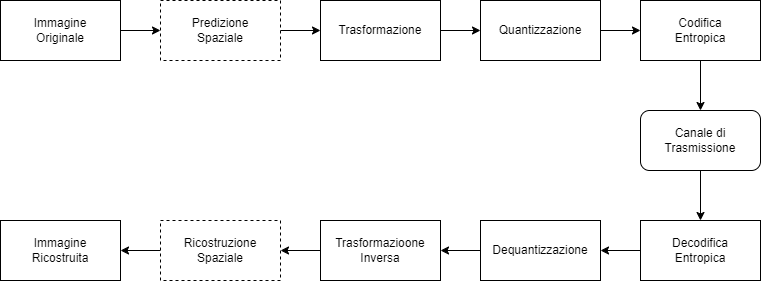
\includegraphics[width=0.8\textwidth]{Immagini/LossyCompressorDiagram.png}
    \caption{Diagramma di compressione Lossy}
    \label{fig:LossyCompressorDiagram}
\end{figure}
 

    \chapter{Metodi tradizionali}
La caratteristica degli algoritmi di compressione tradizionali è quella di usare trasformate statiche all’interno del primo blocco, messe a punto in numerosi anni di ricerca. Questa staticità non permette a questi metodi di adattarsi dinamicamente a tutti i tipi di contenuti delle immagini. Inoltre rende lo sviluppo di un nuovo algoritmo di compressione un processo lungo che richiede anni di studi e progettazione. \cite{cheng2018deep}
Andiamo ora a parlare brevemente dei metodi che andremo a considerare quando valuteremo le prestazioni dei vari algoritmi per poterli confrontare.

\section{Codifica JPEG}
Questo metodo di compressione sviluppato nel 1992, sviluppato dall'omonimo gruppo, è diventato in poco tempo il formato di compressione più diffuso. Nonostante i numerosi tentativi di sostituirlo con formati più moderni questo è rimasto ancora ad oggi il formato più usato, principalmente grazie alla sua facilità implementativa. Il JPEG si basa sull’utilizzo della Discrete Cosine Transform o DCT per realizzare la rappresentazione sparsificata dell’immagine originale. L'immagine viene divisa in blocchi di dimensione $8\:x\:8$ e ad ogni blocco viene applicata la trasformata, i valori prodotti dall'applicazione della trasformata vengono poi quantizzati e codificati con due metodi denominati zig-zag scan e run length coding, al termine viene applicata la codifica entropica. \cite{125072} \\
Possiamo vedere un esempio di compressione con JPEG nella figura \ref{fig:CompressionJPEG}

\section{Codifica JPEG2000}
Nel 2001 con la crescente diffusione di internet, con l’aumento di dimensione e la richiesta di una maggiore qualità delle immagini viene sviluppato, sempre dal Joint Photograph Experts Group (JPEG), questo nuovo formato chiamato appunto JPEG2000 in virtù dell'anno in cui è stato sviluppato.\\
JPEG2000 non utilizza la DCT come il suo predecessore ma viene introdotta una nuova trasformata, la DWT o Discrete Wavelet Transformat, che si propone di meglio identificare e comprimere i bordi delle figure che compongono le immagini, ovvero il dettaglio che ci permette di distinguere le varie regioni all'interno di un’immagine.
Un’ulteriore differenza di JPEG2000 è la sua capacità di comprimere le immagini con qualità progressiva, ovvero permettere di tagliare la stringa di bit in posizioni diverse per ottenere diversi livelli di qualità. Se provassimo a tagliare invece la rappresentazione in bit di JPEG, otterremo un’immagine incompleta.\\
JPEG2000 quindi voleva essere un formato di qualità superiore con una compressione più efficiente.\cite{952804}\\
Possiamo vedere un esempio di compressione con JPEG2000 nella figura \ref{fig:CompressionJPEG2000}

\section{Codifica BPG}
Il formato Better Portable Graphics è stato sviluppato da Fabrice Bellard nel 2014 con l'obbiettivo di sostituire l’ormai affermato formato JPEG. Questo metodo si basa sulla codifica intra-frame del codec HEVC o H.265 \cite{BPGImageformat}.\\
H.265 a differenza di JPEG e JPEG2000 utilizza anche tecniche di predizione spaziale intra-frame per comprimere ulteriormente l’immagine, queste tecniche sfruttano la ridondanza spaziale, come ad esempio le regioni omogenee. Durante la codifica le varie tecniche vengono provate e viene scelta quella migliore. Inoltre la dimensione dei blocchi in cui viene suddivisa l’immagine non è più fissa ma può variare durante la codifica.
La trasformata e la codifica entropica rimangono invece concettualmente simili ai metodi precedenti, ma utilizzano degli algoritmi più avanzati.\\
L’obbiettivo di  Bellard era quello di realizzare un formato molto leggero che potesse fornire immagini più compresse rispetto a JPEG, ma con una qualità superiore, di cui possiamo vedere un esempio nella figura \ref{fig:CompressionBPG}

\section{Codifica VVC}
Versatile Video Coding (VVC) o H.266 è lo standard di codifica video più recente, finalizzato nel luglio 2020. È stato sviluppato dal Joint Video Experts Team (JVET) dell'ITU-T Video Coding Experts Group (VCEG) e dell'ISO/IEC Moving Picture Experts Group (MPEG) per soddisfare la crescente richiesta di una migliore compressione video, per supportare una più ampia gamma di contenuti multimediali attuali e applicazioni emergenti come contenuti in High Dynamic Range (HDR), a 360°, per la Realtà Virtuale (VR) o la Realtà Aumentata (AR) \cite{9503377}.\\
Sebbene sia stato sviluppato per la compressione video, fornisce ottimi risultati anche per la compressione di immagini con metodo intra.\\
Come il suo predecessore, H.266 utilizza tecniche di predizione spaziale intra-frame e blocchi a dimensione variabile. A differenza del suo predecessore però le tecniche di predizione sono molte di più e più elaborate, e la dimensione di blocco può variare con più libertà.
La trasformata e la codifica entropica rimangono simili ai metodi precedenti, ma utilizzano degli algoritmi più avanzati.\\
L’algoritmo di codifica VVC rappresenta l’attuale stato dell’arte per la compressione di video ed immagini, ne possiamo vedere un esempio nella figura \ref{fig:CompressionVVC}\\
\newpage

\begin{figure}[h!]
    \centering
    \begin{subfigure}[]{0.3\textwidth}
        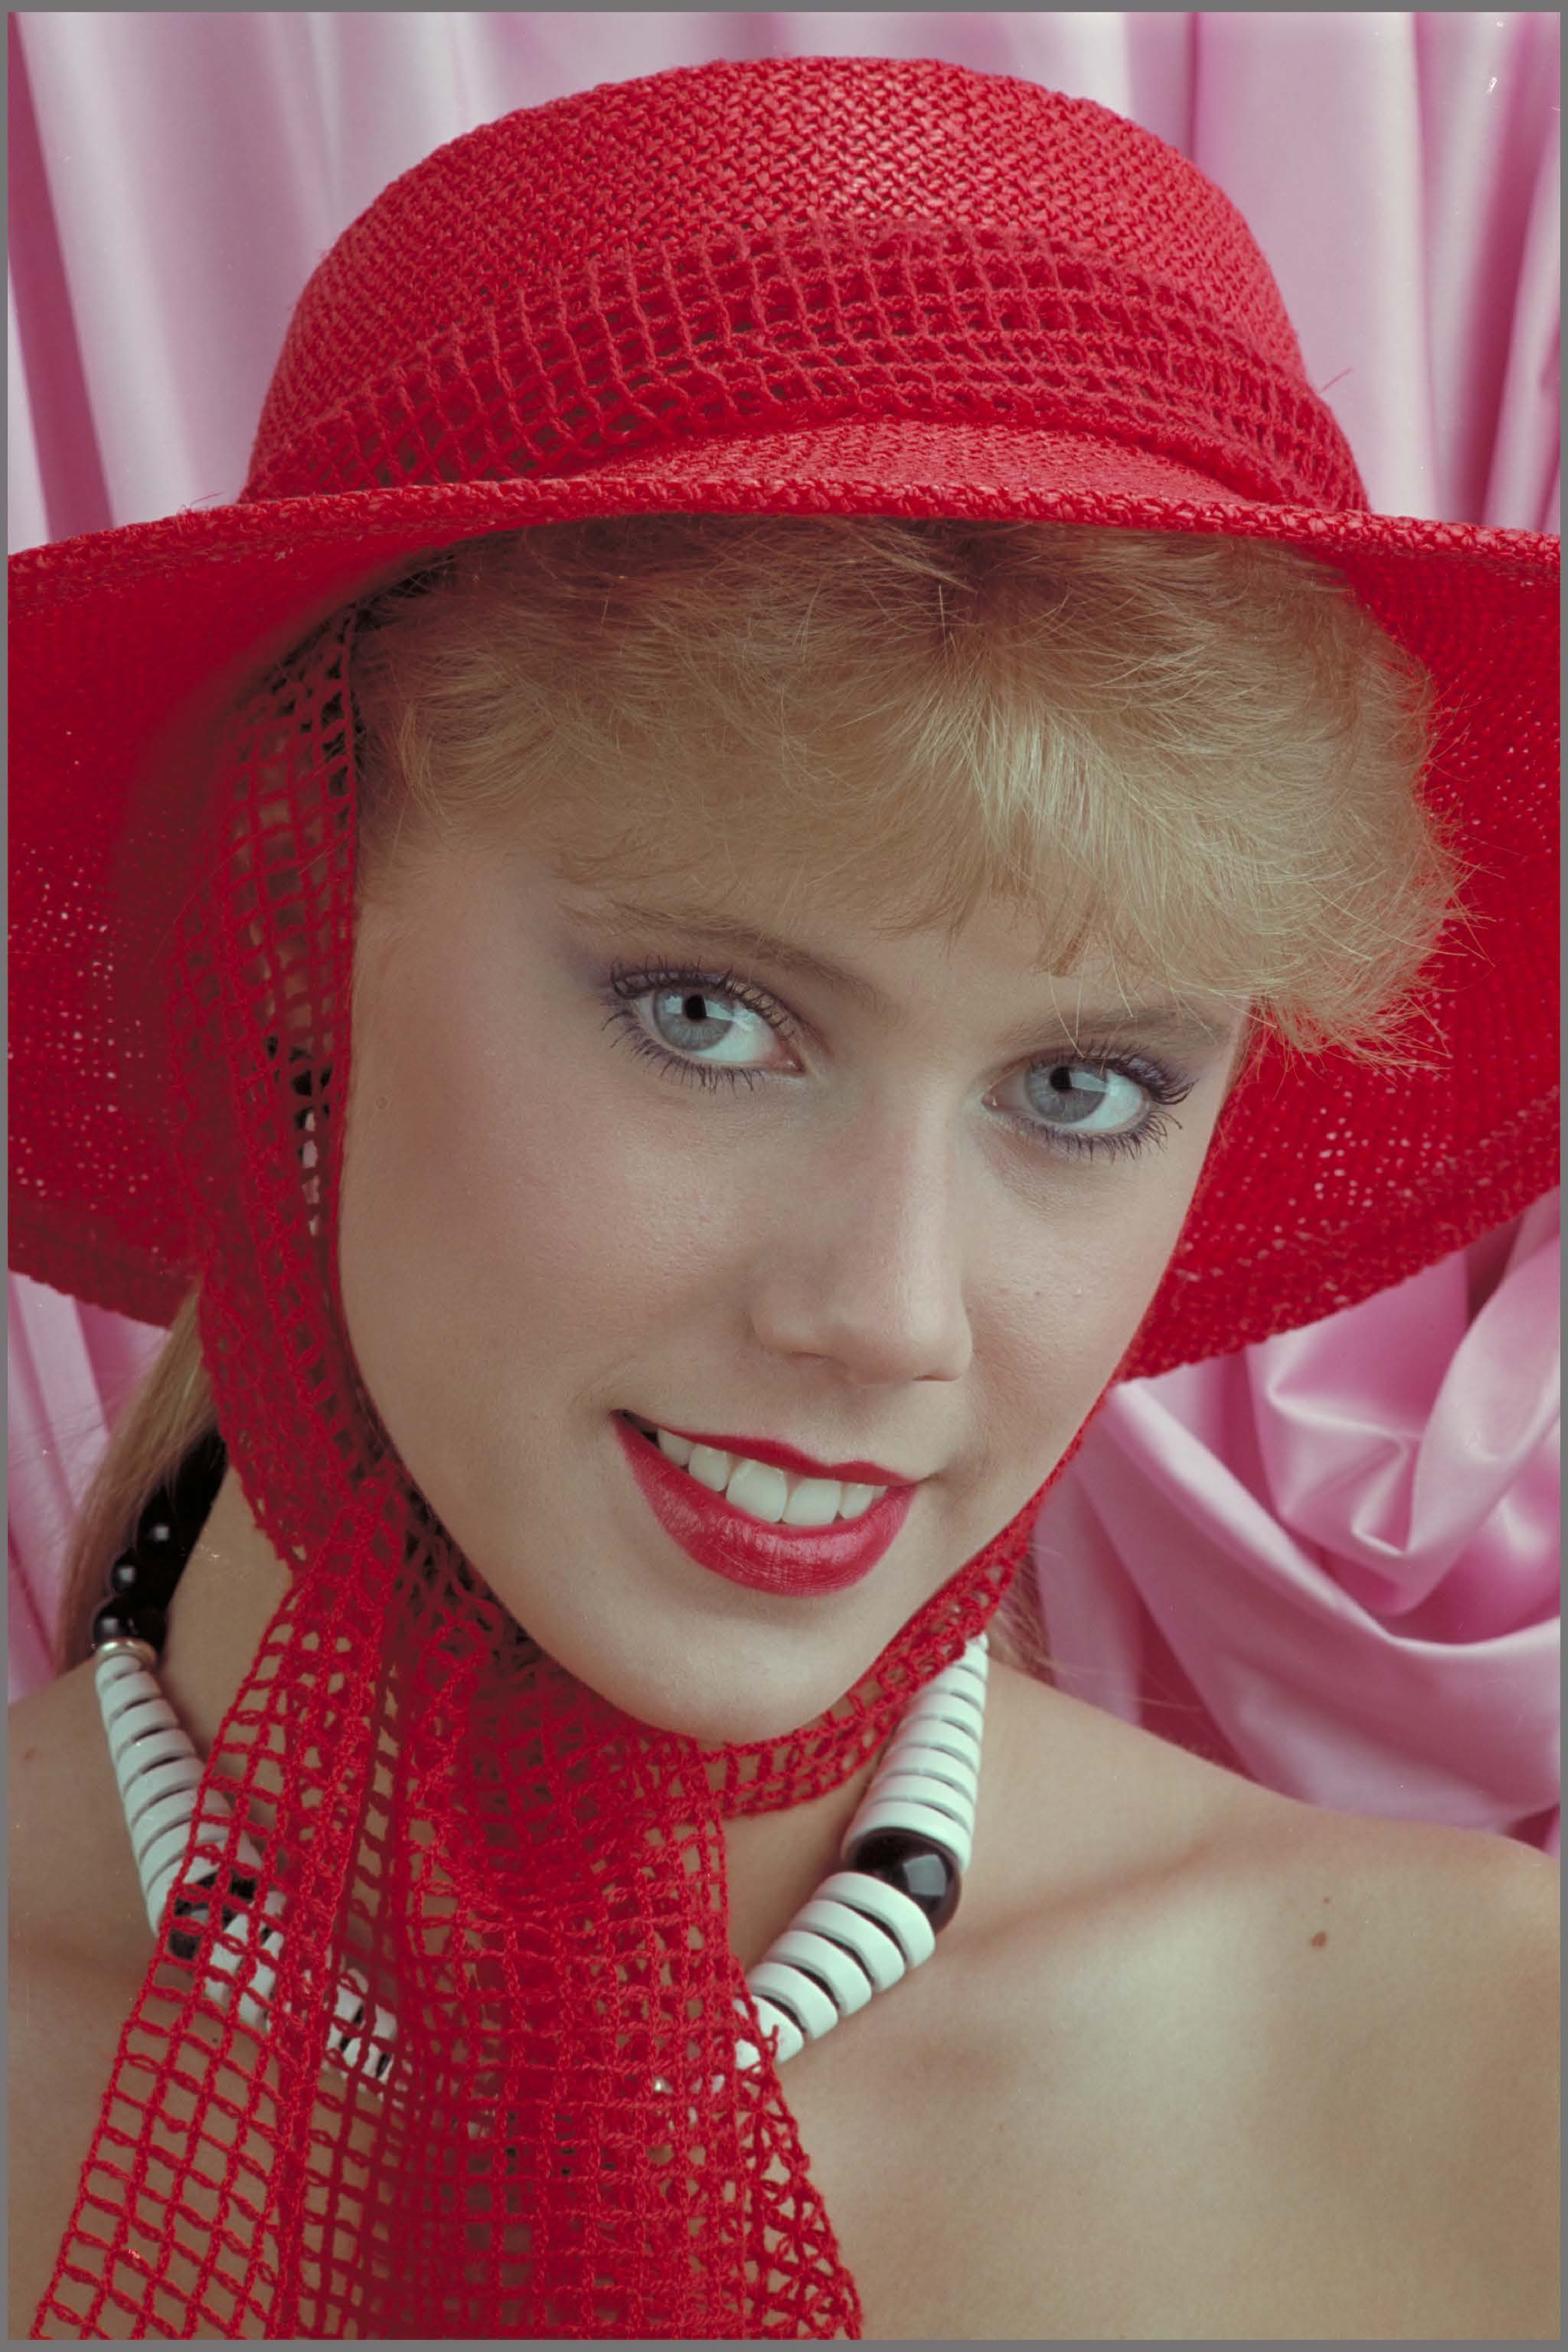
\includegraphics[width=\textwidth]{Immagini/IMAGES/PNG_IMG0004.pdf}
        \caption{Originale}
        \label{fig:OriginalJPEG}
    \end{subfigure}
    \hspace*{1.5cm}
    \begin{subfigure}[]{0.3\textwidth}
        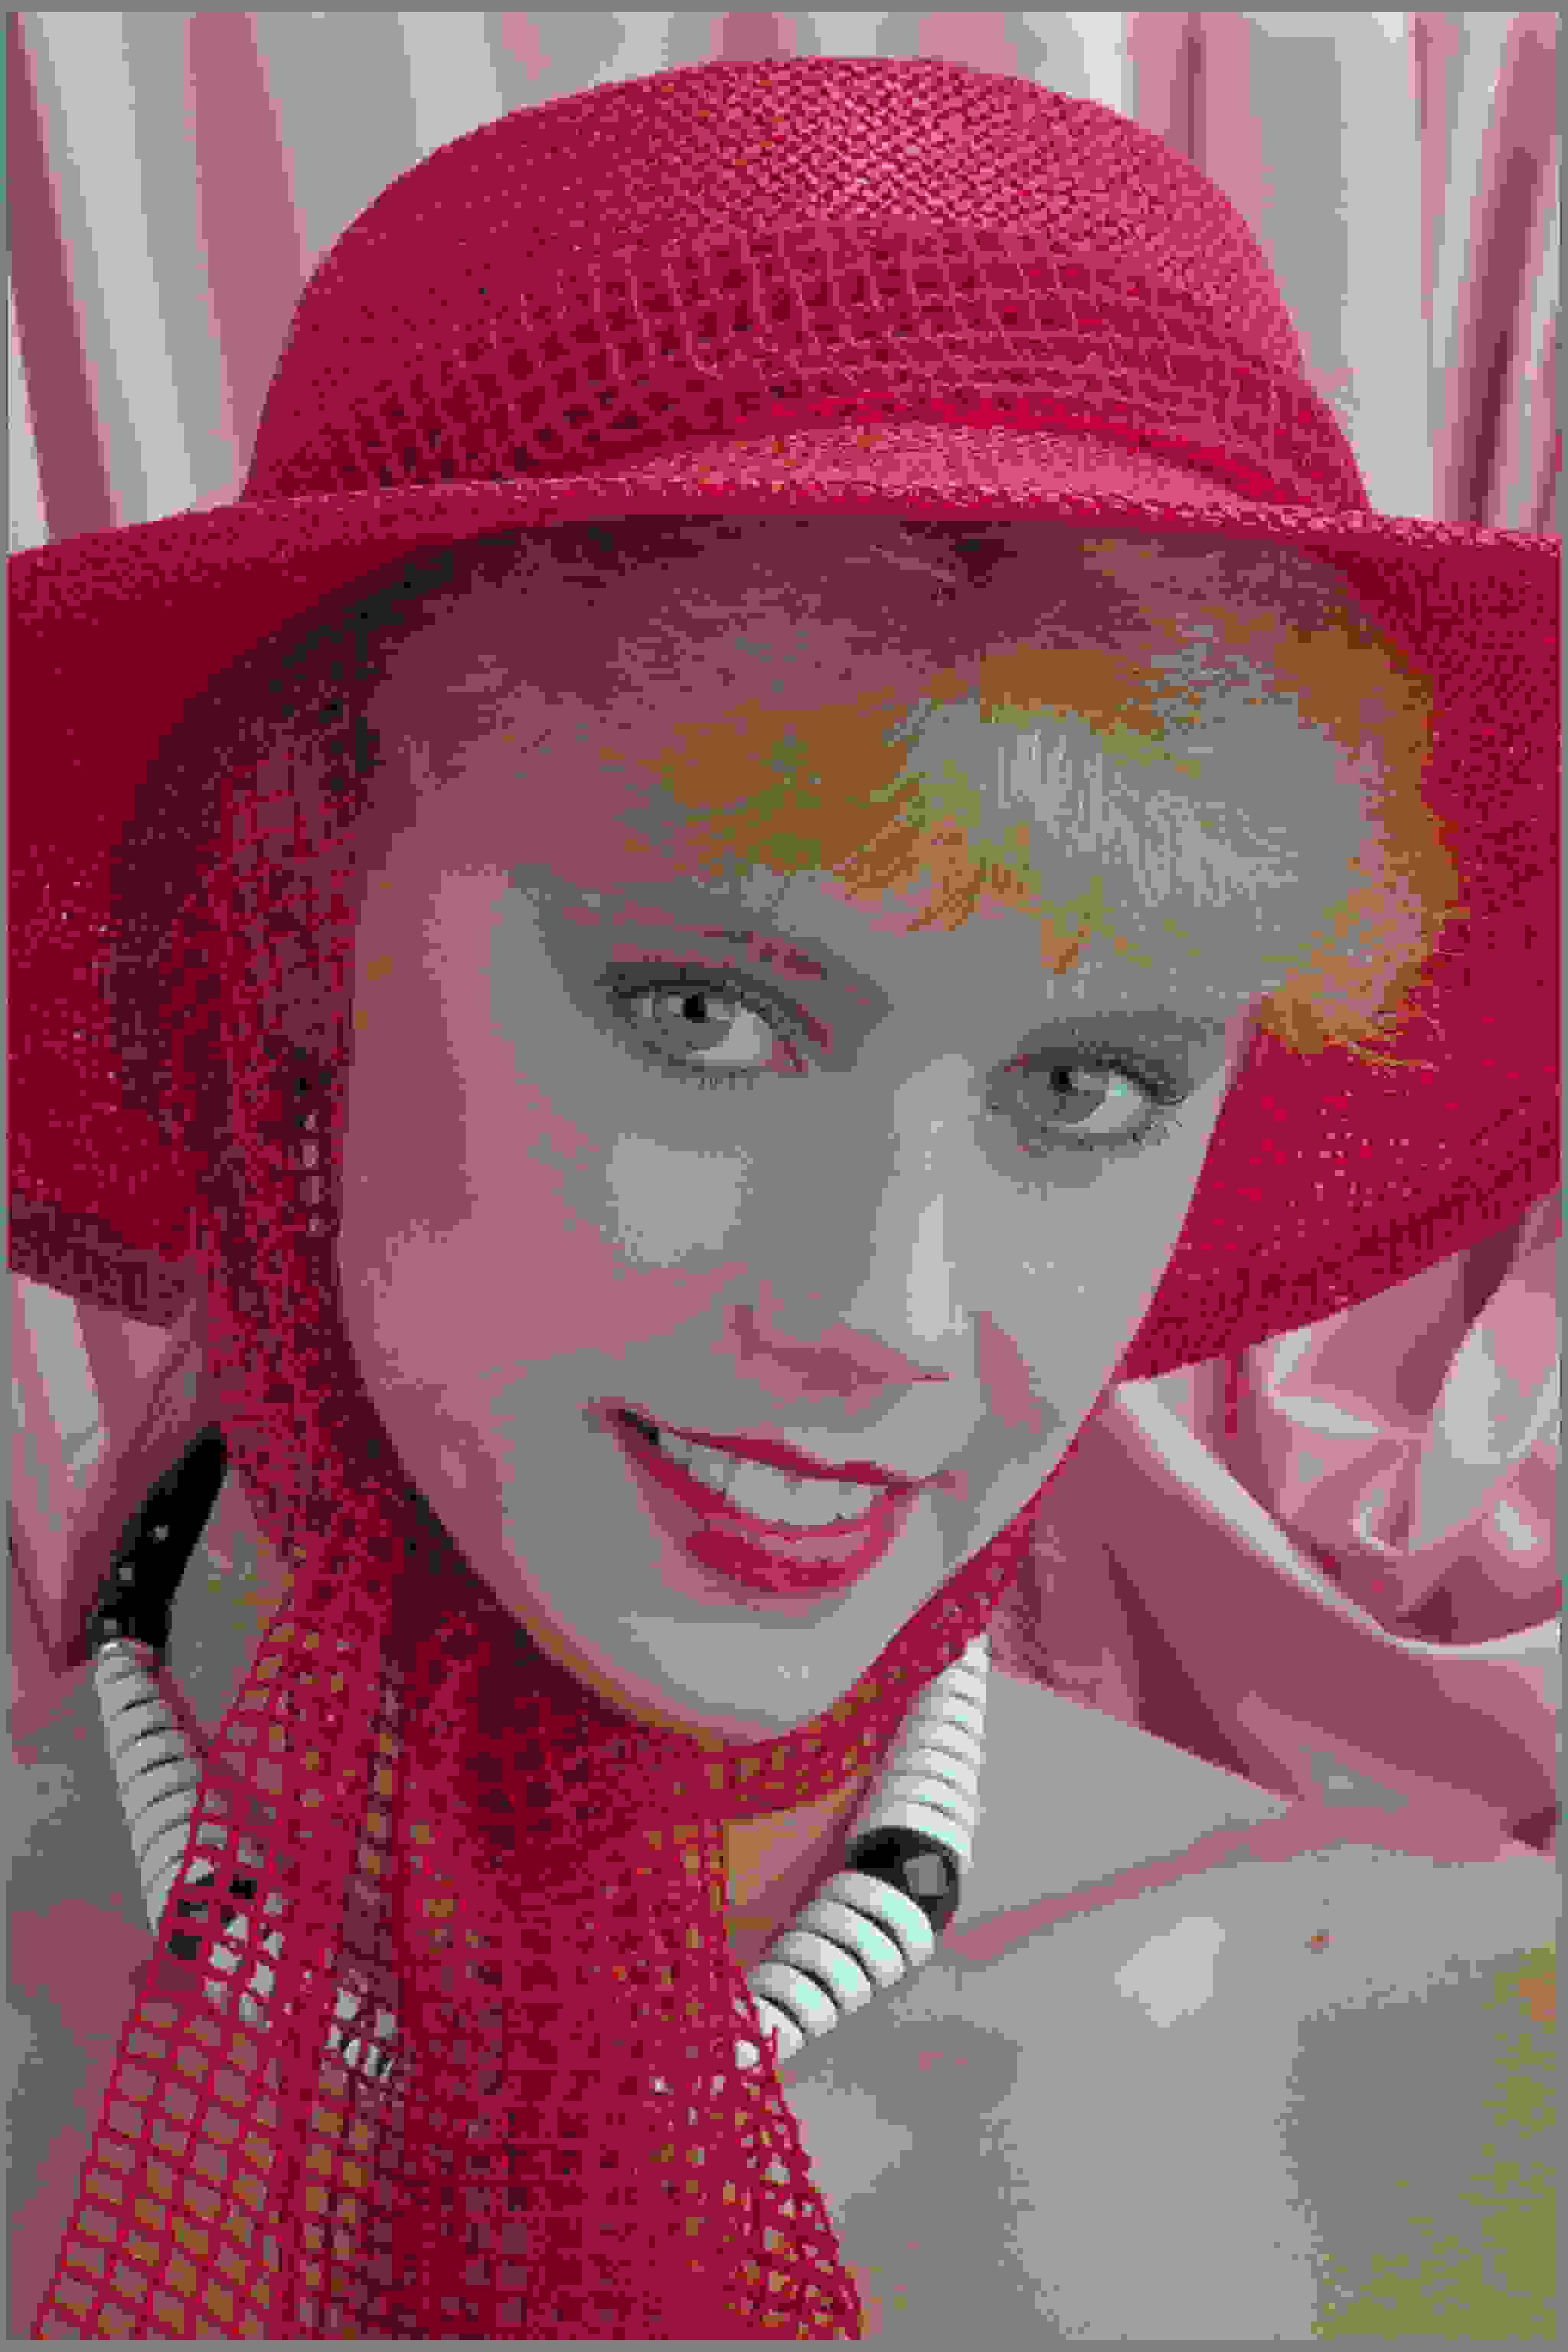
\includegraphics[width=\textwidth]{Immagini/IMAGES/JPEG_1_IMG0004.pdf}
        \caption{JPEG}
        \label{fig:CompressedJPEG}
    \end{subfigure}
    \caption{Confronto PNG con JPEG a 0.167 bpp}
    \label{fig:CompressionJPEG}
\end{figure}

\begin{figure}[h!]
    \centering
    \begin{subfigure}[]{0.3\textwidth}
        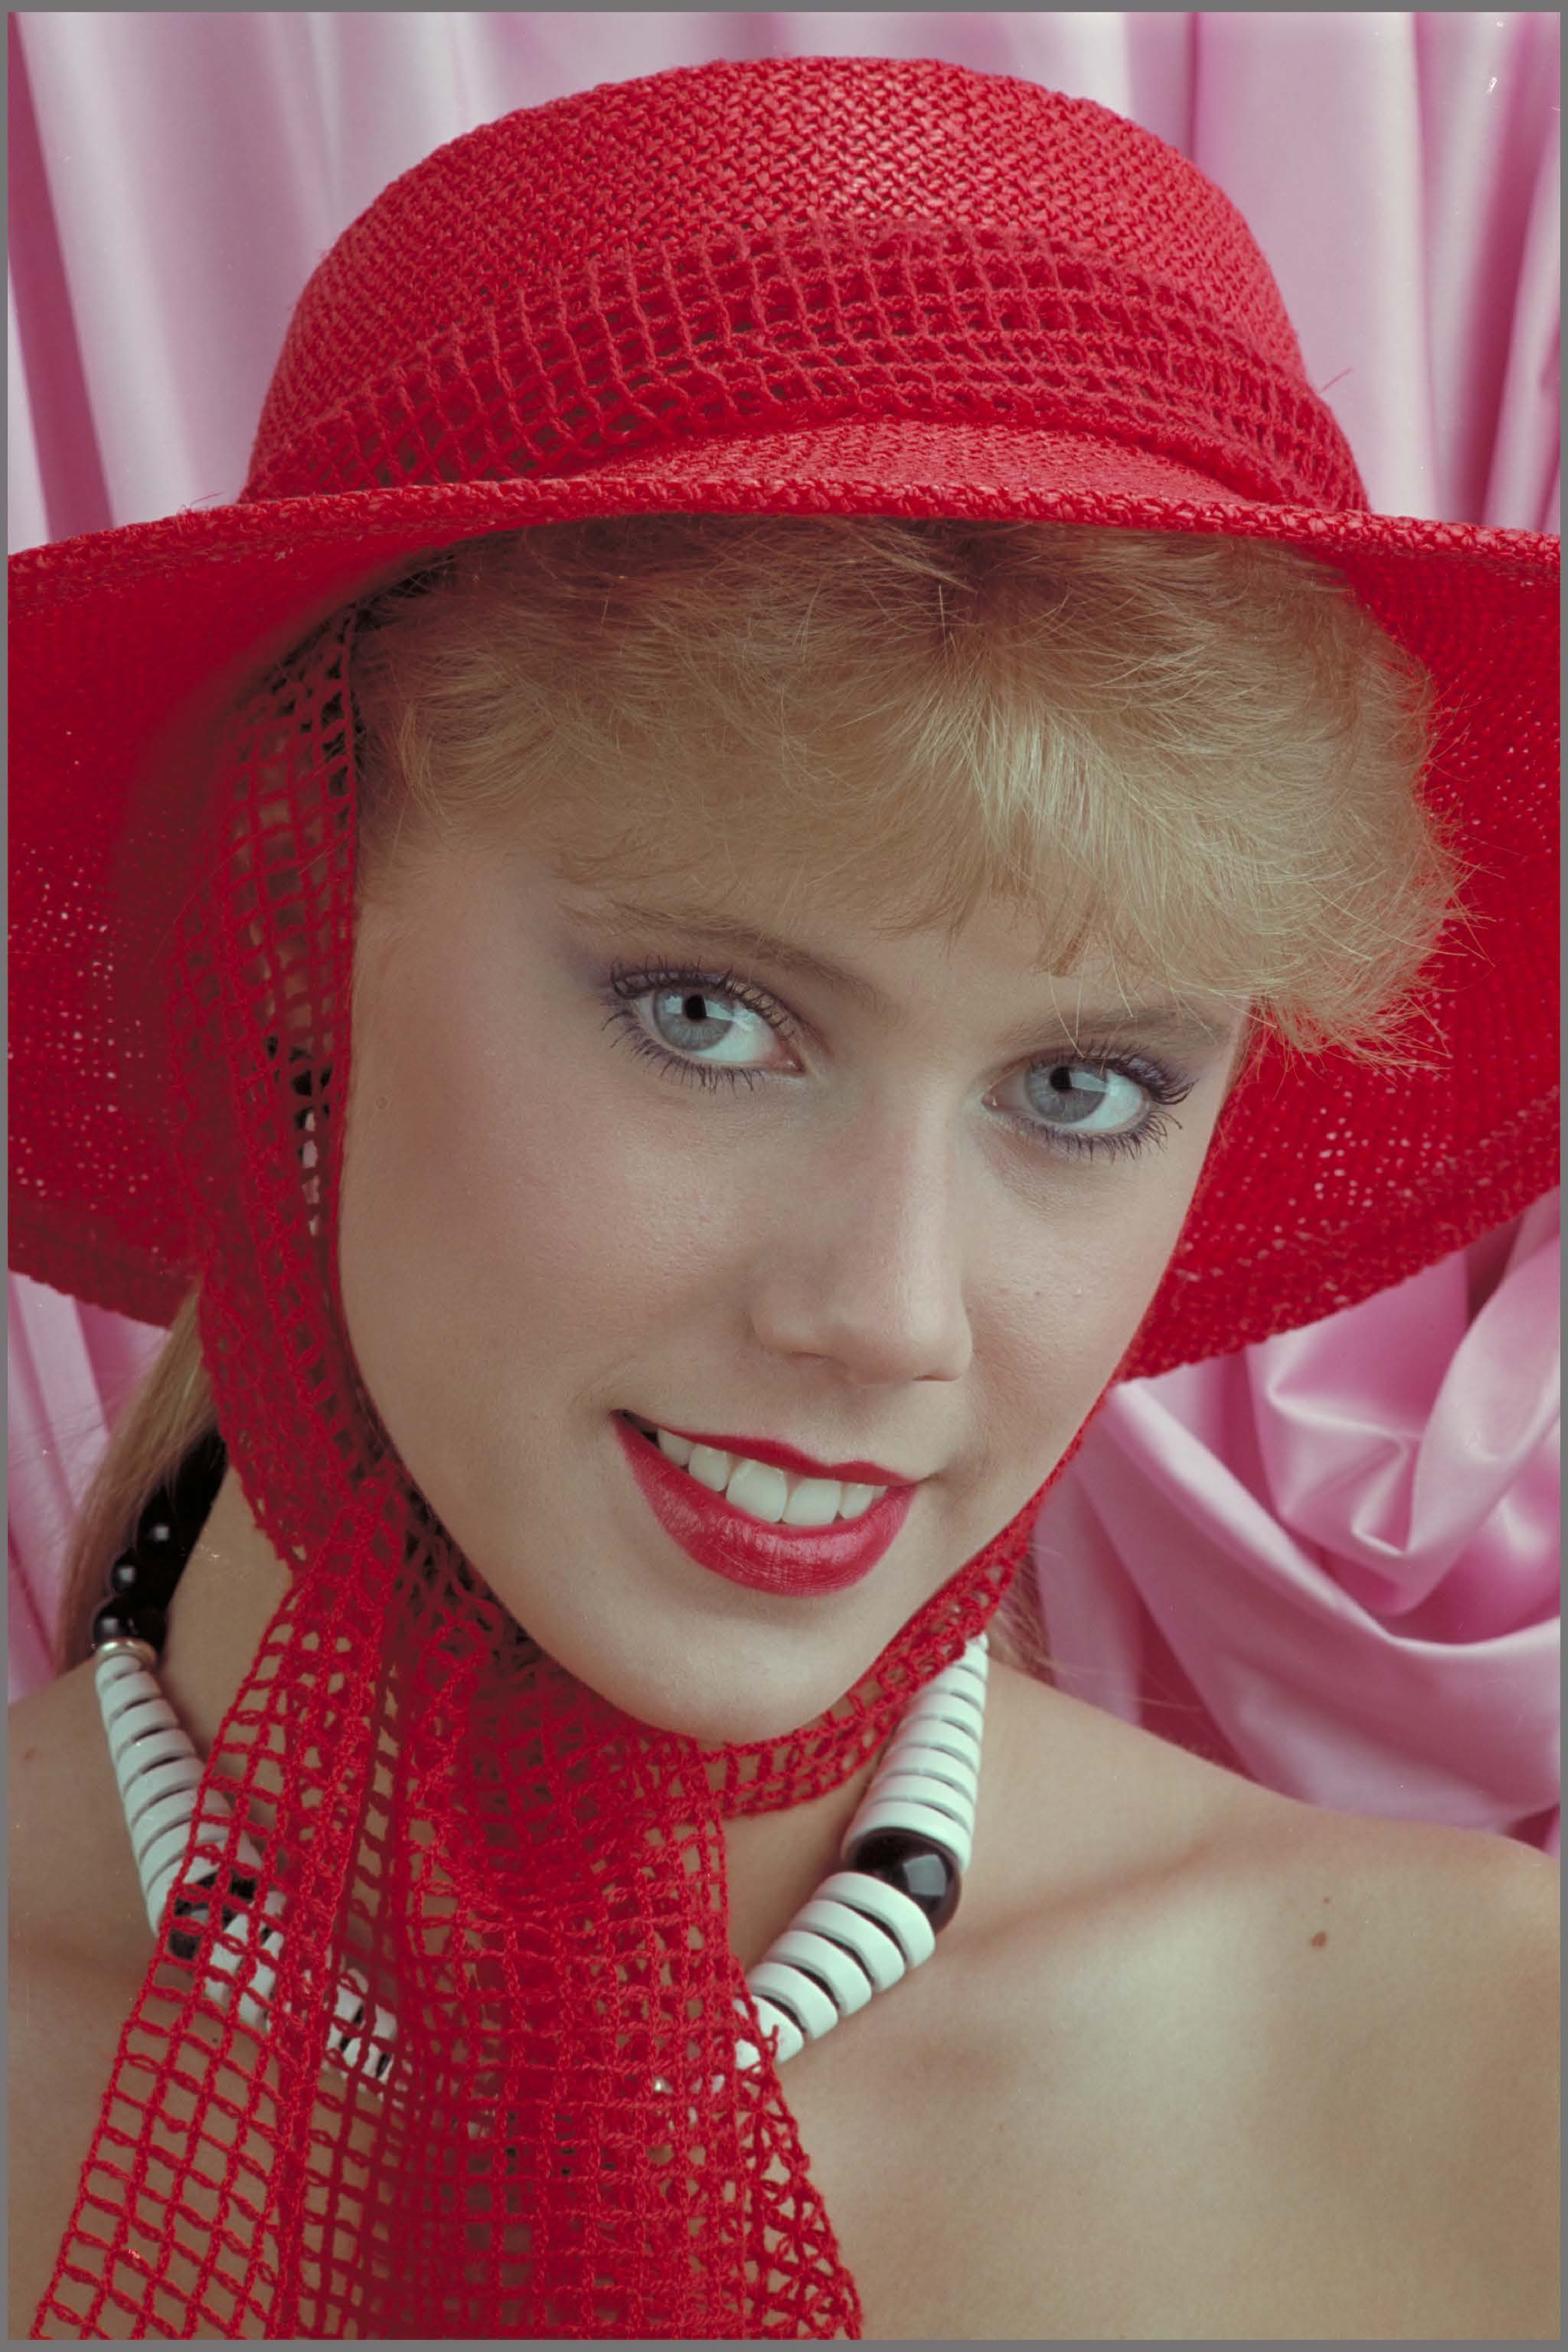
\includegraphics[width=\textwidth]{Immagini/IMAGES/PNG_IMG0004.pdf}
        \caption{Originale}
        \label{fig:OriginalJPEG2000}
    \end{subfigure}
    \hspace*{1.5cm}
    \begin{subfigure}[]{0.3\textwidth}
        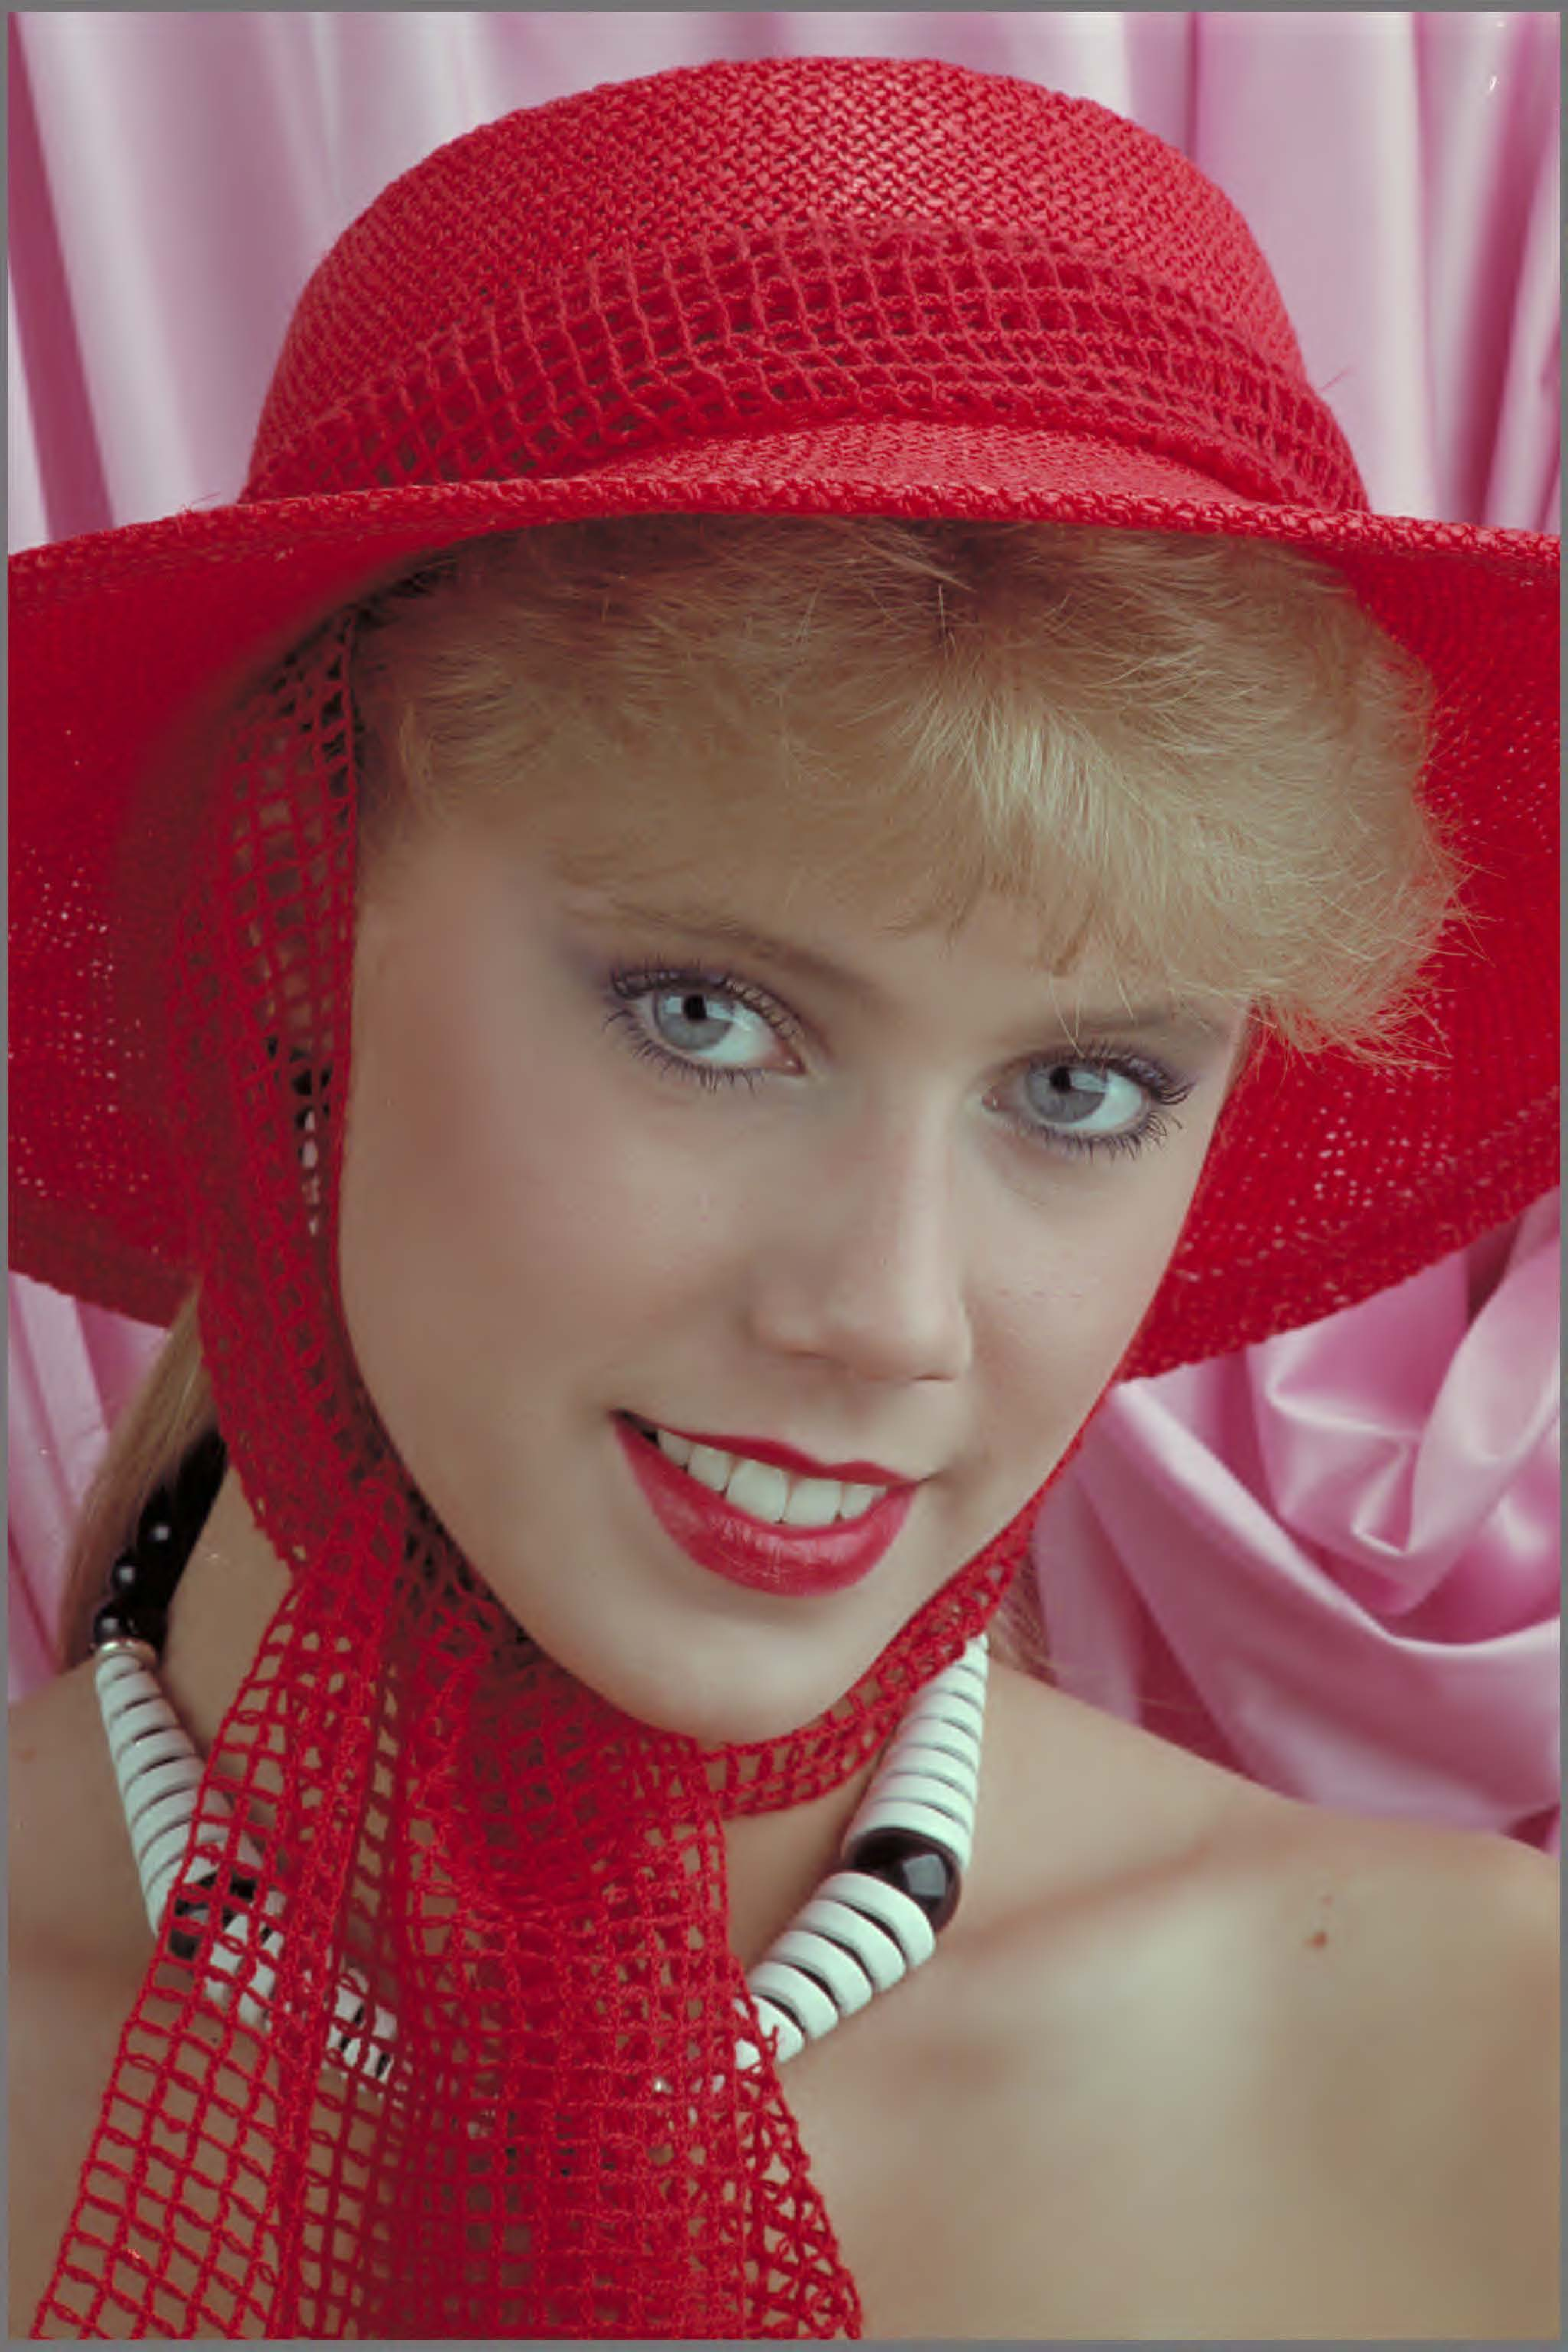
\includegraphics[width=\textwidth]{Immagini/IMAGES/JPEG2000_2_IMG0004.pdf}
        \caption{JPEG2000}
        \label{fig:CompressedJPEG2000}
    \end{subfigure}
    \caption{Confronto PNG con JPEG2000 a 0.171 bpp}
    \label{fig:CompressionJPEG2000}
\end{figure}

\newpage
\begin{figure}[h!]
    \centering
    \begin{subfigure}[]{0.3\textwidth}
        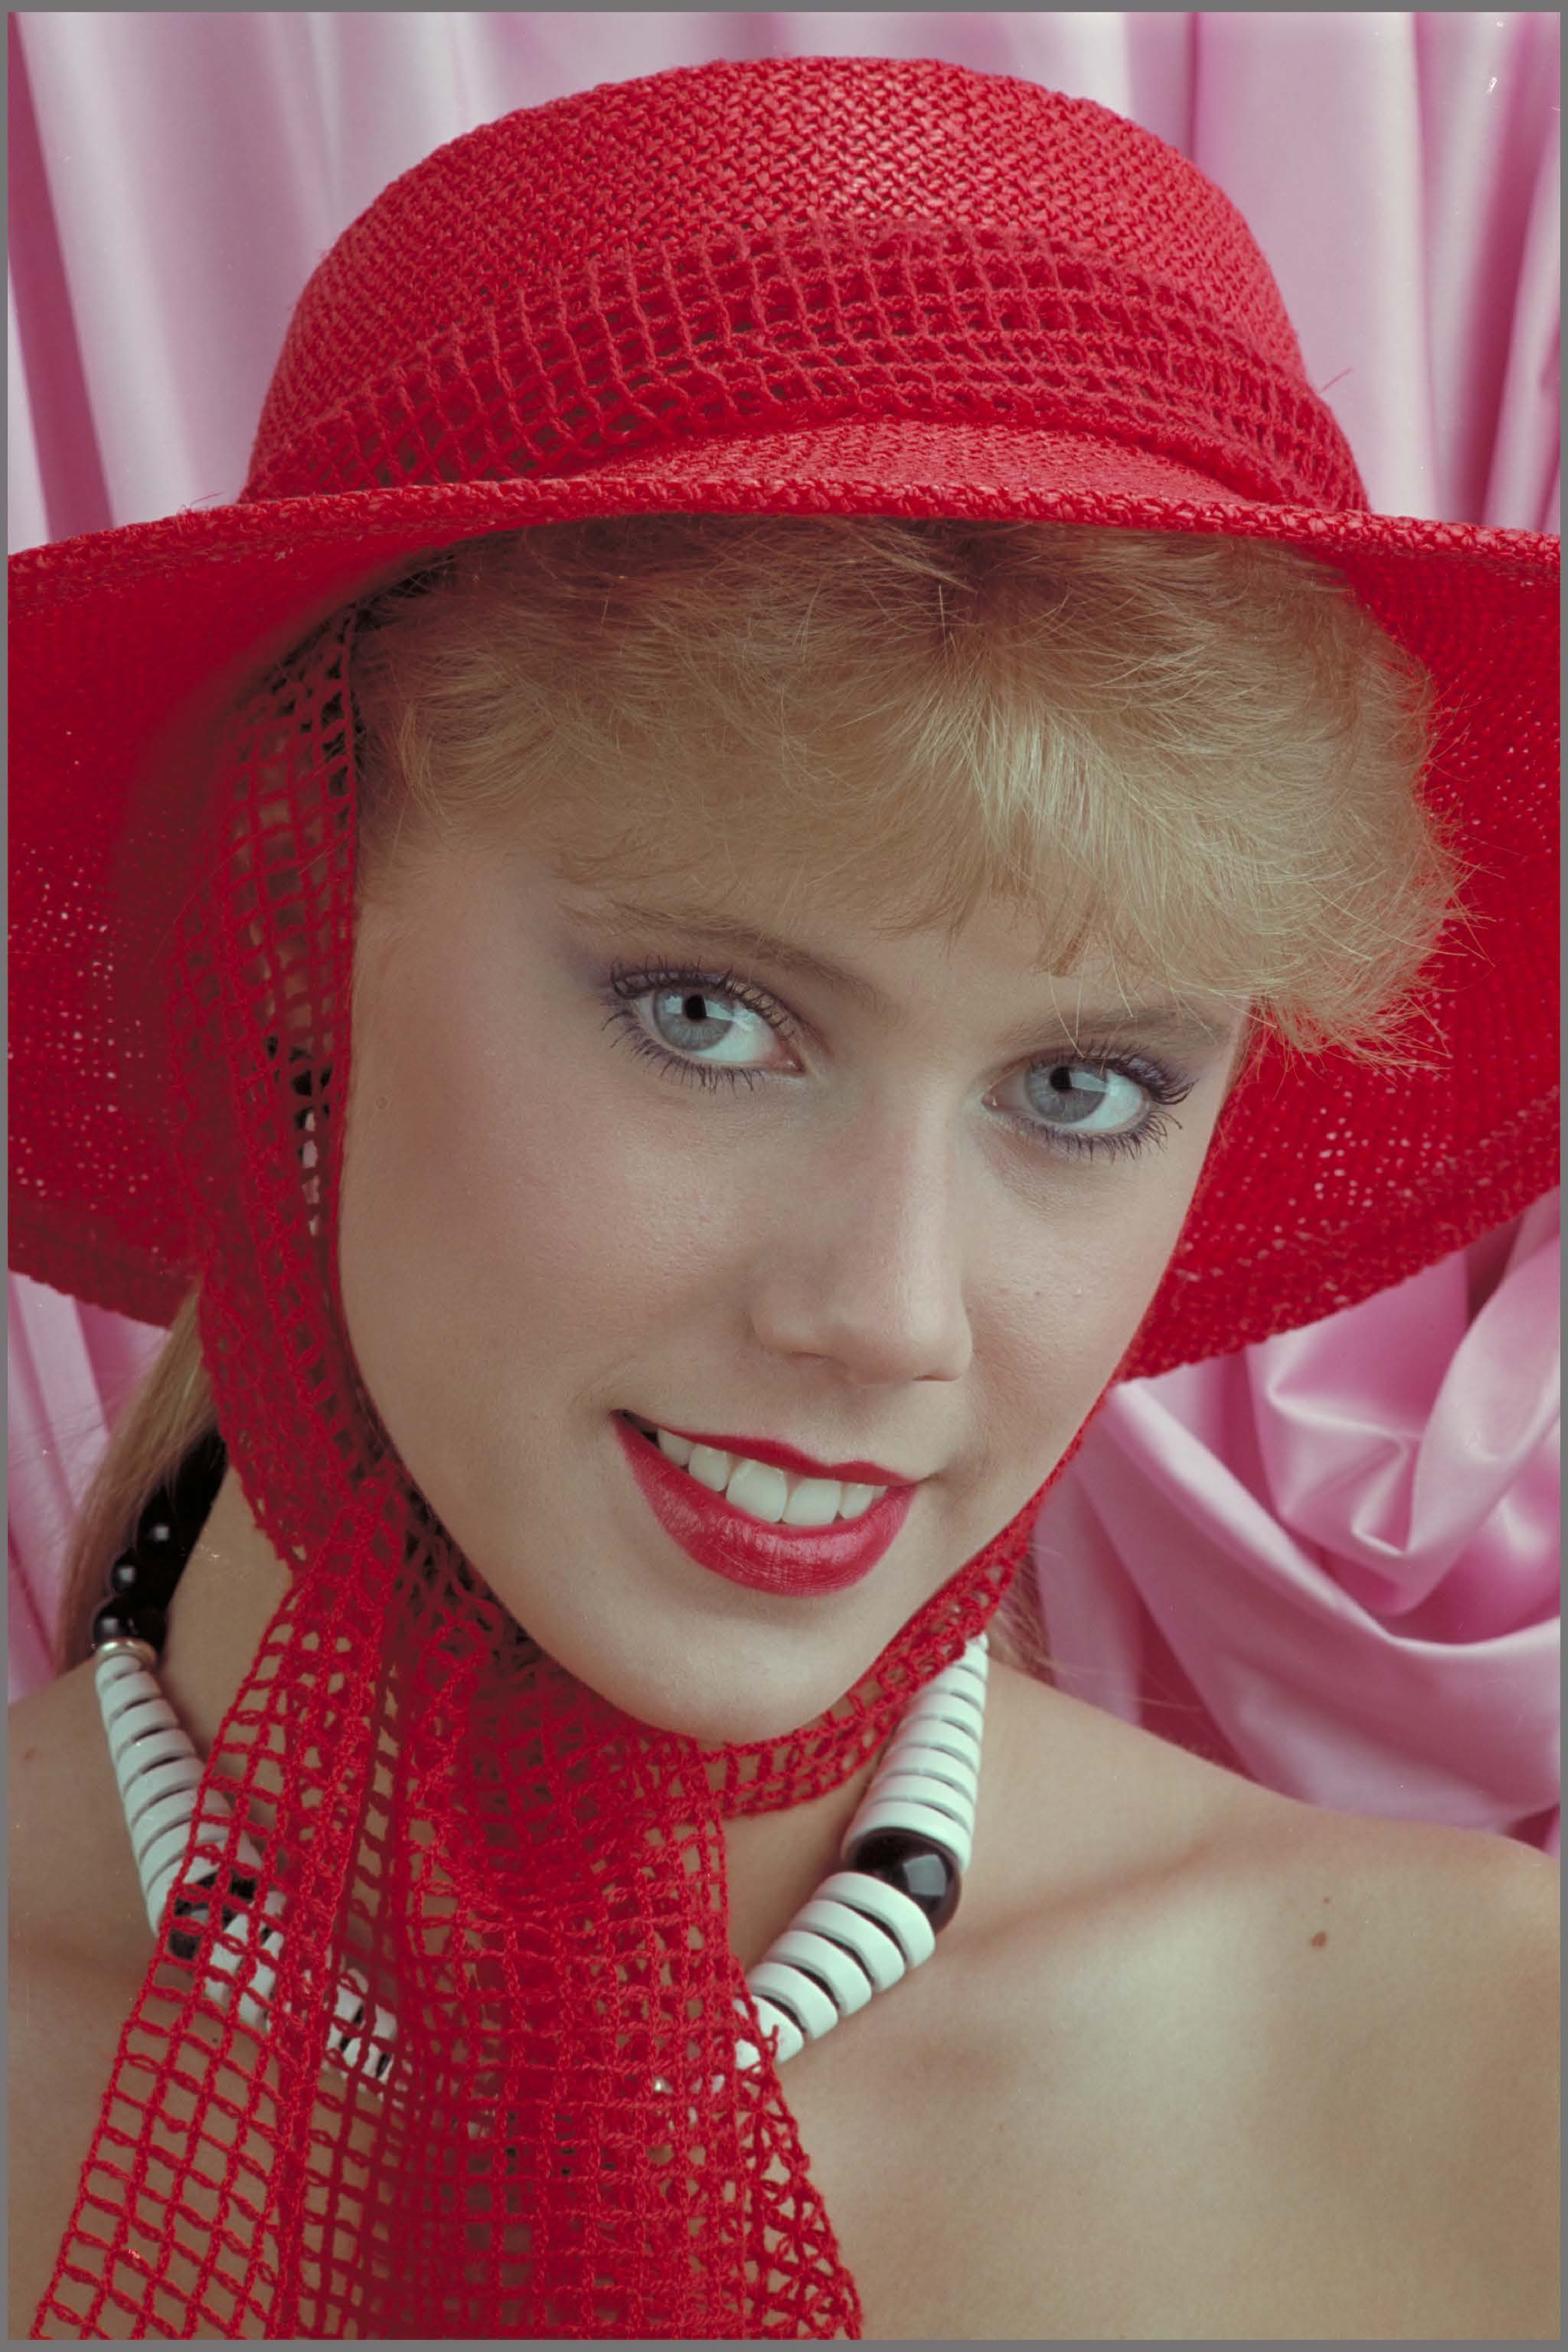
\includegraphics[width=\textwidth]{Immagini/IMAGES/PNG_IMG0004.pdf}
        \caption{Originale}
        \label{fig:OriginalBPG}
    \end{subfigure}
    \hspace*{1.5cm}
    \begin{subfigure}[]{0.3\textwidth}
        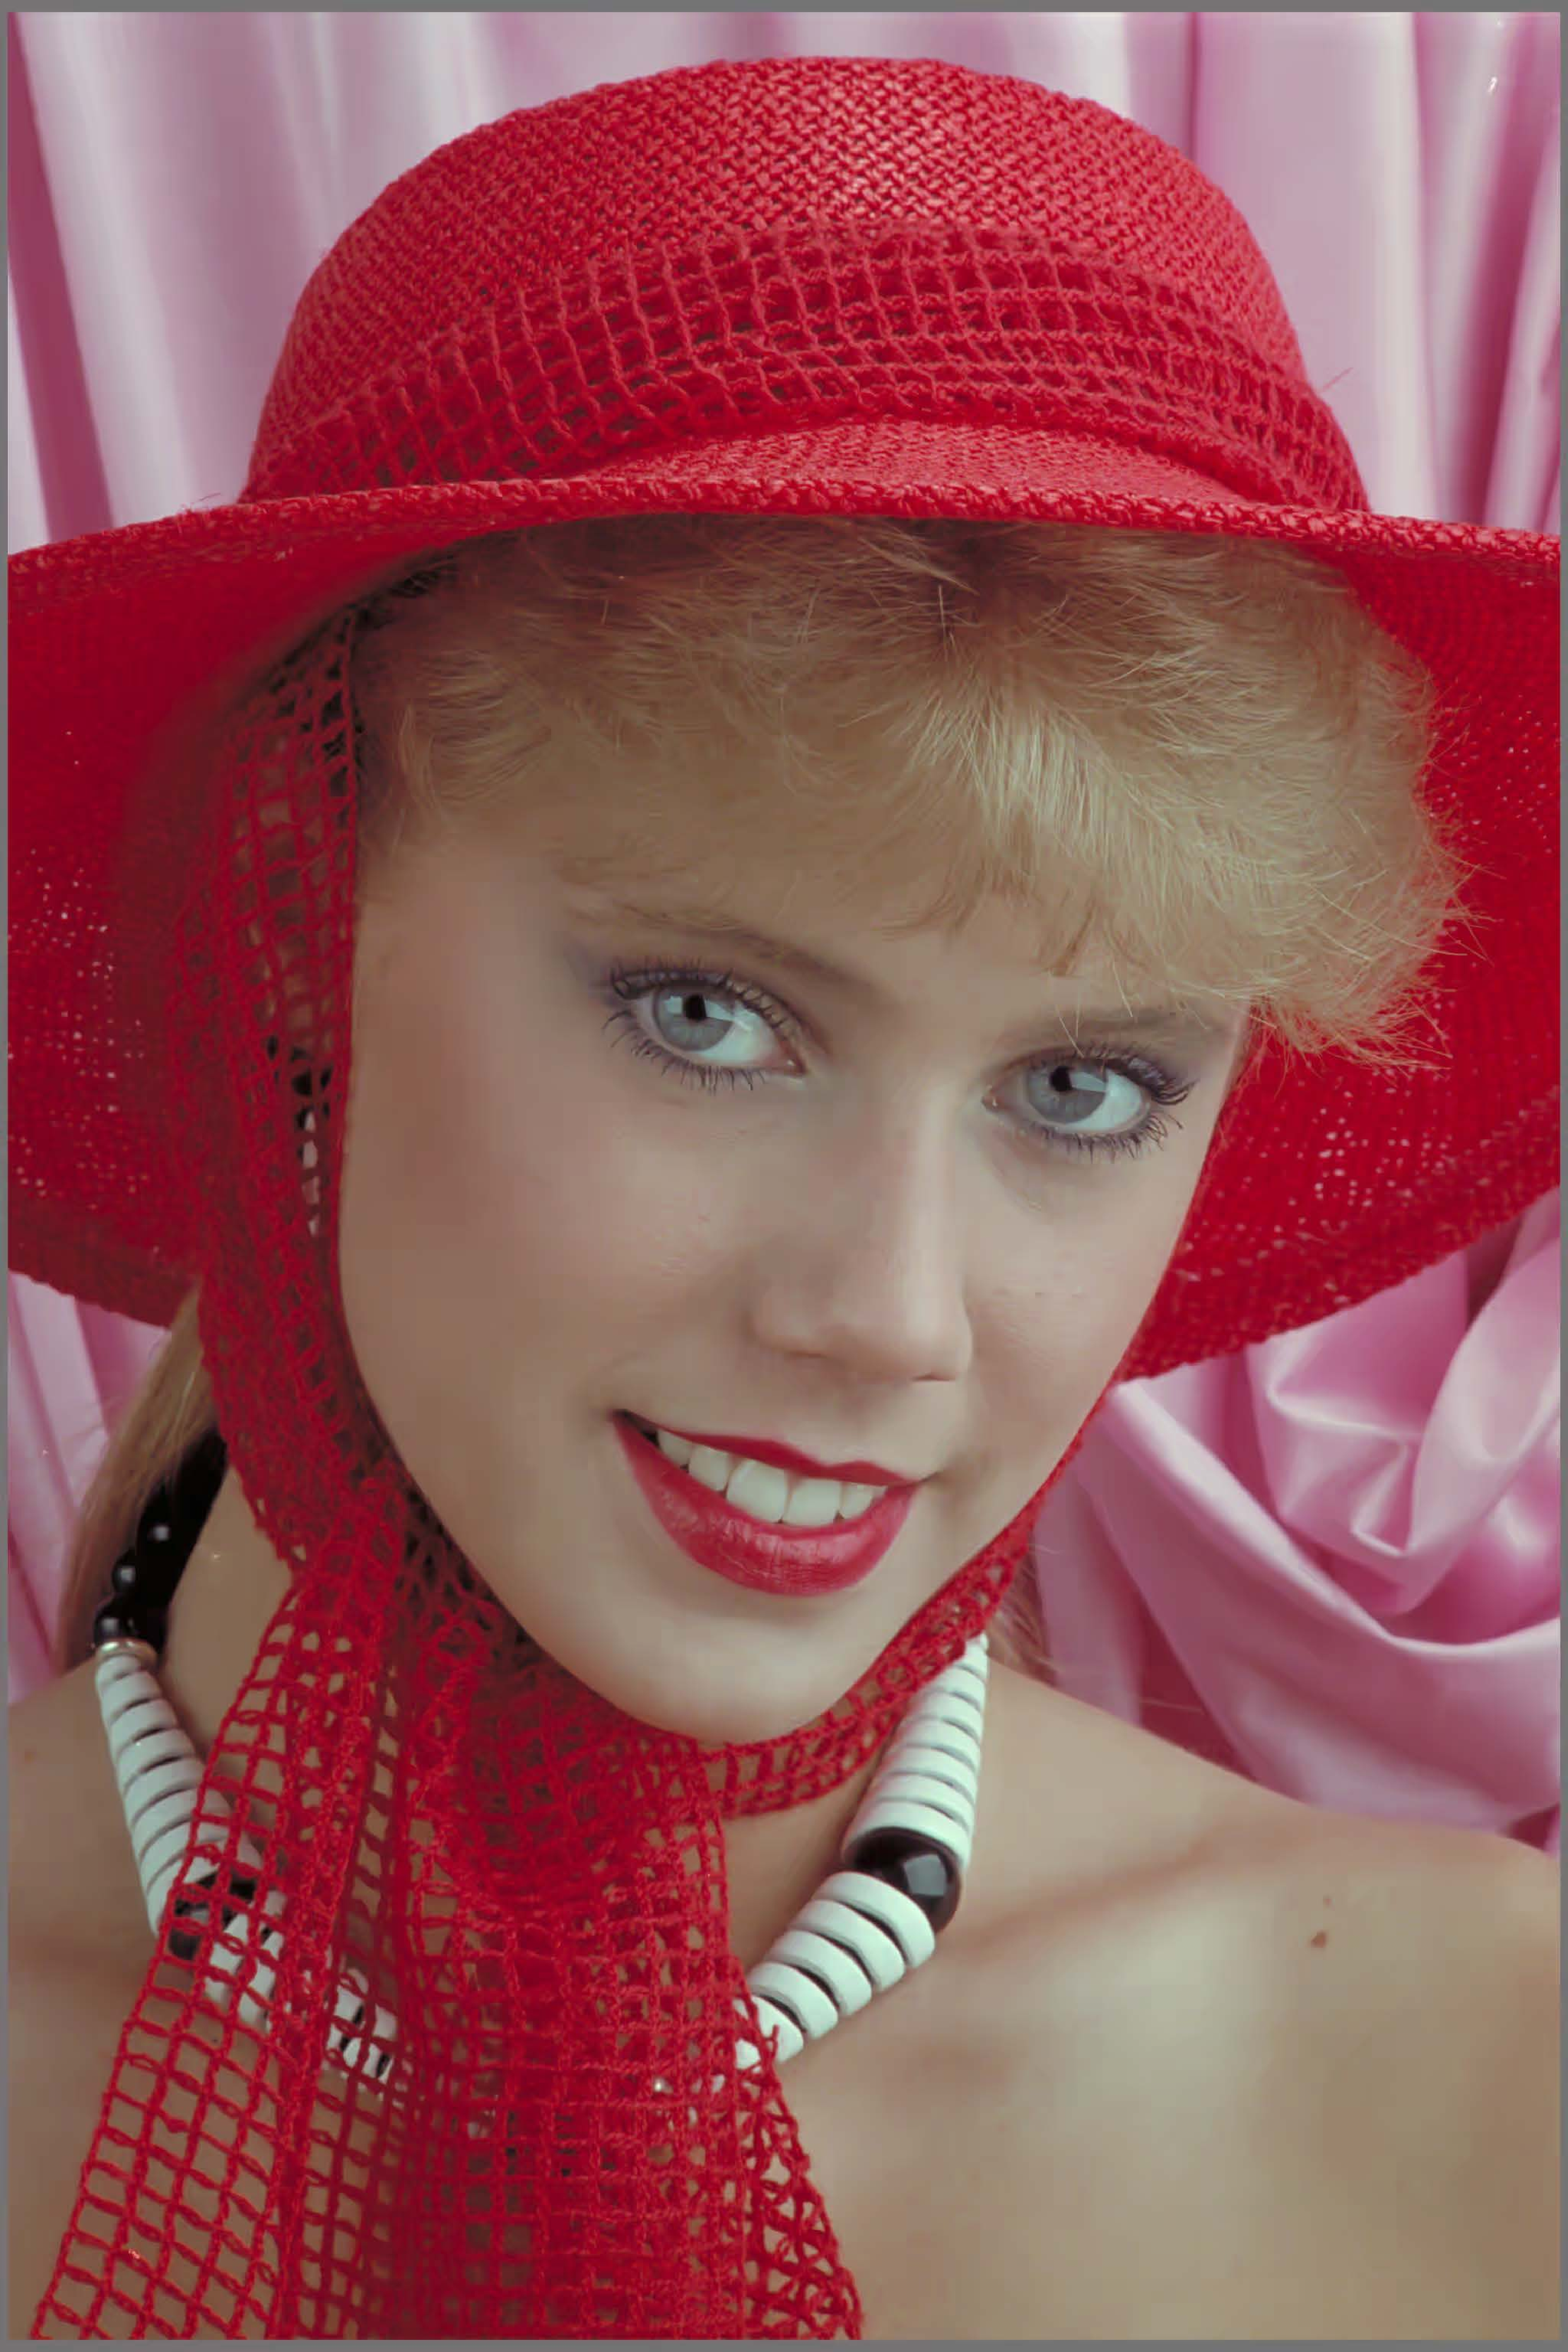
\includegraphics[width=\textwidth]{Immagini/IMAGES/BPG_3_IMG0004.pdf}
        \caption{BPG}
        \label{fig:CompressedBPG}
    \end{subfigure}
    \caption{Confronto PNG con BPG a 0.156 bpp}
    \label{fig:CompressionBPG}
\end{figure}

\begin{figure}[h!]
    \centering
    \begin{subfigure}[]{0.3\textwidth}
        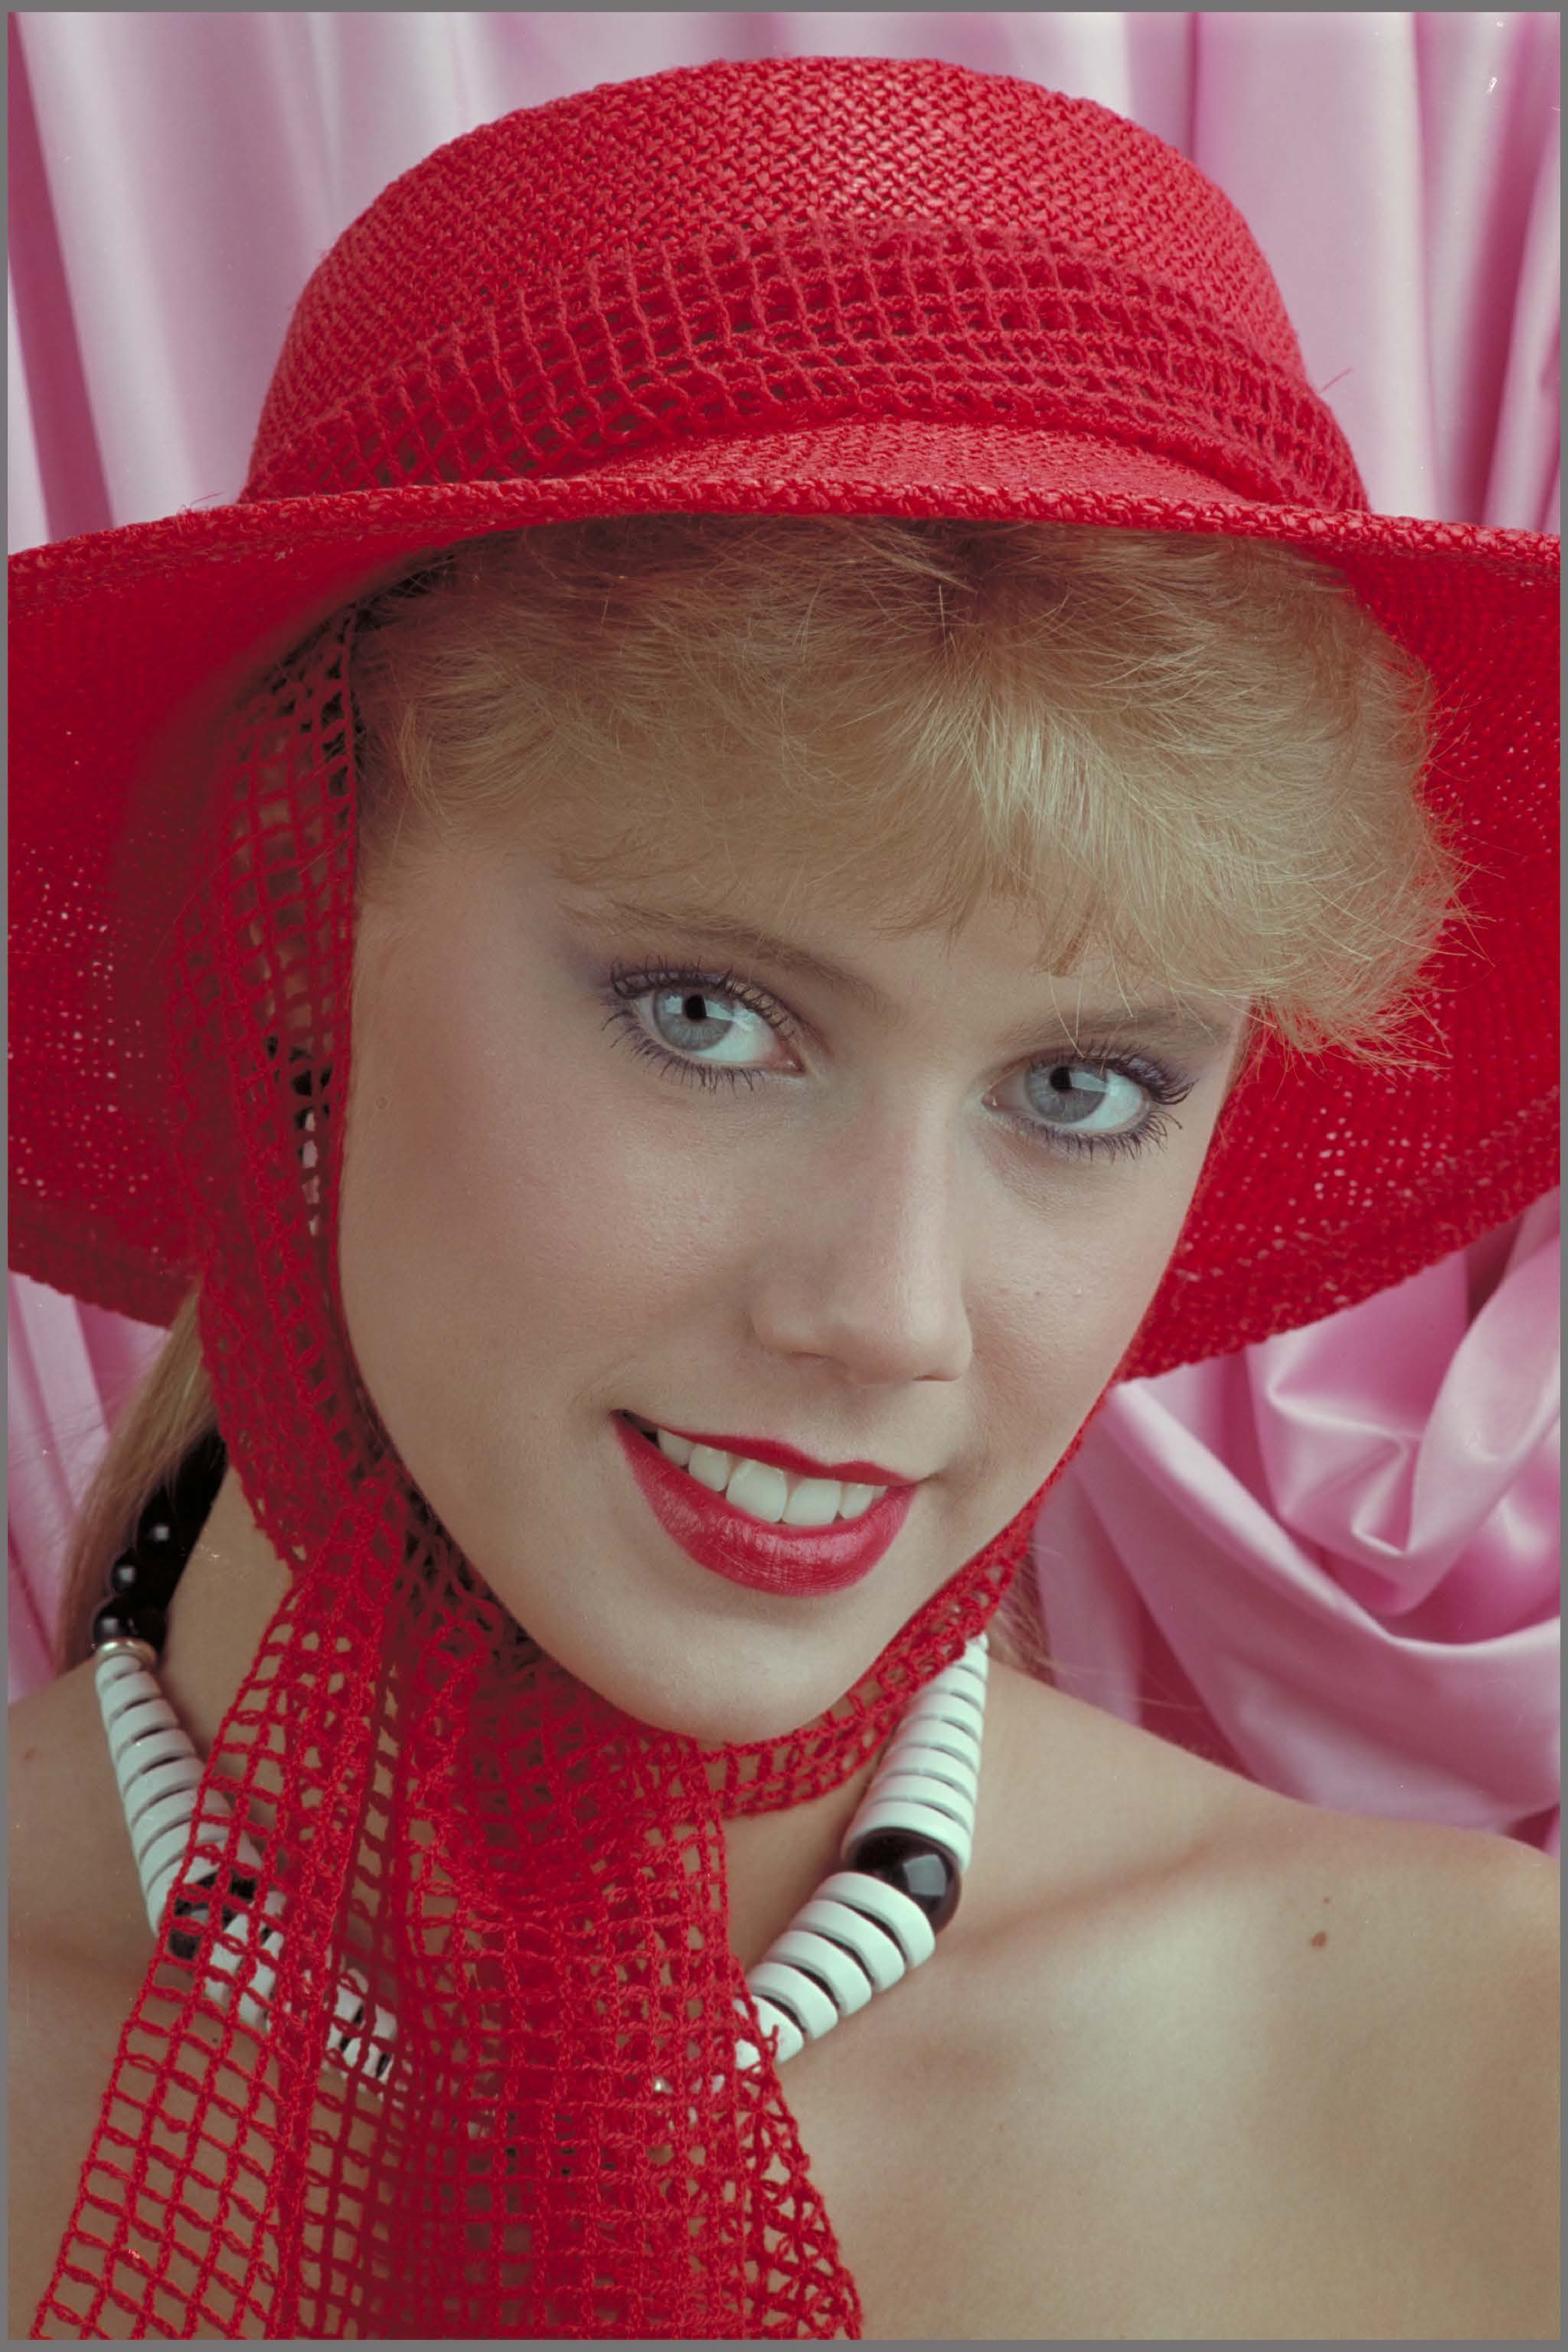
\includegraphics[width=\textwidth]{Immagini/IMAGES/PNG_IMG0004.pdf}
        \caption{Originale}
        \label{fig:OriginalVVC}
    \end{subfigure}
    \hspace*{1.5cm}
    \begin{subfigure}[]{0.3\textwidth}
        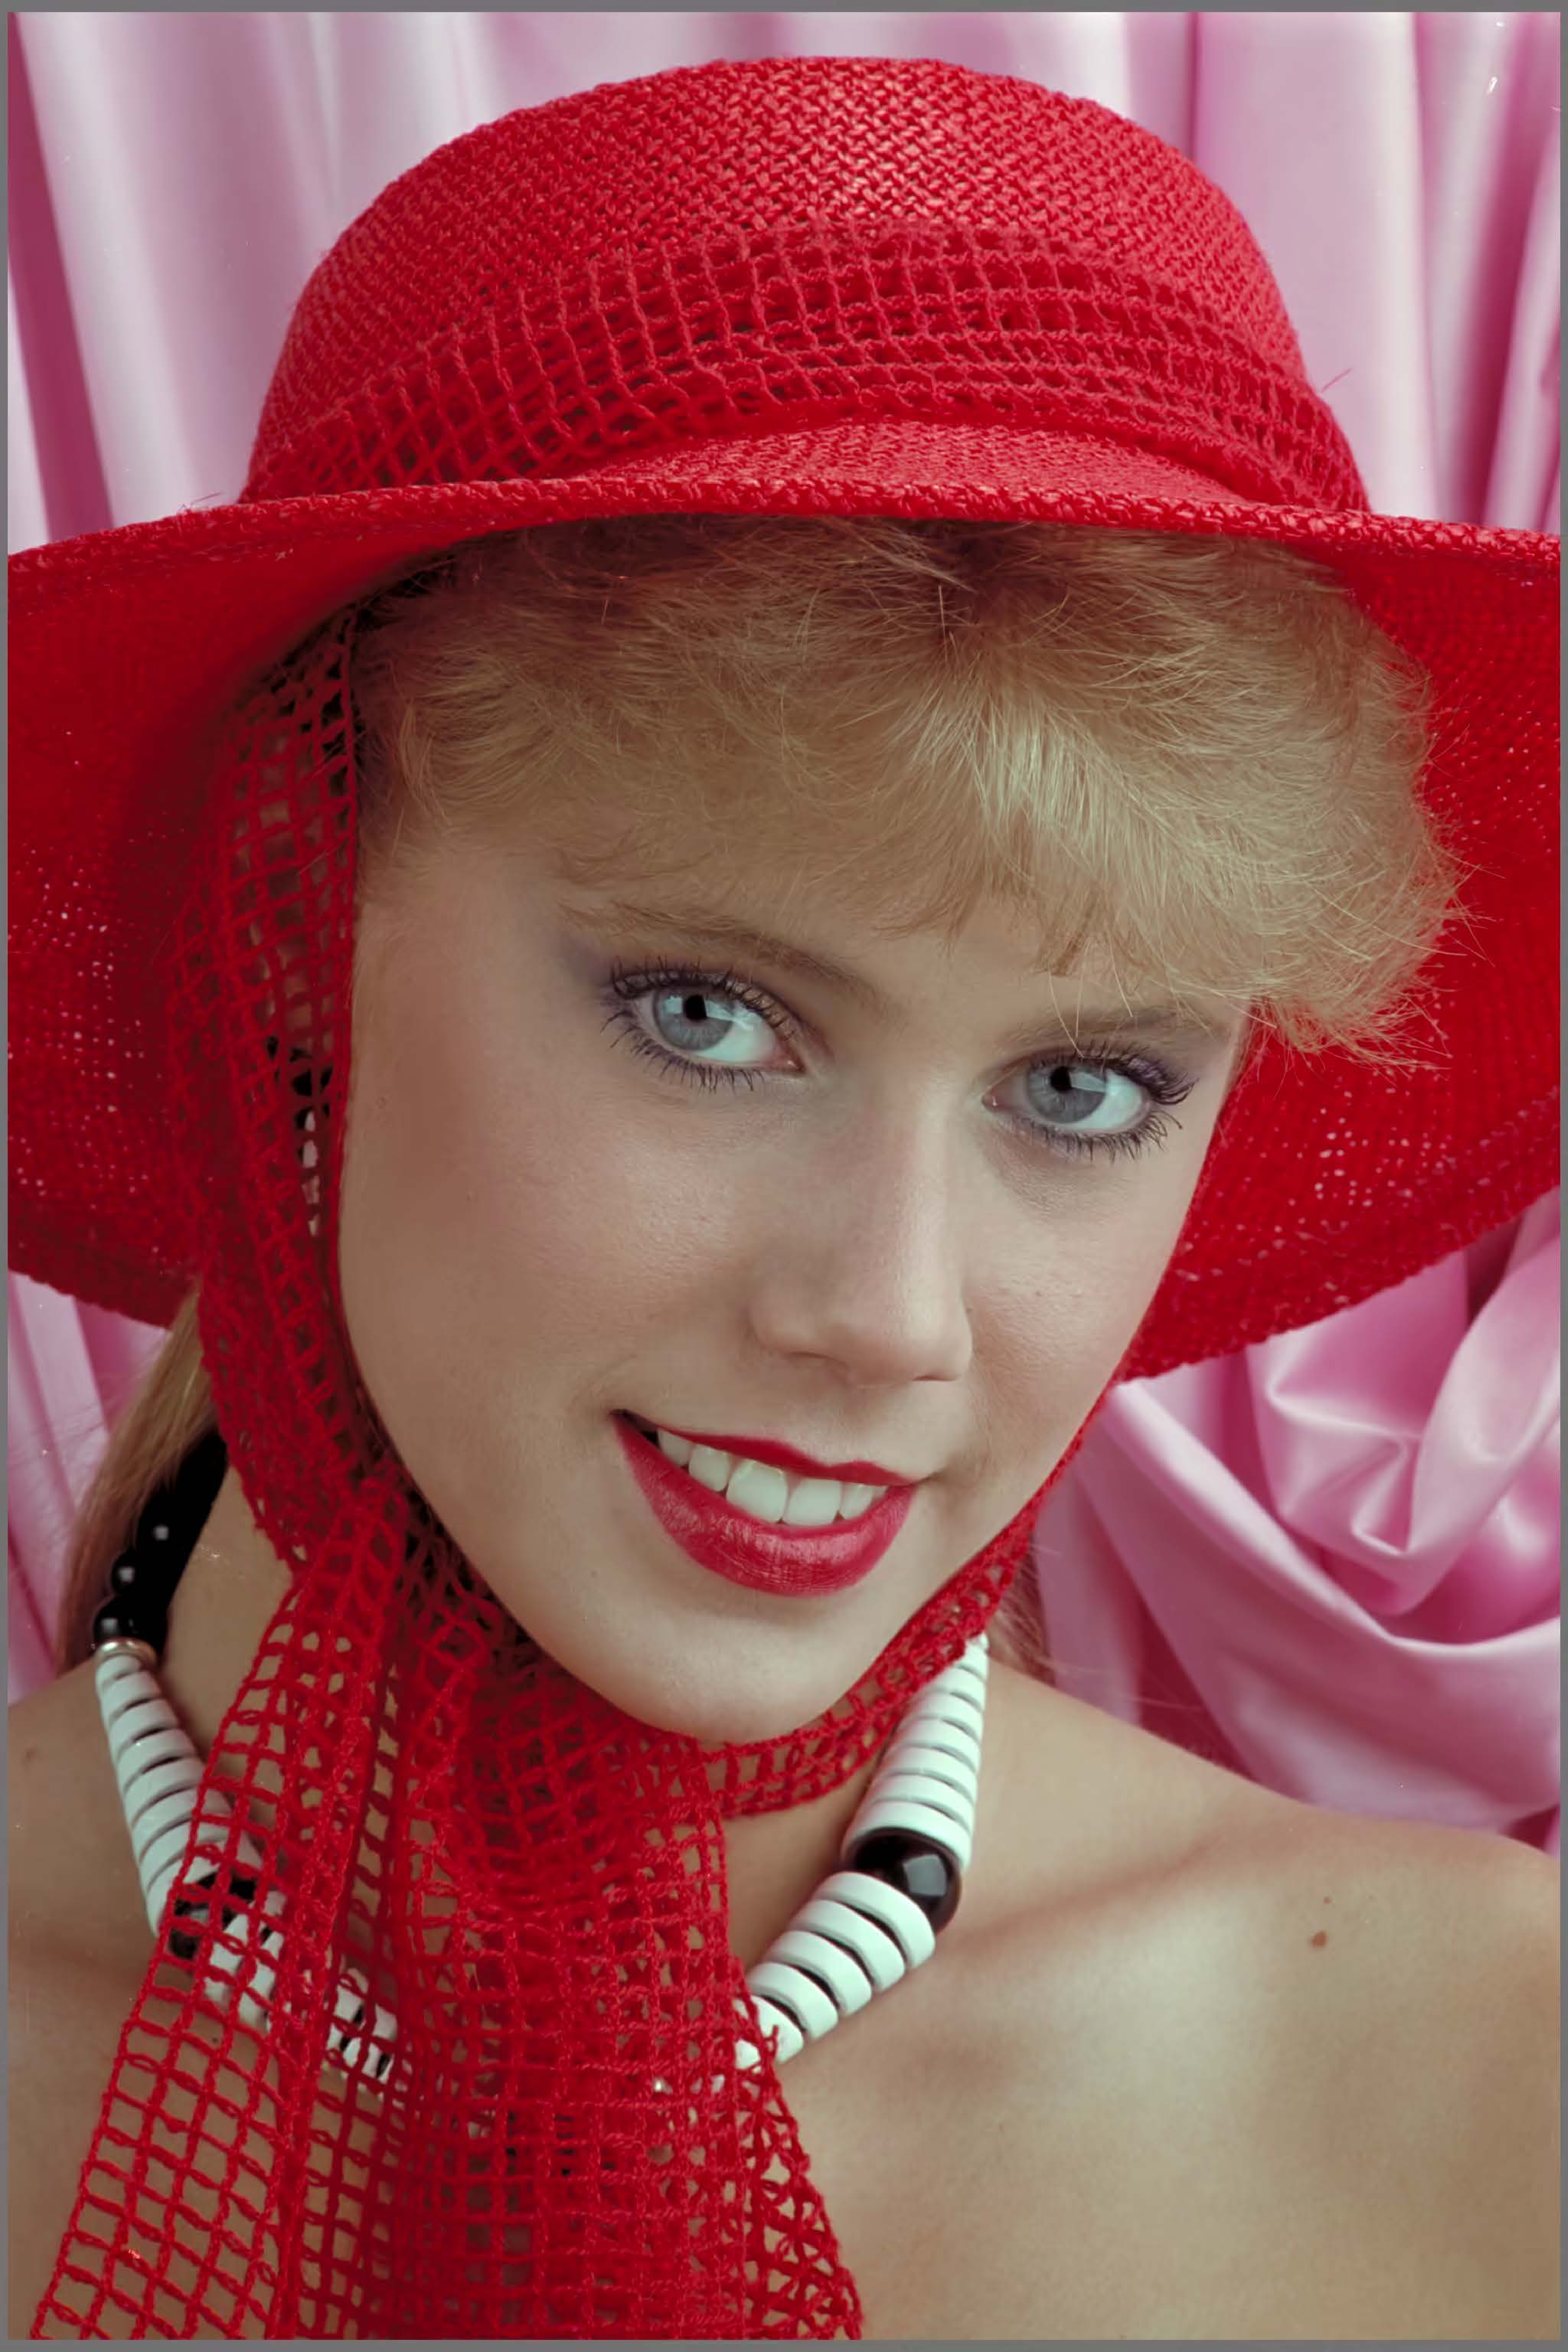
\includegraphics[width=\textwidth]{Immagini/IMAGES/VVC_2_IMG0004.pdf}
        \caption{VVC}
        \label{fig:CompressedVVC}
    \end{subfigure}
    \caption{Confronto PNG con VVC a 0.144 bpp}
    \label{fig:CompressionVVC}
\end{figure}
    \chapter{Metodi con intelligenza artificiale}
Negli ultimi anni abbiamo assistito ad uno sviluppo rapidissimo dell’intelligenza artificiale. Nonostante non sia una novità, i recenti avanzamenti tecnologici e la sempre più crescente diponibilità di dati di addestramento, hanno permesso lo sviluppo rapidissimo di queste tecnologie.\\
Anche l’ambito della computer vision e nello specifico della compressione ha seguito questo andamento, infatti negli ultimi anni sono state pubblicate numerose ricerche che vanno a proporre metodi sempre più efficienti per la compressione di immagini, appunto tramite l’uso di intelligenze artificiali.\\
Le immagini naturali contengono al loro interno molte ridondanze spaziali che possono essere sfruttate per comprimere senza diminuire la qualità percepita. Le reti neurali sono eccellenti per questo compito, in quanto permettono di ridurre di molto le ridondanze ed identificare le regioni più significative, in modo da operare con maggiore precisione su esse.
Partiamo quindi fornendo una rapida introduzione su cosa sia una rete neurale e quali sono i suoi componenti fondamentali.\\
Il componente fondamentale di una rete neurale è l’unita di elaborazione dati chiamata neurone, e più neuroni sono connessi tra di loro tramite connessioni pesate. Solitamente le reti sono composte da più livelli di neuroni e più livelli ci sono più si dice che la rete è profonda. L’analogia con la biologia umana non è casuale, infatti le reti neurali cercano di riprodurre la struttura interna del cervello umano per poterne emulare i processi cognitivi. \cite{sadeeq2021image}\\
Per rendere utilizzabile una rete non è sufficiente crearla definendone la struttura ed altri parametri come le funzioni di attivazione, l’algoritmo di ottimizzazione, il learning rate ed altri iper parametri, Ma va addestrata per il compito specifico per la quale la volgiamo utilizzare. Durante la fase di addestramento vengono aggiustati i pesi relativi alle connessioni tra i vari neuroni, questi pesi vengono modificati fino a quando viene trovata la migliore configurazione che permette di raggiungere il miglior risultato possibile nel compito che ci interessa.\\
Le reti neurali sono uno dei metodi più comunemente usati per compiti di regressione e classificazione \cite{sadeeq2021image}, il che le rende sfruttabili per cercare delle funzioni di regressione che permettano di comprimere le informazioni in delle loro rappresentazioni latenti più compresse.
Durante gli anni si sono sviluppate molte tipologie di reti neurali che si differenziano per configurazione o per metodo di addestramento, le strutture che vengono maggiormente utilizzate sono CNN, GAN e Autoencoder. Dei primi due metodi forniremo una breve descrizione per illustrarne le differenze principali, mentre sugli Autoencoder ci concentreremo maggiormente in quanto oggetto di questo studio.
Le reti neurali convoluzionali o CNN sono reti molto indicate per lavorare con immagini o video in quanto estraggono le caratteristiche dai dati di input tramite una serie di livelli convoluzionali e di pooling. Queste caratteristiche vengono poi utilizzate per operazioni di classificazione o identificazione.\\
Le reti avversarie generative o GAN vengono solitamente utilizzate per operazioni di generazione. Queste reti sono costituite da due parti, un generatore e un discriminatore. Il generatore cerca di generare, grazie a ciò che ha appreso dai dati di esempio, nuovi esempi il più realistici possibili per cercare di ingannare il discriminatore. Il discriminatore invece cerca di capire quali esempi sono reali e quali generati. 


\section{Funzionamento degli autoencoder}
Gli autoencoder o autocodficatori sono un modello, le cui prime applicazioni risalgono al 1980, che consiste di due parti. Un codificatore si occupa di effettuare l’embedding dell’input, ovvero convertire l’input in una sua rappresentazione latente di dimensione inferiore. Da questa rappresentazione la seconda parte, il decodificatore, cerca di ricostruire l’input nel modo più fedele possibile. Lo schema classico di un autoencoder è visibile nell’immagine \ref{fig:modelloAutoencoder}\\
Queste reti sono allenate utilizzando delle funzioni di perdita che vanno a misurare la differenza tra i dati in ingresso al codificatore e il prodotto del decodificatore. In base al risultato della funzione di perdita aggiustano i pesi delle reti fino a raggiungere il miglior risultato possibile, ovvero fino a realizzare una ricostruzione il più simile possibile ai dati di input.
Gli autoencoder non sono però sufficienti per costruire un algoritmo di compressione che, come illustrato precedentemente, consiste di almeno tre elementi e più recentemente quattro.
\newpage
\begin{figure}[!h]
    \centering
    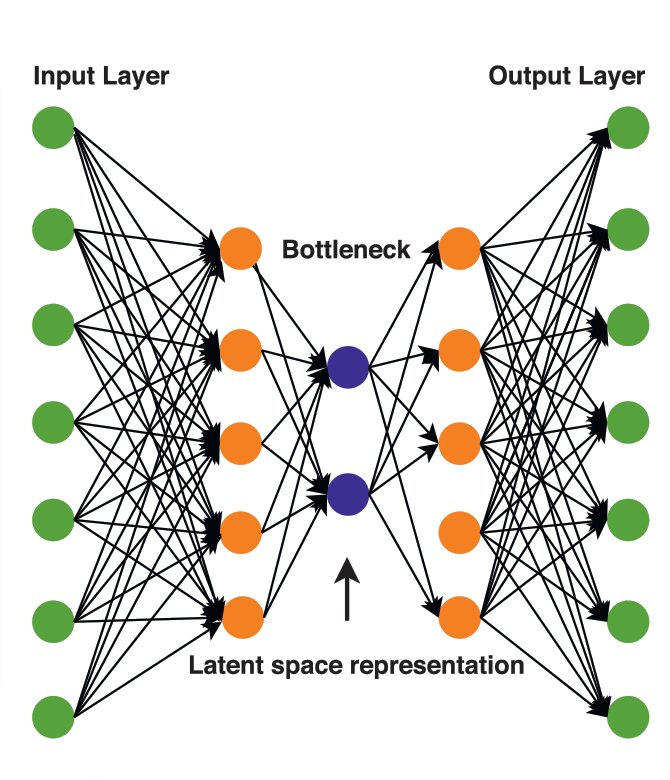
\includegraphics[width=0.5\textwidth]{Immagini/Autoencoder_scheme.png}
    \caption{Diagramma generico di un autoencoder}
    \label{fig:modelloAutoencoder}
\end{figure}
\section{Reti di Compressione}
Per ovviare a questo problema sono stati quindi sviluppati i Compressive AutoEncoder o CAE, che non sono nient’altro che un’estensione degli autoencoder in cui oltre alla rete neurale viene aggiunto un modello di probabilità che si occupa di assegnare un numero di bit alle rappresentazioni in base alla loro frequenza. Questa aggiunta permette di effettuare la codifica entropica della rappresentazione latente. \cite{theis2017lossy}\\
La funzione di perdita di questa nuova architettura \ref{eq:CAELoss} varia leggermente rispetto quella dei soli autoencoder, in quanto viene aggiunto un termine che tiene conto del numero di bit utilizzati. 
\begin{equation}\label{eq:CAELoss}
    L = \underbrace{- \log_{2}(Q([f(x)]))}_{\textrm{numero di bit}} + \beta \cdot \underbrace{d(x,g([f(x)]))}_{\textrm{distorsione}}
\end{equation}\\
Come possiamo vedere, l’equazione \ref{eq:CAELoss} consiste di due termini principali, il termine di destra rappresenta la distorsione tra ingresso e uscita della rete. Il secondo termine a sinistra viene introdotto appositamente per le CAE e stima il numero di bit utilizzati, questo permette di ottimizzare la rete non solo in base alla distorsione ma anche in base al numero di bit. Per controllare il compromesso tra numero di bit e distorsione viene introdotto il parametro $\beta$.\\
Il problema con questa nuova funzione nasce dal fatto che durante la fase di backpropagation, con tecniche come Stocastic Gradient Descent (SGD) dove è necessario calcolare il gradiente. La funzione \ref{eq:CAELoss} sopra illustrata non può essere utilizzata in quanto composta da funzioni non differenziabili, ovvero la funzione $Q$ e l’arrotondamento $[\bullet]$. Per ovviare a questo inconveniente è necessario trovare delle alternative differenziabili.\\
Theis et al. \cite{theis2017lossy} propone due soluzioni possibili, basate sul lavoro di Ballé et al. (2016) \cite{balle2018variational}. La prima soluzione si propone di risolvere il problema della funzione di arrotondamento, mentre Ballé et al. (2016) proponeva invece di utilizzare del rumore additivo gaussiano. \ref{eq:mbtGaussianNoise}.\\
\begin{equation}\label{eq:mbtGaussianNoise}
    [f(x)] \approx f(x) + u
\end{equation}\\
Theis propone invece di rimpiazzare la derivata durante la fase di backpropagation con una sua approssimazione lineare. Empiricamente hanno verificato che l'arrotondamento lineare $r(y)=y$ funziona alla pari di molte altre funzioni più elaborate.\\
La seconda soluzione risolve invece il problema della non differenziabilità della funzione di quantizzazione $Q$, utilizzando un’approssimazione continua \ref{eq:theisLinearApprox}.\\
\begin{equation}\label{eq:theisLinearApprox}
    Q(z) = \int_{[-.5,.5[^{M}} q(z+u) du
\end{equation}\\
In questa approssimazione $q$ rappresenta la densità di probabilità della distribuzione $Q$.\\
Lo sviluppo dei compressive autoencoder o CAE e le soluzioni proposte per rendere possibile l’esecuzione di algoritmi di addestramento, che richiedono il calcolo dei gradienti delle funzioni di perdita. Hanno permesso di sviluppare, negli anni successivi, modelli e nuove soluzioni in grado di ottenere buone prestazioni rispetto agli algoritmi tradizionali. Una lista che comprende tutti i metodi sviluppati fino al 2022 è presente nel lavoro di Mishra et al. \cite{mishra2022deep}, noi ci concentreremo sui tre che hanno fornito il maggiore contributo alla ricerca.


\subsection{Ballé 2018}
Il primo metodo che andiamo ad analizzare è quello proposto nel 2018 da Ballé et al. \cite{minnen2018joint} che prosegue il lavoro di Ballè et al. del 2016 \cite{balle2018variational}, lavoro che ha ispirato anche la soluzione sopra descritta offerta da Theis \ref{eq:theisLinearApprox} un anno prima.\\
Il metodo proposto da Ballé et al. nel 2018 utilizza un modello di probabilità misto a scala gaussiana o GSM dove i parametri di scala sono condizionati da un iperparametro. Questo modello permette l’addestramento end-to-end, ciò include anche l’ottimizzazione della rappresentazione quantizzata dell’iper parametro, del modello dell’entropia e dell’autoencoder principale.\\
L’innovazione principale che questo modello porta è l’aggiunta dell’iper parametro compresso nell’informazione trasmessa, ciò permette al decodificatore di usare un modello dell’entropia condizionato dall’iper parametro. Questo consente di avere un modello per l’entropia dipendente dall’immagine.\\
L’immagine \ref{fig:balle2018Network} mostra l’architettura ad alto livello del modello di compressione, come si può osservare il modello sia composto da due sottoreti.
\begin{figure}[!h]
    \centering
    \includegraphics[width=0.5\textwidth]{Immagini/Ballé2018_Rete.png}
    \caption{Diagramma rete Ballè 2018 et al., immagine presa dal documento \cite{minnen2018joint}}
    \label{fig:balle2018Network}
\end{figure}\\
La prima sottorete è l’autoencoder principale che ricava una rappresentazione latente delle immagini. La seconda invece ricava un modello di probabilità per effettuare la codifica entropica della rappresentazione latente.\\
I dati provenienti dalle due sottoreti vengono combinati dalla rete per i parametri dell’entropia, generando la media e la scala per il modello gaussiano dell’entropia.\\
La funzione di perdita utilizzata da questo modello \ref{eq:mbtLoss1} è molto simile a quella riportata in precedenza per i CAE, dove il parametro $\beta$ viene sostituito dal moltiplicatore di Lagrange $\lambda$ che regola il compromesso tasso-distorsione. Come di consueto l’obbiettivo di addestramento è quello di minimizzare la funzione di perdita rispetto ai parametri del modello.\\
\begin{equation}\label{eq:mbtLoss1}
    R + \lambda \cdot D = \underbrace{\mathbb{E}_{x \sim p_{x}}[-\log_{2} p_{\hat{y}}(\lfloor f(x) \rceil)]}_{\textrm{numero di bit}} + \lambda \cdot \underbrace{\mathbb{E}_{x \sim p_{x}}[d(x,g(\lfloor f(x) \rceil))]}_{\textrm{distorsione}}
\end{equation}\\
L’entropia di ogni rappresentazione latente $\hat{y_{i}}$ viene modellata come una gaussiana convoluta con una distribuzione uniforme, dunque il modello dell’entropia ha la formulazione \ref{eq:mbtEntropy}.
\begin{equation}\label{eq:mbtEntropy}
    p_{\hat{y}}(\hat{y}|\hat{z}) = \prod_{i}(\mathcal{N}(\mu_{i},\sigma_{i}^{2})*\mathcal{U}(-\tfrac{1}{2},\tfrac{1}{2}))(\hat{y_{i}})
\end{equation}\\
Per predire media e scala della gaussiana invece vengono utilizzati sia l’iper distribuzione $\hat{z}$, sia il contesto della rappresentazione latente $\hat{y}$.
In questo modello ci aspettiamo che l’iper codificatore e l’iper decodificatore apprendano due funzioni leggermente differenti in quanto lavorano in combinazione con una rete autoregressiva che determina i parametri del modello dell’entropia. Ed essendo sia la rappresentazione latente che la iper-latente parte dell’informazione compressa generata dalla rete, l’equazione \ref{eq:mbtLoss1} deve essere leggermente espansa nell' equazione \ref{eq:mbtLoss2}, per includere il costo di codifica degli iper-latenti e utilizzare come distorsione la distanza quadratica media.\\
\begin{equation}\label{eq:mbtLoss2}
    R + \lambda \cdot D = \underbrace{\mathbb{E}_{x \sim p_{x}}[-\log_{2} p_{\hat{y}}(\hat{y})]}_{\textrm{bit(latenti)}} + \underbrace{\mathbb{E}_{x \sim p_{x}}[-\log_{2} p_{\hat{z}}(\hat{z})]}_{\textrm{bit(iper latenti)}} + \lambda \cdot \underbrace{\mathbb{E}_{x \sim p_{x}}||x-\hat{x}||_{2}^{2}}_{\textrm{distorsione}}
\end{equation}\\
Il team di Ballé fornisce anche i dettagli implementativi per i livelli della rete, che abbiamo riportato nella tabella \ref{tab:mbtLayers}.
\begin{table}[!h]
    \centering
    \resizebox{\textwidth}{!}{%
    \begin{tabular}{@{}c|c|c|c|c|c@{}}
    Codificatore & Decodificatoree & \begin{tabular}[c]{@{}c@{}}Iper\\ Codificatore\end{tabular} & \begin{tabular}[c]{@{}c@{}}Iper\\ Decodificatore\end{tabular} & \begin{tabular}[c]{@{}c@{}}Predittore di\\ Contesto\end{tabular} & \begin{tabular}[c]{@{}c@{}}Parametri\\ Entropia\end{tabular} \\ \midrule
    Conv: 5x5 c192 s2 & Deconv: 5x5 c192 s2 & Conv: 3x3 c192 s1 & Deconv: 5x5 c192 s2 & Masked: 5x5 c384 s1 & Conv: 1x1 c640 s1 \\
    GDN & IGDN & Leaky ReLU & Leaky ReLU &  & Leaky ReLU \\
    Conv: 5x5 c192 s2 & Deconv: 5x5 c192 s2 & Conv: 5x5 c192 s2 & Deconv: 5x5 c288 s2 &  & Conv: 1x1 c512 s1 \\
    GDN & IGDN & Leaky ReLU & Leaky ReLU &  & Leaky ReLU \\
    Conv: 5x5 c192 s2 & Deconv: 5x5 c192 s2 & Conv: 5x5 c192 s2 & Deconv: 3x3 c384 s1 &  & Conv: 1x1 c384 s1 \\
    GDN & IGDN &  &  &  &  \\
    Conv: 5x5 c192 s2 & Deconv: 5x5 c3 s2 &  &  &  & 
    \end{tabular}%
    }
    \caption{Ad ogni riga della tabella corrisponde un livello del modello generalizzato, i dati della tabella sono stati ricavati dal documento  \cite{minnen2018joint}}
    \label{tab:mbtLayers}
\end{table}\\
Possiamo vedere degli esempi di compressione con questa rete nelle immagini \ref{fig:CompressedMbt2018} e \ref{fig:CompressedMbt2018Mean}, le due immagini sono state prodotte da due versioni diverse della rete, rispettivamente con media della gaussiana variabile e con media della gaussiana fissata a zero.\\
    

\subsection{Cheng 2020}
Il secondo metodo che approfondiremo è quello proposto da Cheng et al. nel 2020 \cite{cheng2020learned}, questo metodo prende come punto di partenza il lavoro di Ballè et al. \cite{minnen2018joint} e lo migliora apportando delle modifiche al modello di probabilità delle rappresentazioni latenti.\\
Il lavoro di Ballè et al. \cite{minnen2018joint} utilizza una distribuzione Gaussiana con media e scala congiunta con un modello autoregressivo \ref{eq:mbtEntropy}. I test svolti dal team di Cheng hanno evidenziato della ridondanza spaziale residua, ridondanza che se possibile eliminare porterebbe a rappresentazioni leggermente ridotte e quindi più efficienti.\\
La loro proposta è quindi quella di utilizzare una miscela di gaussiane con la formulzione \ref{eq:cheng2020Entropy}
\begin{equation}\label{eq:cheng2020Entropy}
    p_{\hat{y}}(\hat{y}|\hat{z}) = (\sum_{k=1}^{K} w_{i}^{(k)} \mathcal{N}(\mu_{i}^{(k)},\sigma_{i}^{2(k)})*\mathcal{U}(-\tfrac{1}{2},\tfrac{1}{2}))(\hat{y_{i}})
\end{equation}\\
Quindi ogni miscela è caratterizzata da tre parametri, un peso $w_{i}^{(k)}$, la media $\mu_{i}^{(k)}$ e la scala $\sigma_{i}^{2(k)}$.
Con questo metodo sono comunque presenti delle ridondanze, ma l’aggiunta dei pesi $w_{i}$ permette al modello di adattarsi alle diverse regioni delle immagini. Inoltre le scale prodotte con questo metodo sono più piccole rispetto al metodo di Ballè et al. \cite{minnen2018joint}, il che rende il modello più accurato, risultando in una rappresentazione compressa dell’immagine che richiede meno bit.\\
L’architettura della rete proposta da Cheng et al. \cite{cheng2020learned} è rappresentata nell’immagine \ref{fig:cheng2020Network}, come possiamo osservare anche qui sono presenti due sottoreti. Una responsabile di ricavare la rappresentazione latente dell’immagine, l’altra di ricavare gli iperparametri.\\
\begin{figure}[!h]
    \centering
    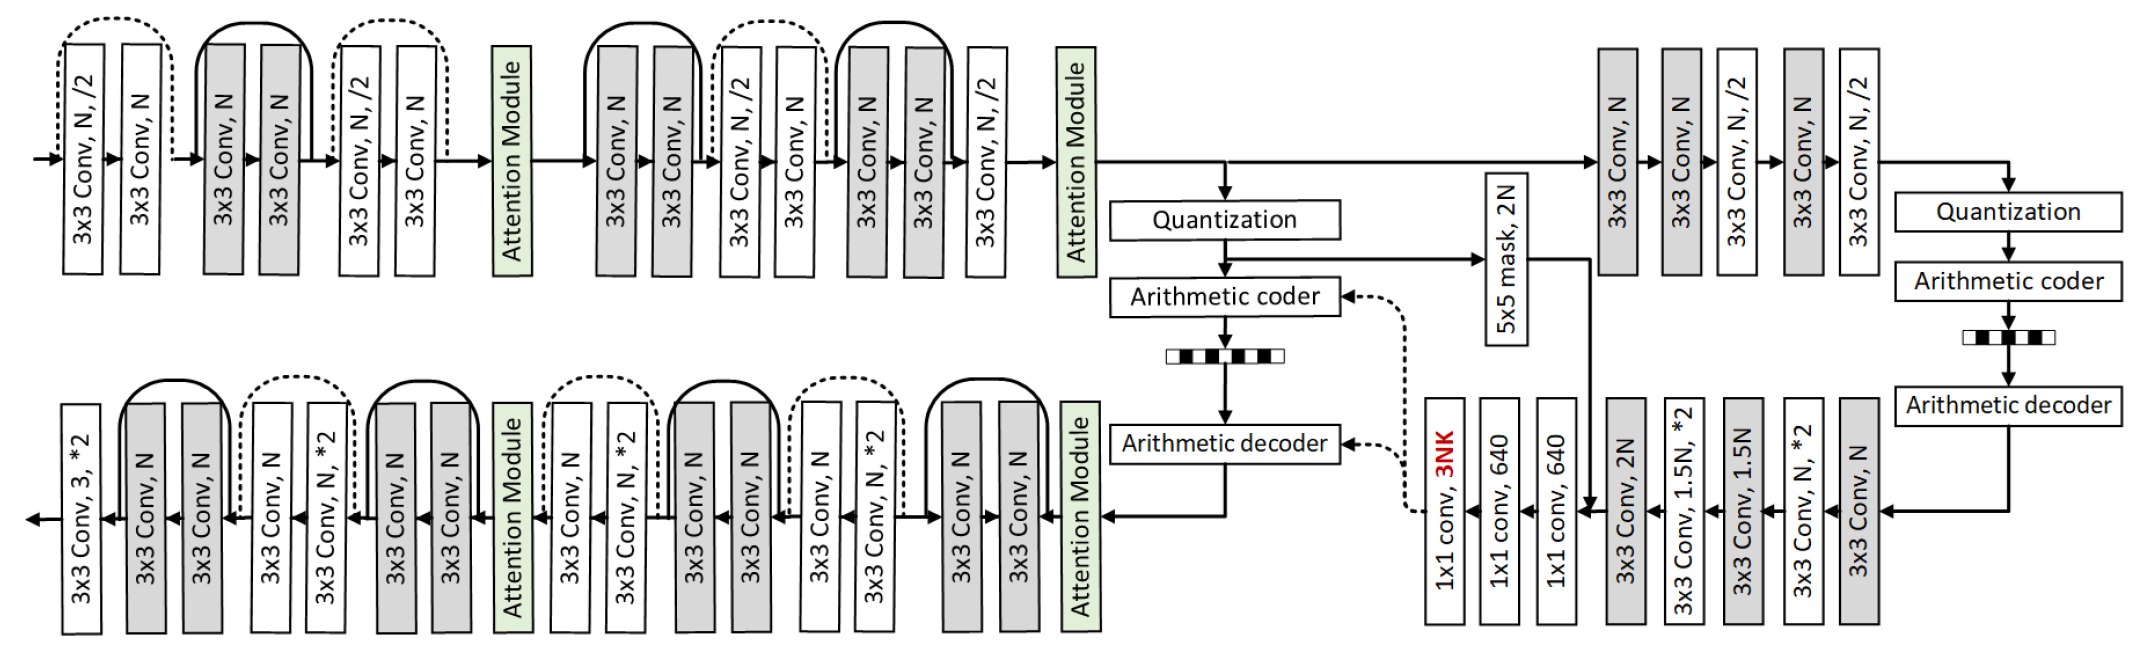
\includegraphics[width=0.9\textwidth]{Immagini/Cheng2020_Rete.png}
    \caption{Diagramma rete Cheng 2020 et al., immagine presa dal documento \cite{cheng2020learned}}
    \label{fig:cheng2020Network}
\end{figure}\\
Questo modello introduce due nuovi moduli, gli Attention Module, questi servono per aiutare la rete a prestare maggiore attenzione alle parti più complesse delle immagini e ridurre i bit necessari per rappresentare invece le parti più semplici. Uno schema che illustra il funzionamento di un attention module è visibile nell’immagine \ref{fig:cheng2020AttnModuleA}.\\
Questi moduli però richiedono una grande quantità di tempo in fase di addestramento, per cercare di ovviare a questo problema viene proposta una versione semplificata \ref{fig:cheng2020AttnModuleB} in cui è stato rimosso il blocco contenente le informazioni non locali.\\
Possiamo vedere degli esempi di compressione con questa rete nelle immagini \ref{fig:CompressedCheng2020} e \ref{fig:CompressedCheng2020Attention}, le due immagini sono state prodotte da due versioni diverse della rete, rispettivamente senza Attention module e con.\\
\newpage
\begin{figure}[h!]
    \centering
    \begin{subfigure}[]{0.6\textwidth}
        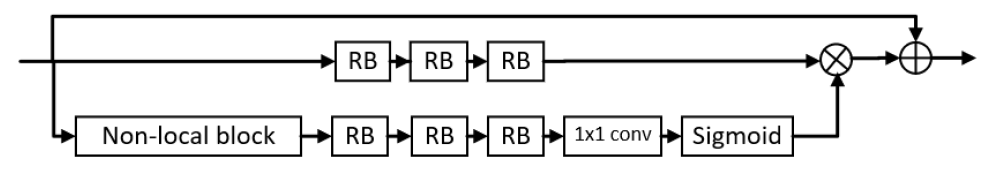
\includegraphics[width=\textwidth]{Immagini/Cheng2020_AttnModuleA.png}
        \caption{Attention module completo}
        \label{fig:cheng2020AttnModuleA}
    \end{subfigure}
    \vspace*{1.5cm}
    \begin{subfigure}[]{0.6\textwidth}
        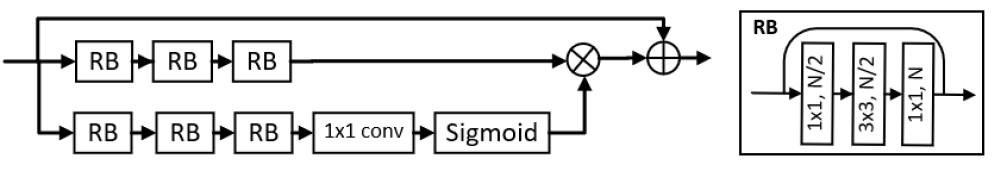
\includegraphics[width=\textwidth]{Immagini/Cheng2020_AttnModuleB.png}
        \caption{Attention module semplificato}
        \label{fig:cheng2020AttnModuleB}
    \end{subfigure}
    \caption{Varianti degli attention modules sviluppati da Cheng 2020 et al., immagine presa dal documento \cite{cheng2020learned}}
    \label{fig:cheng2020AttnModule}
\end{figure}

\subsection{Wang 2022}
Il terzo ed ultimo metodo che andremo ad approfondire è quello proposto nel 2022 da Wang et al. \cite{wang2022neural}, questo metodo propone un nuovo approccio per rendere la compressione di un’immagine dipendente dall’immagine stessa. Per fare ciò hanno preso ispirazione dai precedenti lavori e dai modelli di codifica ibridi, il framework proposto cerca la migliore trasformata per comprimere l’immagine specifica, la proposta di Wang et al. si differenzia dai metodi sviluppati in precedenza nei seguenti aspetti.\\
Durante la fase di codifica vengono prodotti sia la rappresentazione compressa sia una rappresentazione neuro-sintattica, in grado di catturare informazioni astratte sul contesto dell’immagine che possano aiutare a proiettare la rappresentazione compressa in un sottospazio in cui i coefficienti sono più compatti.\\
Il modello per la codifica entropica si differenzia da quelli esistenti in quanto le due rappresentazioni latenti $\hat{z_{s}}$ e $\hat{z_ {c}}$ vengono codificate separatamente \ref{eq:wang2022LatentEnc} in due stringhe di bit compresse $b_{s}$ e $b_{c}$.\\
\begin{equation}\label{eq:wang2022LatentEnc}
    b_{c} = EC (\hat{z_{c}}), \hspace{1 cm} b_{s} =  EC (\hat{z_{s}})
\end{equation}\\
La compressione separata permette un controllo più preciso del processo di codifica.\\
Simmetricamente, avviene il processo di decodifica \ref{eq:wang2022LatentDec}.\\
\begin{equation}\label{eq:wang2022LatentDec}
    \hat{z_{c}} =  ED (b_{c}), \hspace{1 cm} \hat{z_{s}} =  ED (b_{s}) 
\end{equation}\\
La funzione di decodifica proposta è dipendente dai dati, in quanto per immagini di input diverse $x$ si ottengono diverse rappresentazioni neuro-sintattiche $\hat{z_ {s}}$, in modo da generare trasformate di decodifica più specifiche.\\
La funzione di perdita che deve quindi essere ottimizzata in fase di addestramento della rete ha la struttura \ref{eq:wang2022Loss}. Dove $D$ rappresenta la metrica di distorsione, $R$ misura il bit-rate, $\hat{z_{h}}$ rappresenta l’iper distribuzione di $\hat{z_{s}}$ e $\hat{z_{c}}$, mentre $\lambda$ è l’iper parametro che regola il compromesso tra tasso di codifica e distorsione.\\
\begin{equation}\label{eq:wang2022Loss}
    L = D(x,\hat{x}) + \lambda (R(\hat{z_{c}}) +  R(\hat{z_{s}}) + R(\hat{z_{h}}))
\end{equation}\\
La struttura del modello proposto da Wang et al. è visibile nell’immagine \ref{fig:Wang2022Network}, come è possibile osservare ritroviamo la solita struttura composta da due sottoreti, una per di ricavare la rappresentazione latente dell’immagine, l’altra per ricavare gli iperparametri. La novità introdotta in questo modello è la presenza di una trasformata dipendente dai dati in ingresso, questa capacità della rete corrisponde al percorso evidenziato in rosso all’interno della figura \ref{fig:Wang2022Network}.\\
\begin{figure}[!h]
    \centering
    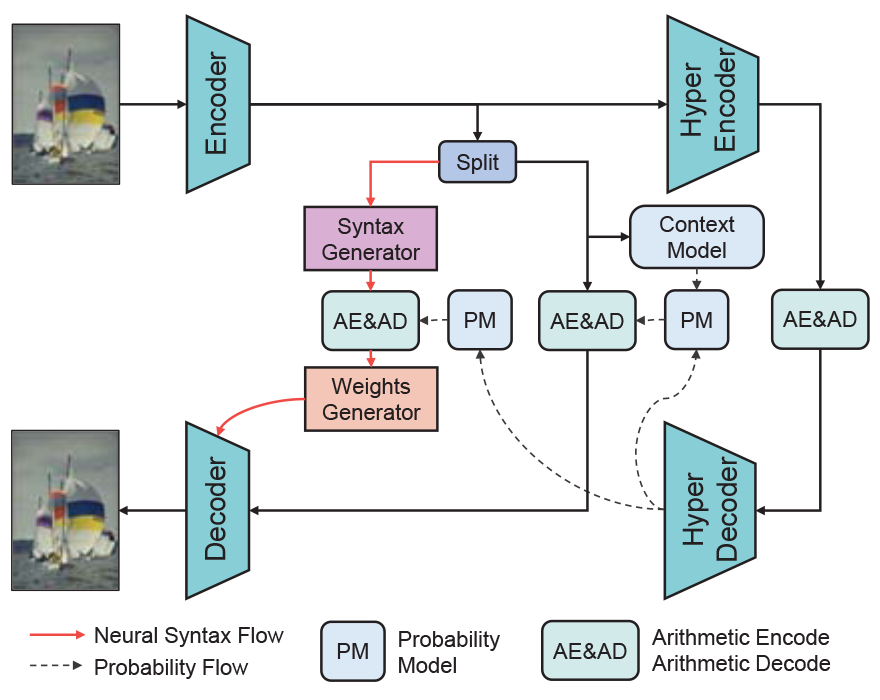
\includegraphics[width=0.6\textwidth]{Immagini/Wang2022_Rete.png}
    \caption{Diagramma rete Wang 2022 et al., immagine presa dal documento \cite{wang2022neural}}
    \label{fig:Wang2022Network}
\end{figure}\\
In questo modello vengono introdotti due nuovi moduli, un Syntax Generator e un Weights Generator di cui possiamo osservare una rappresentazione nelle immagini \ref{fig:Wang2022SyntaxGenerator} e \ref{fig:Wang2022WeightsGenerator}.\\
Il modulo di Syntax Generation \ref{fig:Wang2022SyntaxGenerator} è stato creato per estrarre delle informazioni di sintassi dall’input in fase di codifica, dopo averle estratte queste informazioni vengono mappate in un vettore unidimensionale $\hat{z_{s}}$ con un operazione di pooling globale. I vettori $\hat{z_{s}}$ vengono quindi concatenati, quantizzati e codificati.\\
\begin{figure}[h!]
    \centering
    \begin{subfigure}[]{0.4\textwidth}
        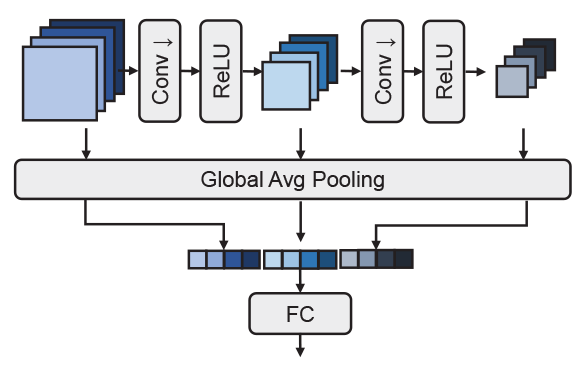
\includegraphics[width=\textwidth]{Immagini/Wang2022_SyntaxGenerator.png}
        \caption{Syntax Generator}
        \label{fig:Wang2022SyntaxGenerator}
    \end{subfigure}
    \hspace*{1 cm}
    \begin{subfigure}[]{0.4\textwidth}
        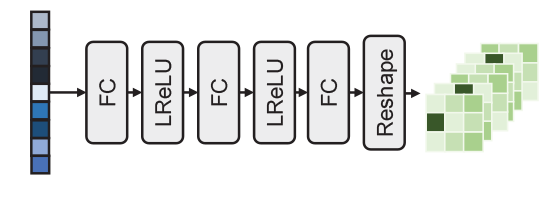
\includegraphics[width=\textwidth]{Immagini/Wang2022_WeightsGenerator.png}
        \caption{Weights Generator}
        \label{fig:Wang2022WeightsGenerator}
    \end{subfigure}
    \caption{Moduli aggiuntivi creati dal tem di Wang et al. per il loro modello, immagini prese dal documento \cite{wang2022neural}}
    \label{fig:Wang2022Modules}
\end{figure}
Il secondo modulo \ref{fig:Wang2022WeightsGenerator} si occupa invece di mappare la rappresentazione neuro-sintattica $\hat{z_{s}}$, ottenuta durante la codifica, in parametri per i kernel della rete di decodifica, l’estrazione di questi parametri è quello che permette a questa rete di creare delle trasformate dipendenti dai dati.\\
Questi parametri vengono utilizzati dalla rete di decodifica, come possiamo vedere nella figura \ref{fig:Wang2022Convolution}, in quanto solo i parametri dell’ultimo livello della rete sono fissati, mentre quelli dei livelli precedenti vengono generati dal Weights Generator, in modo da permettere alla rete di adattarsi ad immagini diverse.\\
\begin{figure}[!h]
    \centering
    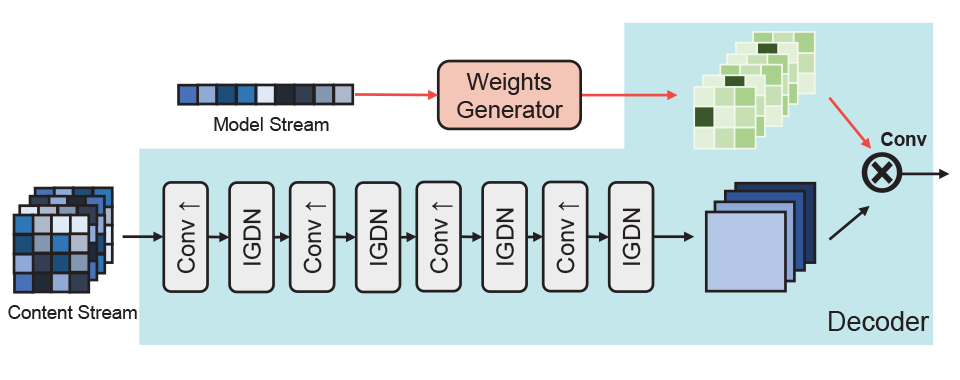
\includegraphics[width=0.5\textwidth]{Immagini/Wang2022_Convolution.png}
    \caption{Convoluzione di pesi e dati nel processo di decodifica nella rete Wang 2022, immagine presa dal documento \cite{wang2022neural}}
    \label{fig:Wang2022Convolution}
\end{figure}\\
Il team di Wang et al. ha inoltre sviluppato un modulo aggiuntivo di post-processing, utile per i casi in cui è richiesta una ricostruzione più dettagliata, anche questa rete fa uso della rappresentazione neuro-sintattica per adattarsi maggiormente alle varie immagini. Grazie a questa aggiunta il team di Wang et al. ha riportato di aver superato anche il codec VVC, che attualmente rappresenta lo stato dell’arte per la compressione di immagini.\\
Di questo modello non possiamo fornire degli esempi di compressione in quanto il team di Wang et al. \cite{wang2022neural} ha rilasciato il modello ma non la rete pre allenata e non avendo a disposizione dell'equipaggiamento adeguato per eseguire l'allenamento del modello, ci è stato impossibile utilizzare questa rete nei nostri esperimenti.\\
\newpage

\begin{figure}[t!]
    \centering
    \begin{subfigure}[]{0.25\textwidth}
        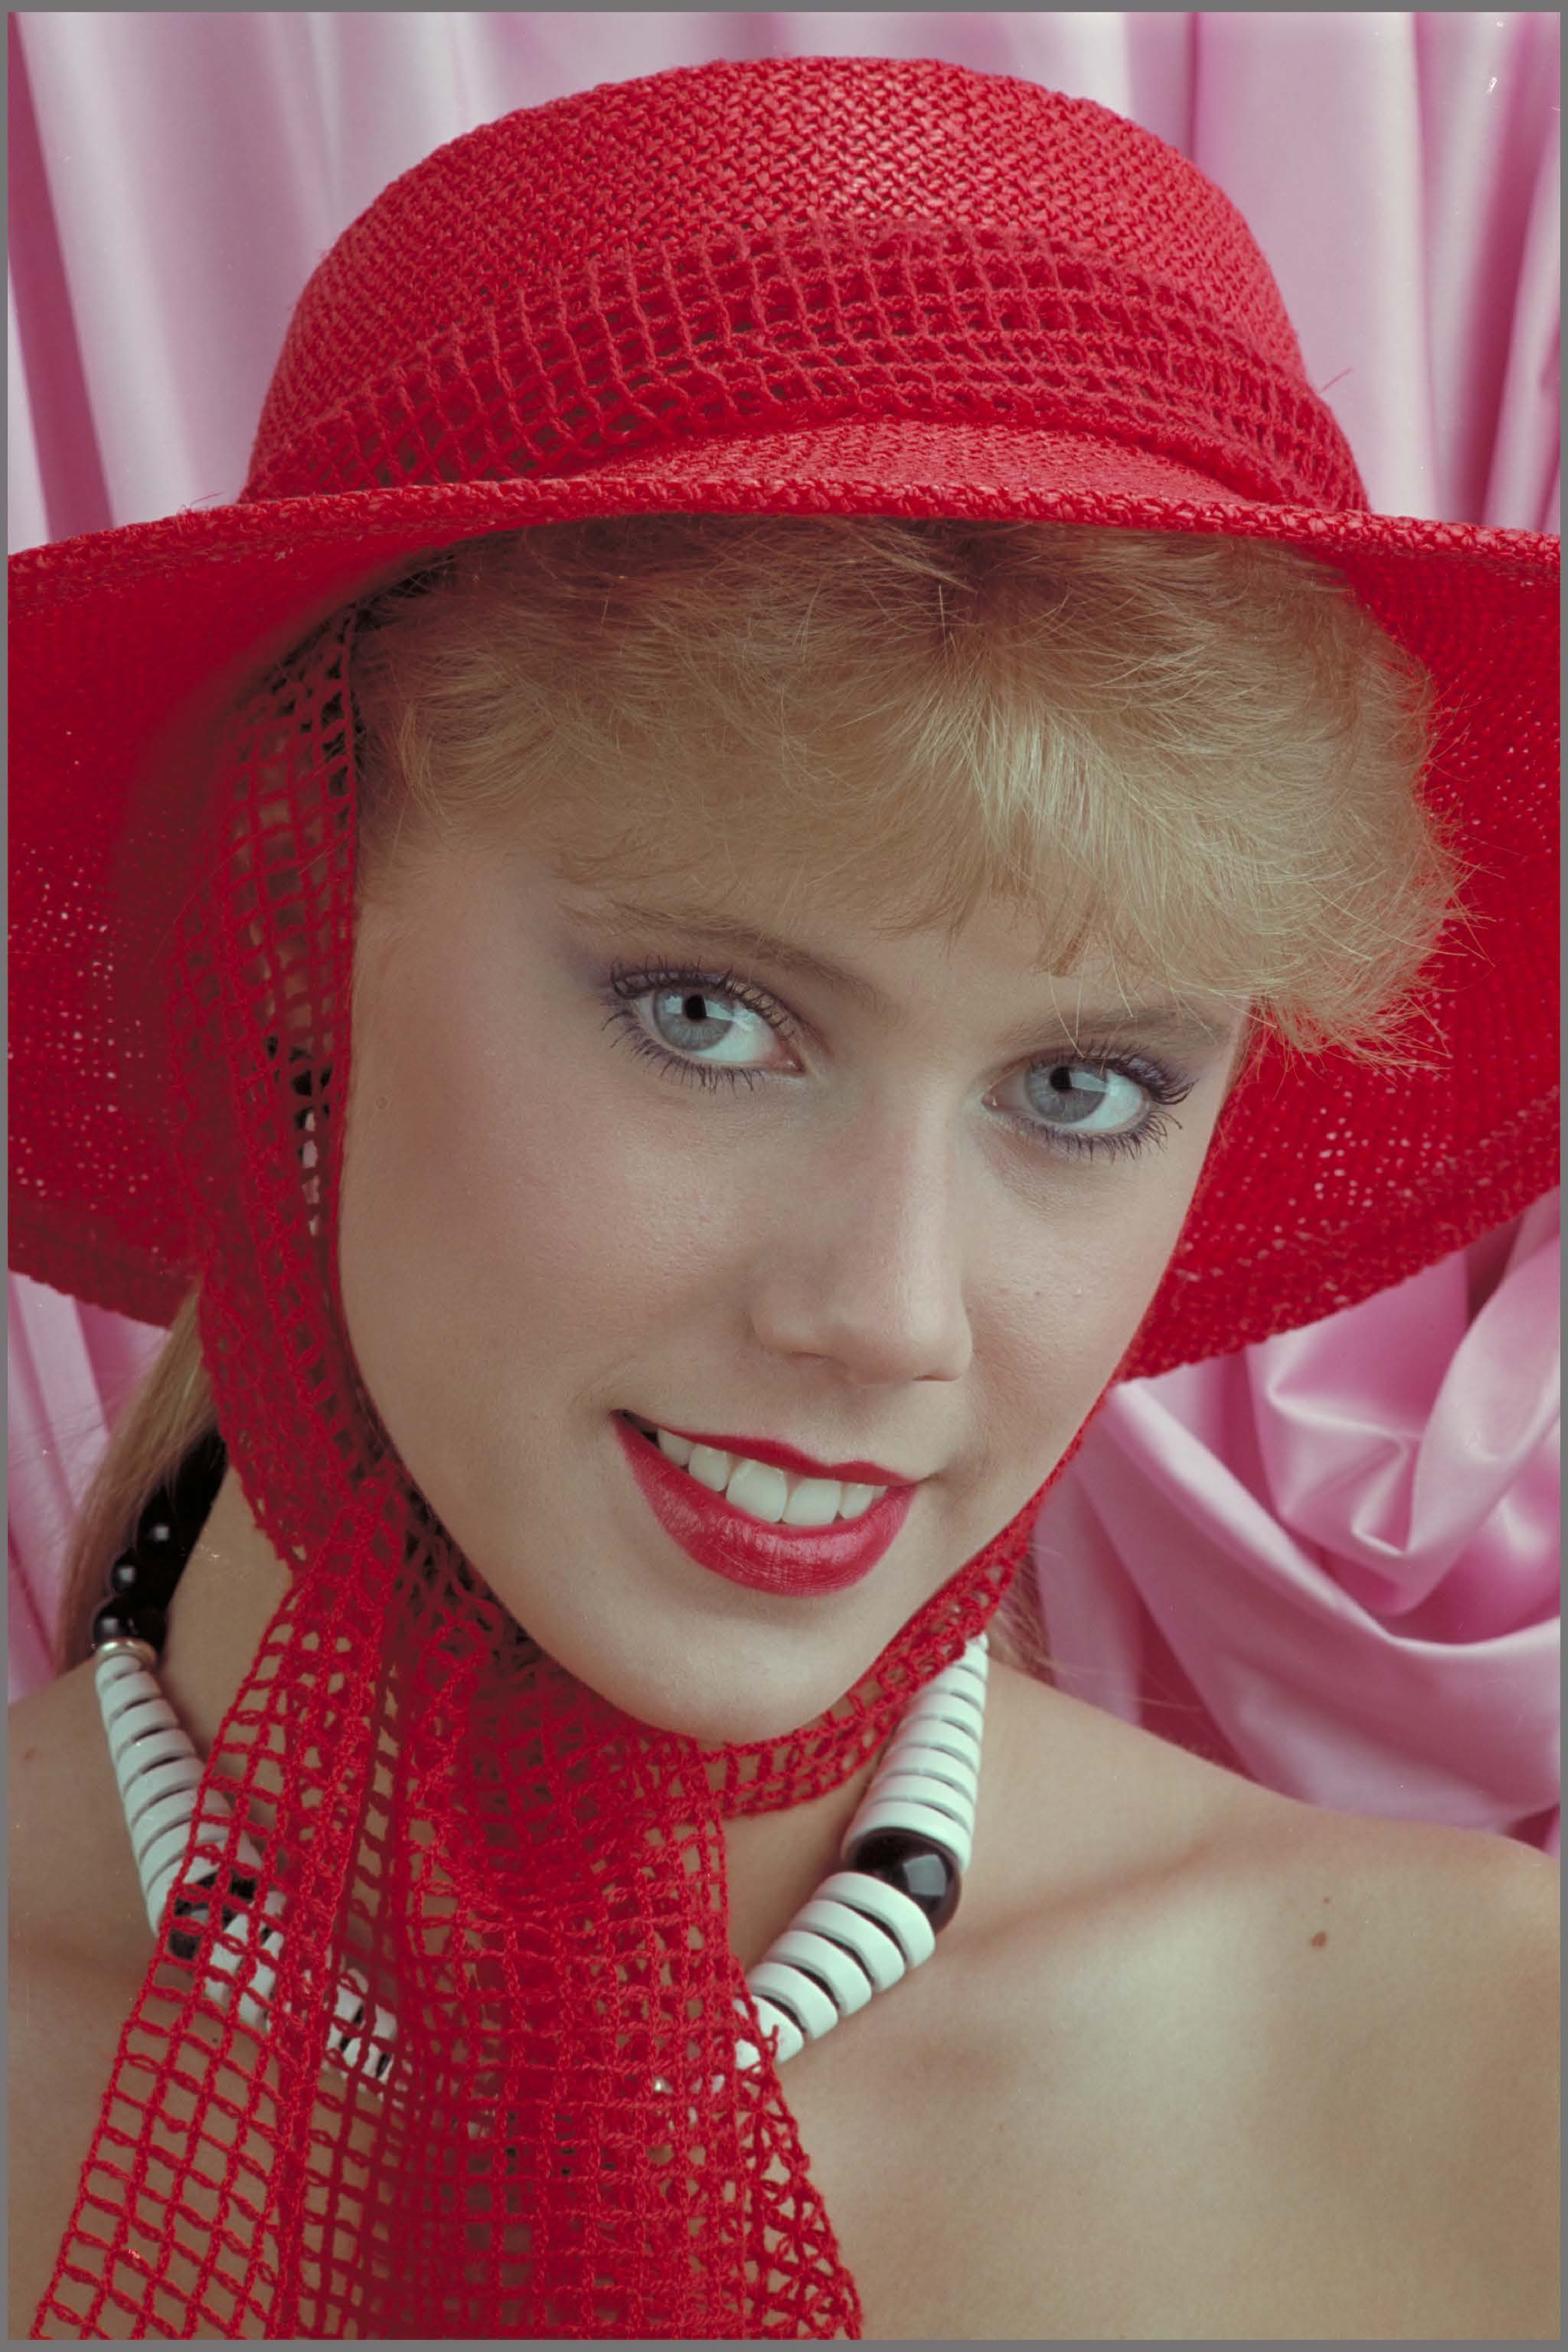
\includegraphics[width=\textwidth]{Immagini/IMAGES/PNG_IMG0004.pdf}
        \caption{Originale}
        \label{fig:OriginalMbt2018}
    \end{subfigure}
    \hspace{0.5cm}
    \begin{subfigure}[]{0.25\textwidth}
        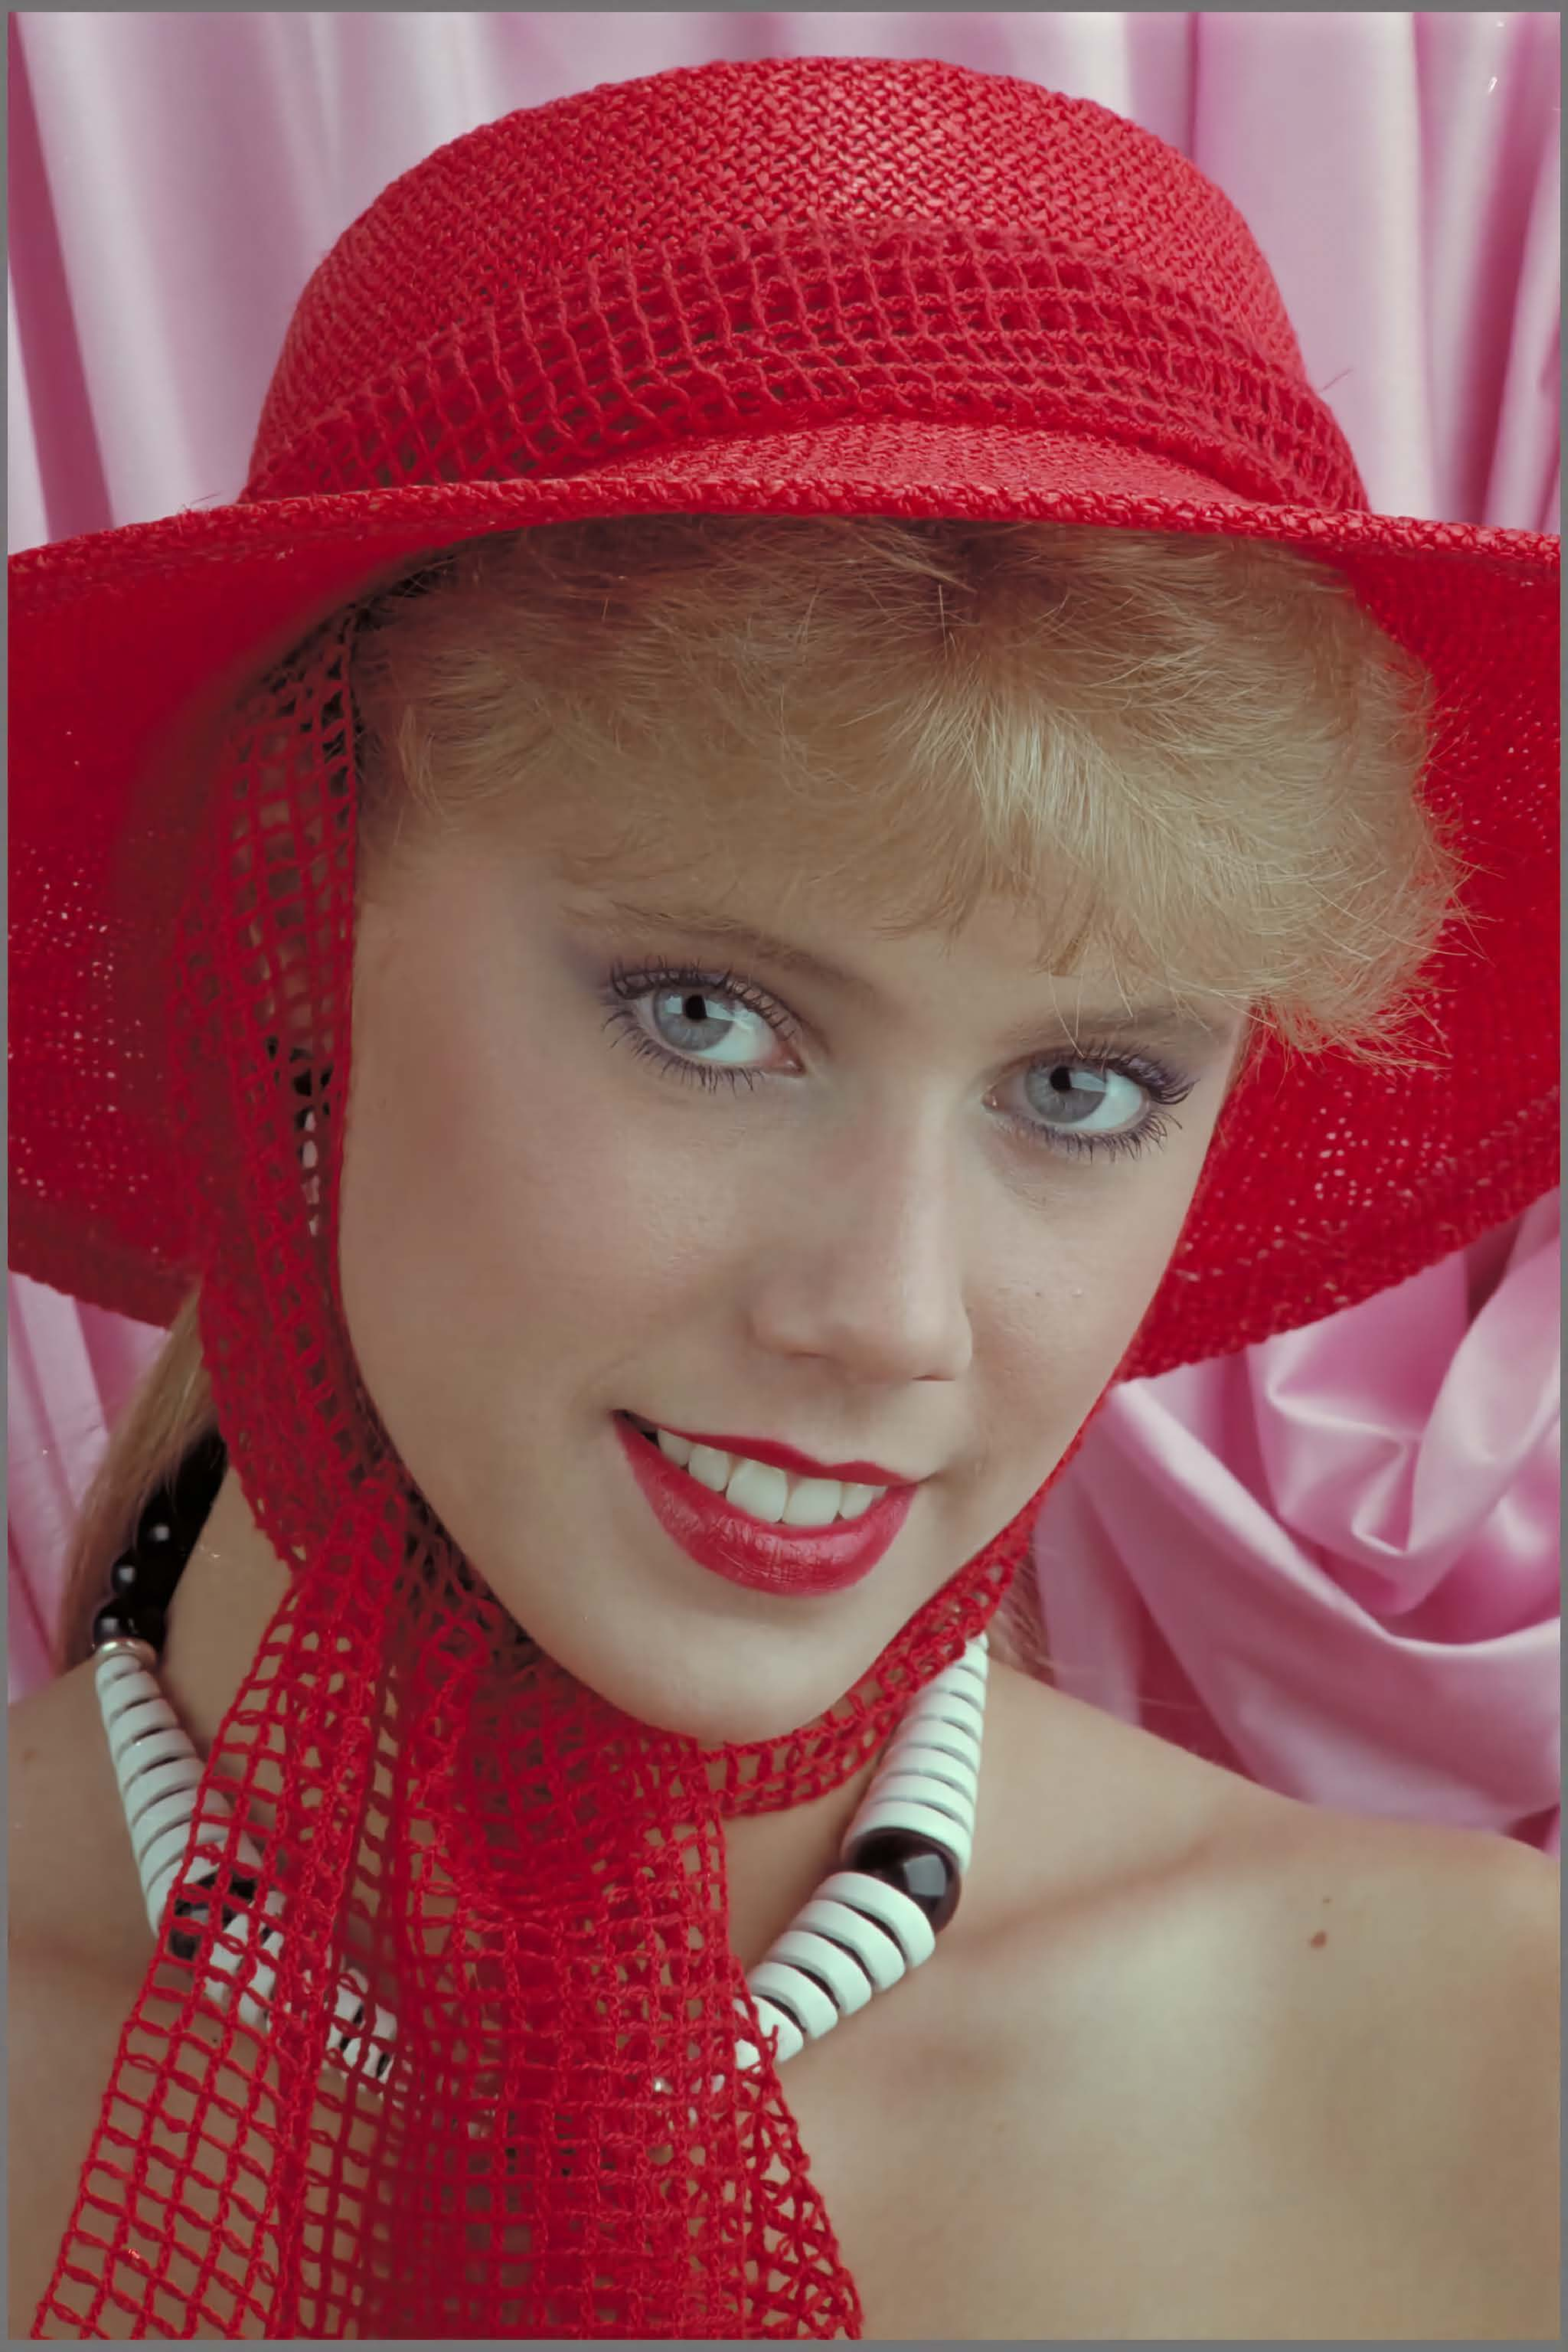
\includegraphics[width=\textwidth]{Immagini/IMAGES/mbt2018_3_IMG0004.pdf}
        \caption{mbt2018}
        \label{fig:CompressedMbt2018}
    \end{subfigure}
    \hspace{0.5cm}
    \begin{subfigure}[]{0.25\textwidth}
        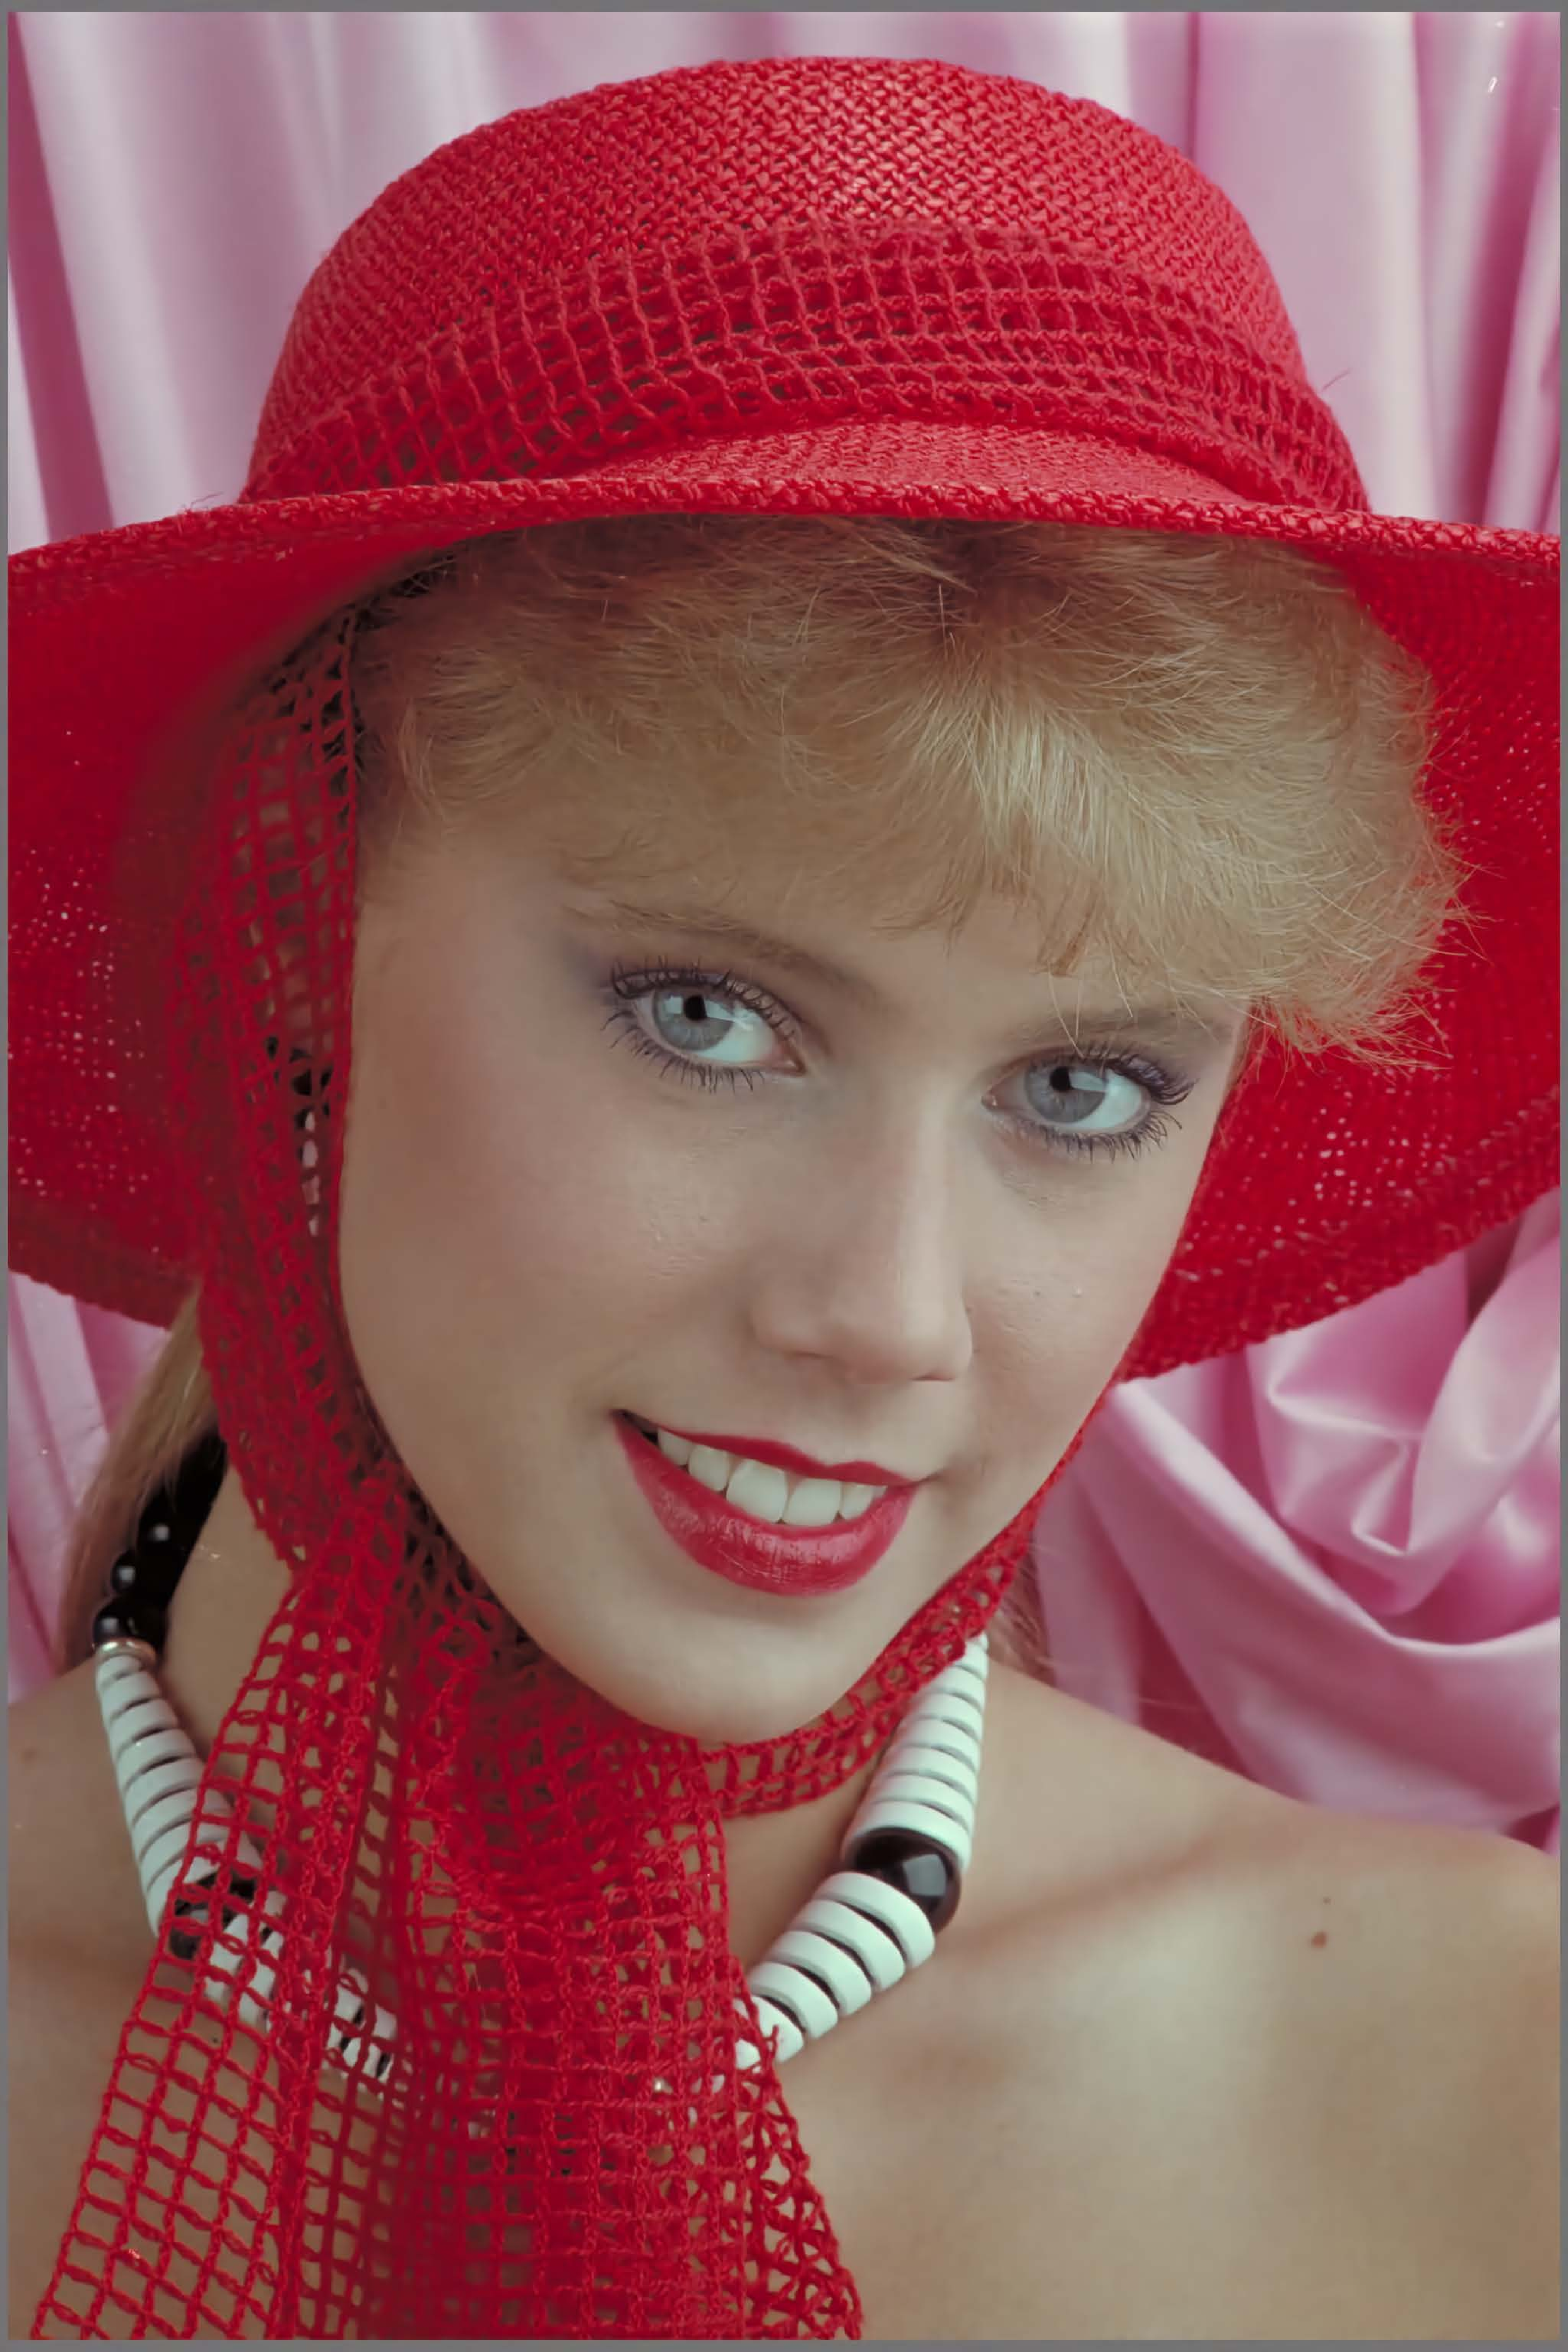
\includegraphics[width=\textwidth]{Immagini/IMAGES/mbt2018_mean_3_IMG0004.pdf}
        \caption{mbt2018 mean}
        \label{fig:CompressedMbt2018Mean}
    \end{subfigure}
    \caption{Confronto PNG con Ballè2018 a 0.145 bpp}
    \label{fig:CompressionMbt2018}
\end{figure}

\begin{figure}[t!]
    \centering
    \begin{subfigure}[]{0.25\textwidth}
        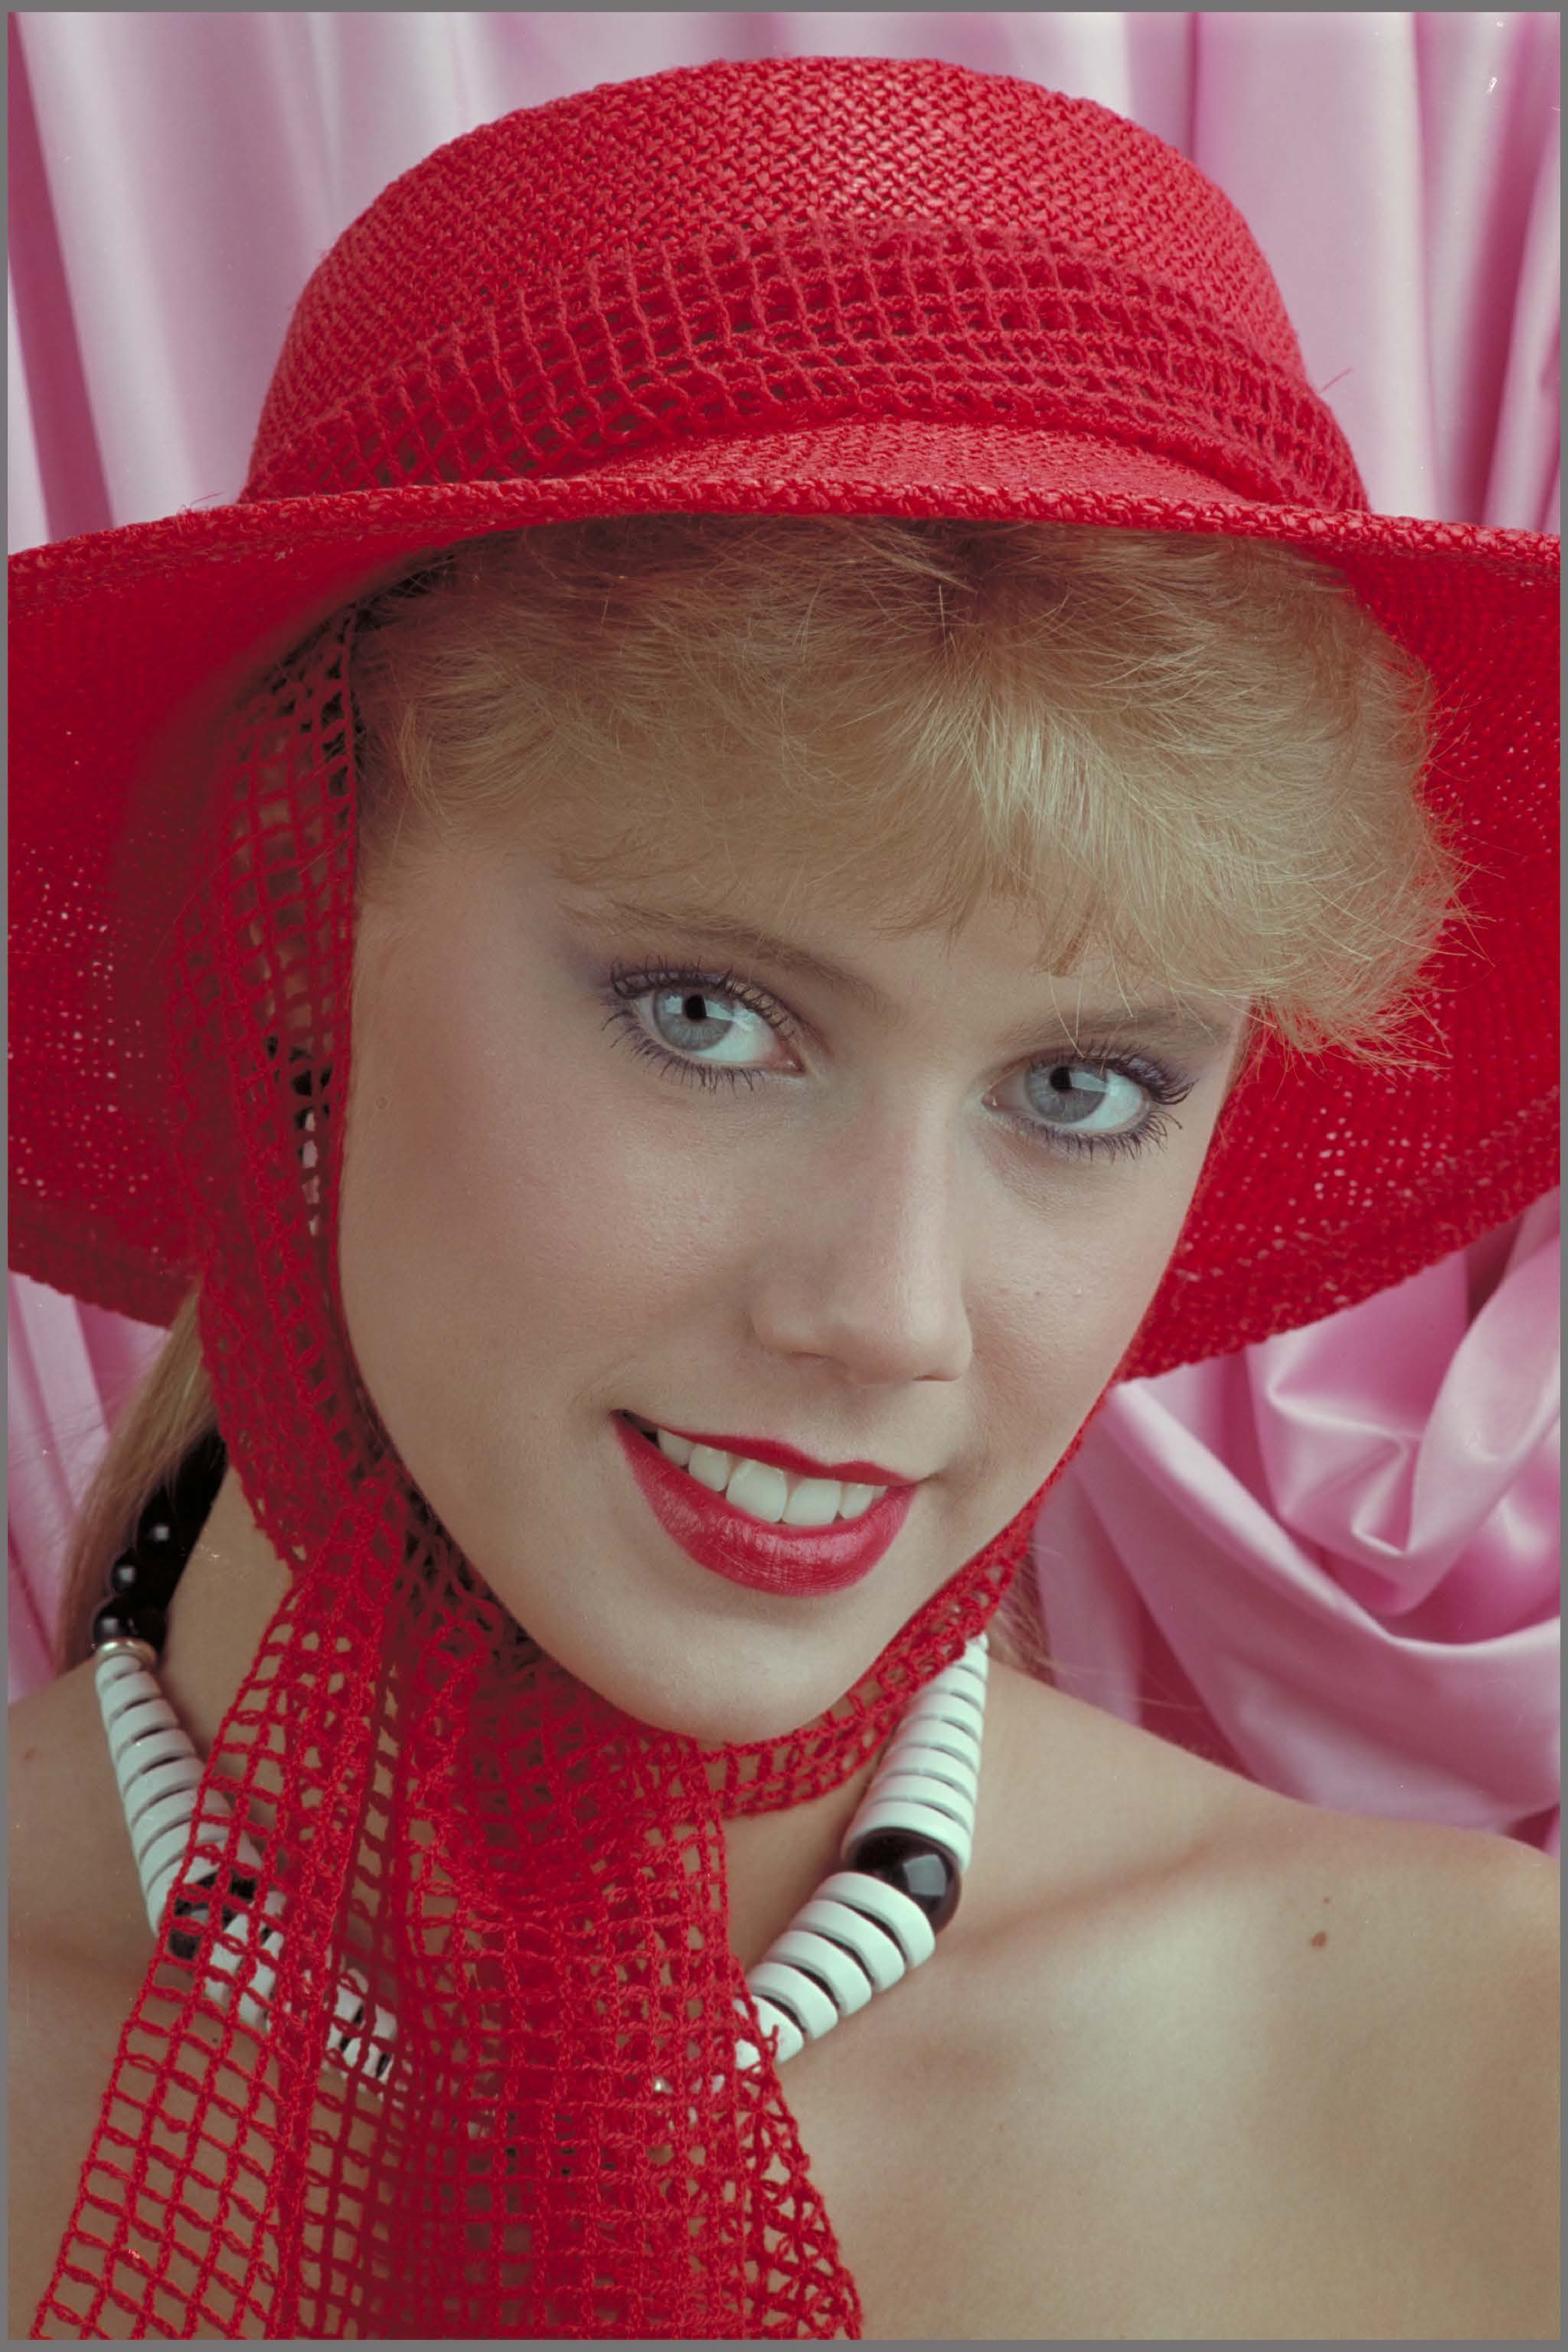
\includegraphics[width=\textwidth]{Immagini/IMAGES/PNG_IMG0004.pdf}
        \caption{Originale}
        \label{fig:OriginalChang2020}
    \end{subfigure}
    \hspace*{0.5cm}
    \begin{subfigure}[]{0.25\textwidth}
        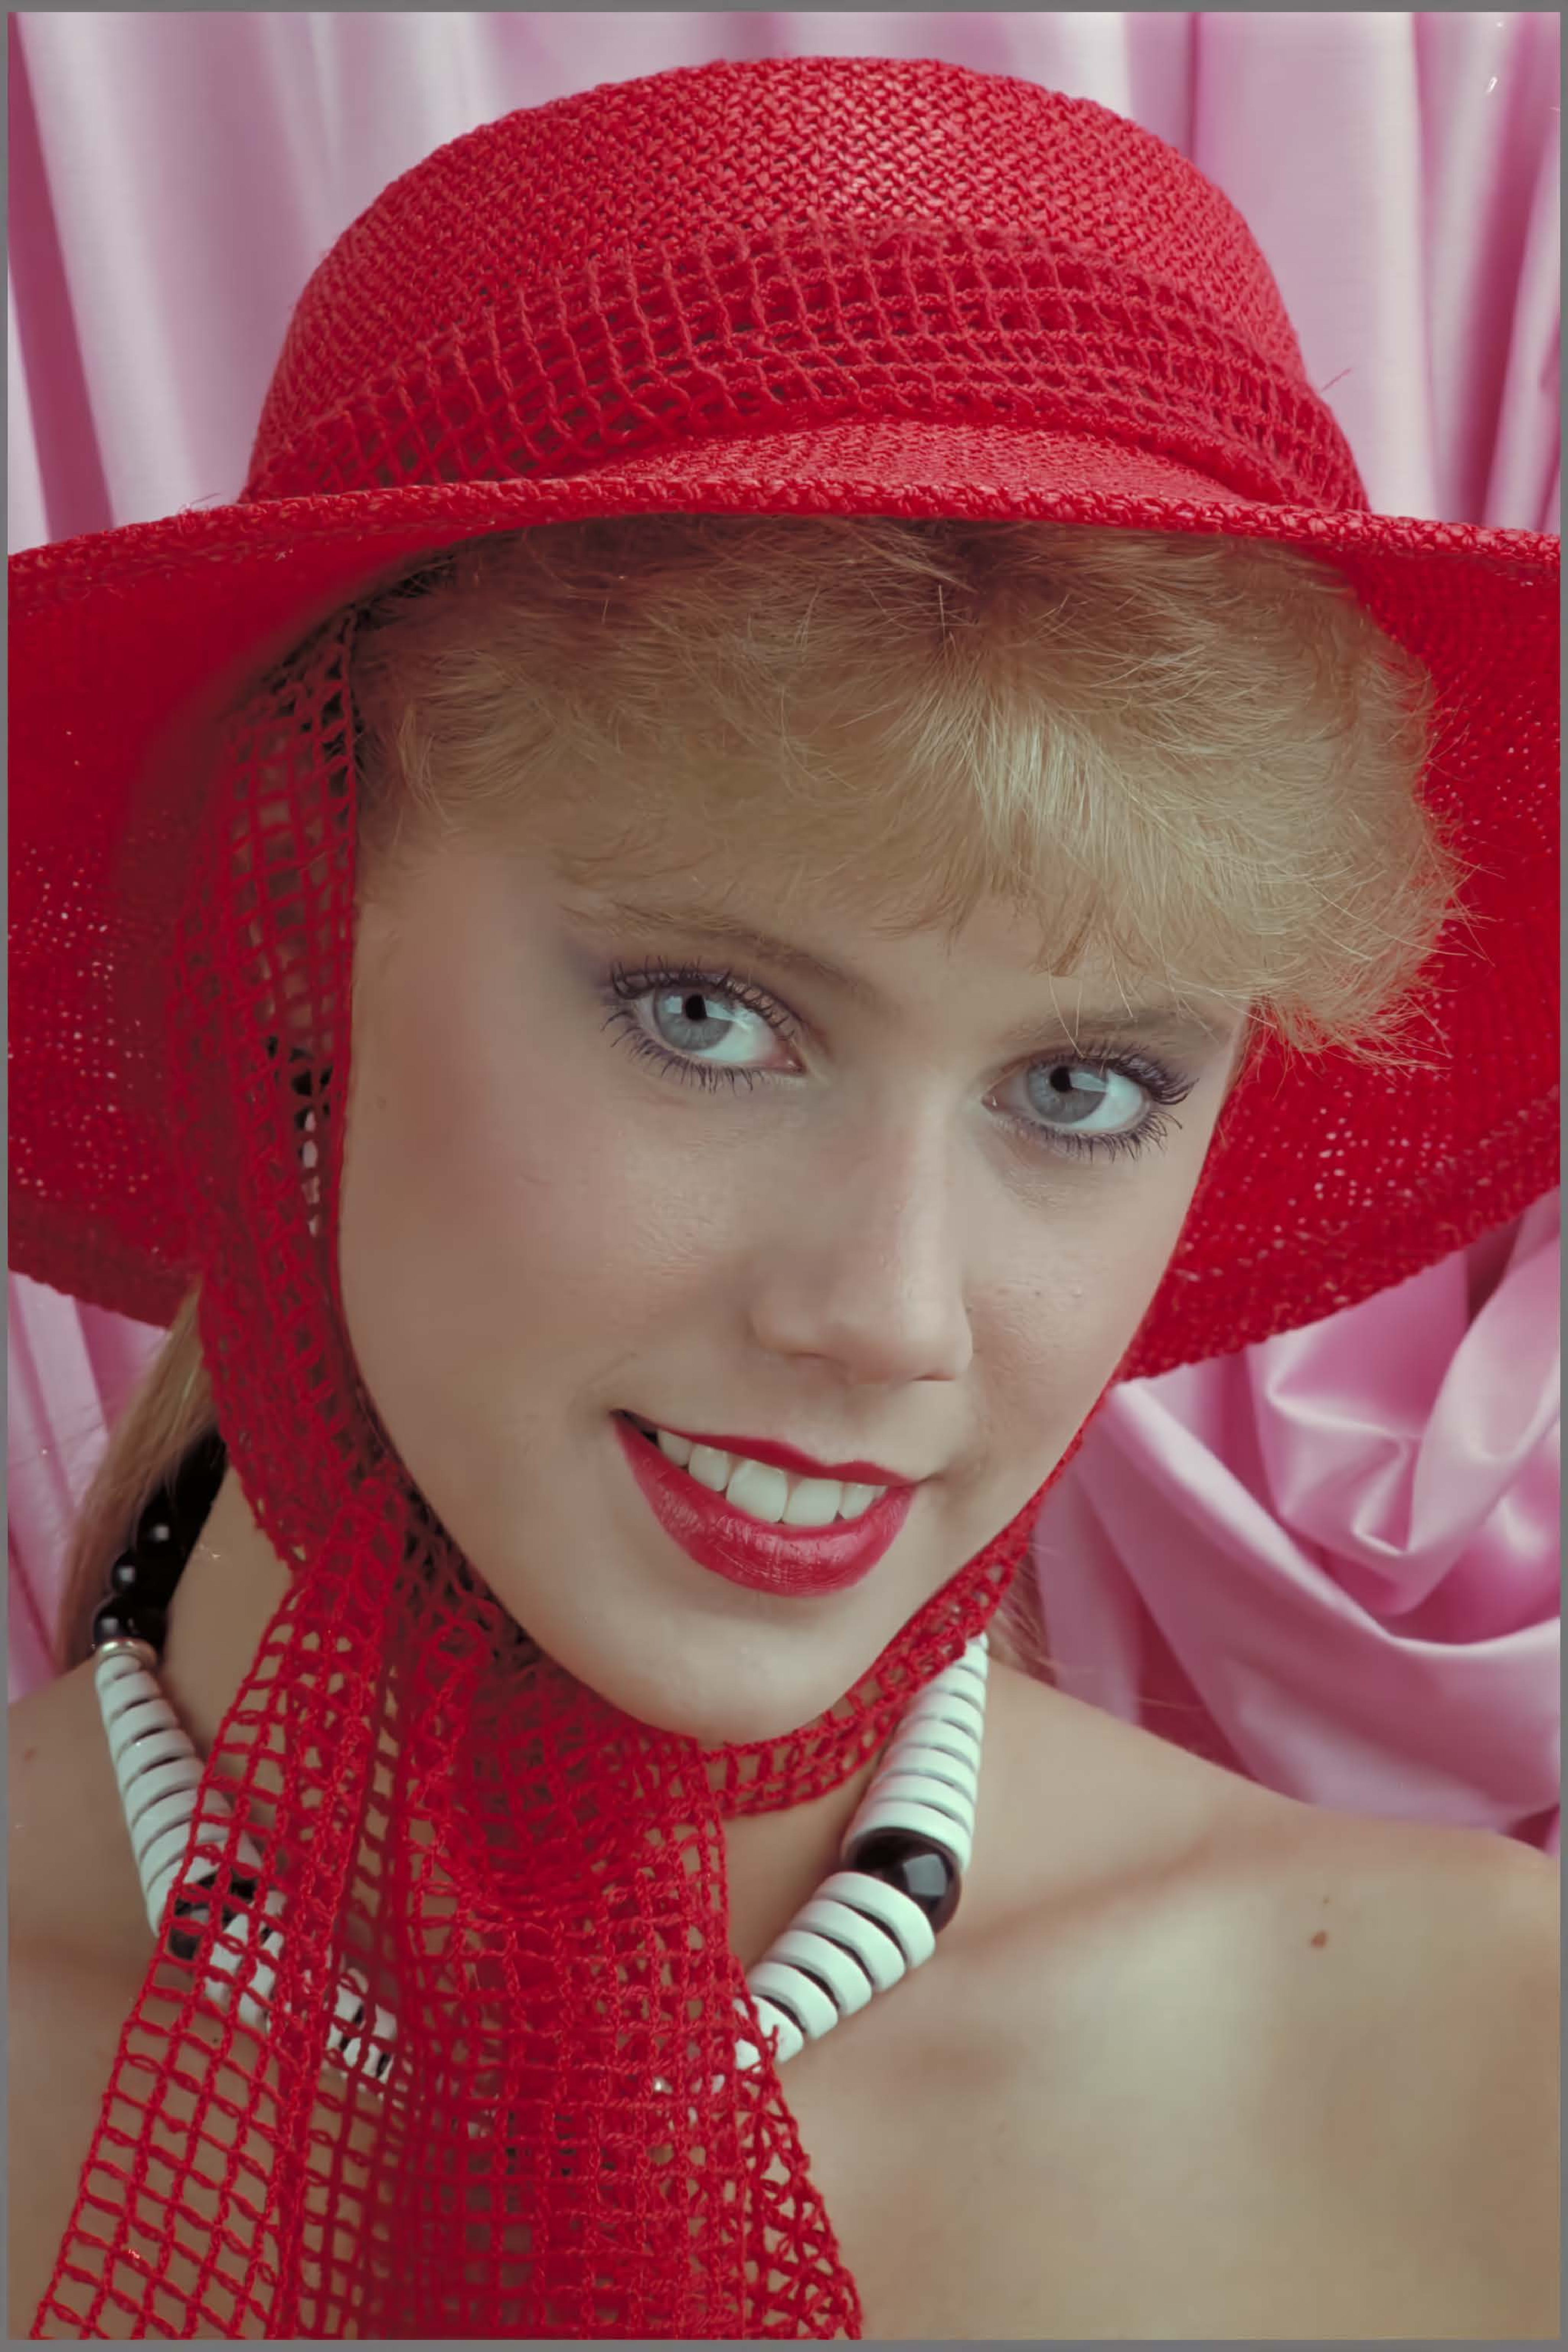
\includegraphics[width=\textwidth]{Immagini/IMAGES/cheng2020_attn_3_IMG0004.pdf}
        \caption{Cheng2020}
        \label{fig:CompressedCheng2020}
    \end{subfigure}
    \hspace*{0.5cm}
    \begin{subfigure}[]{0.25\textwidth}
        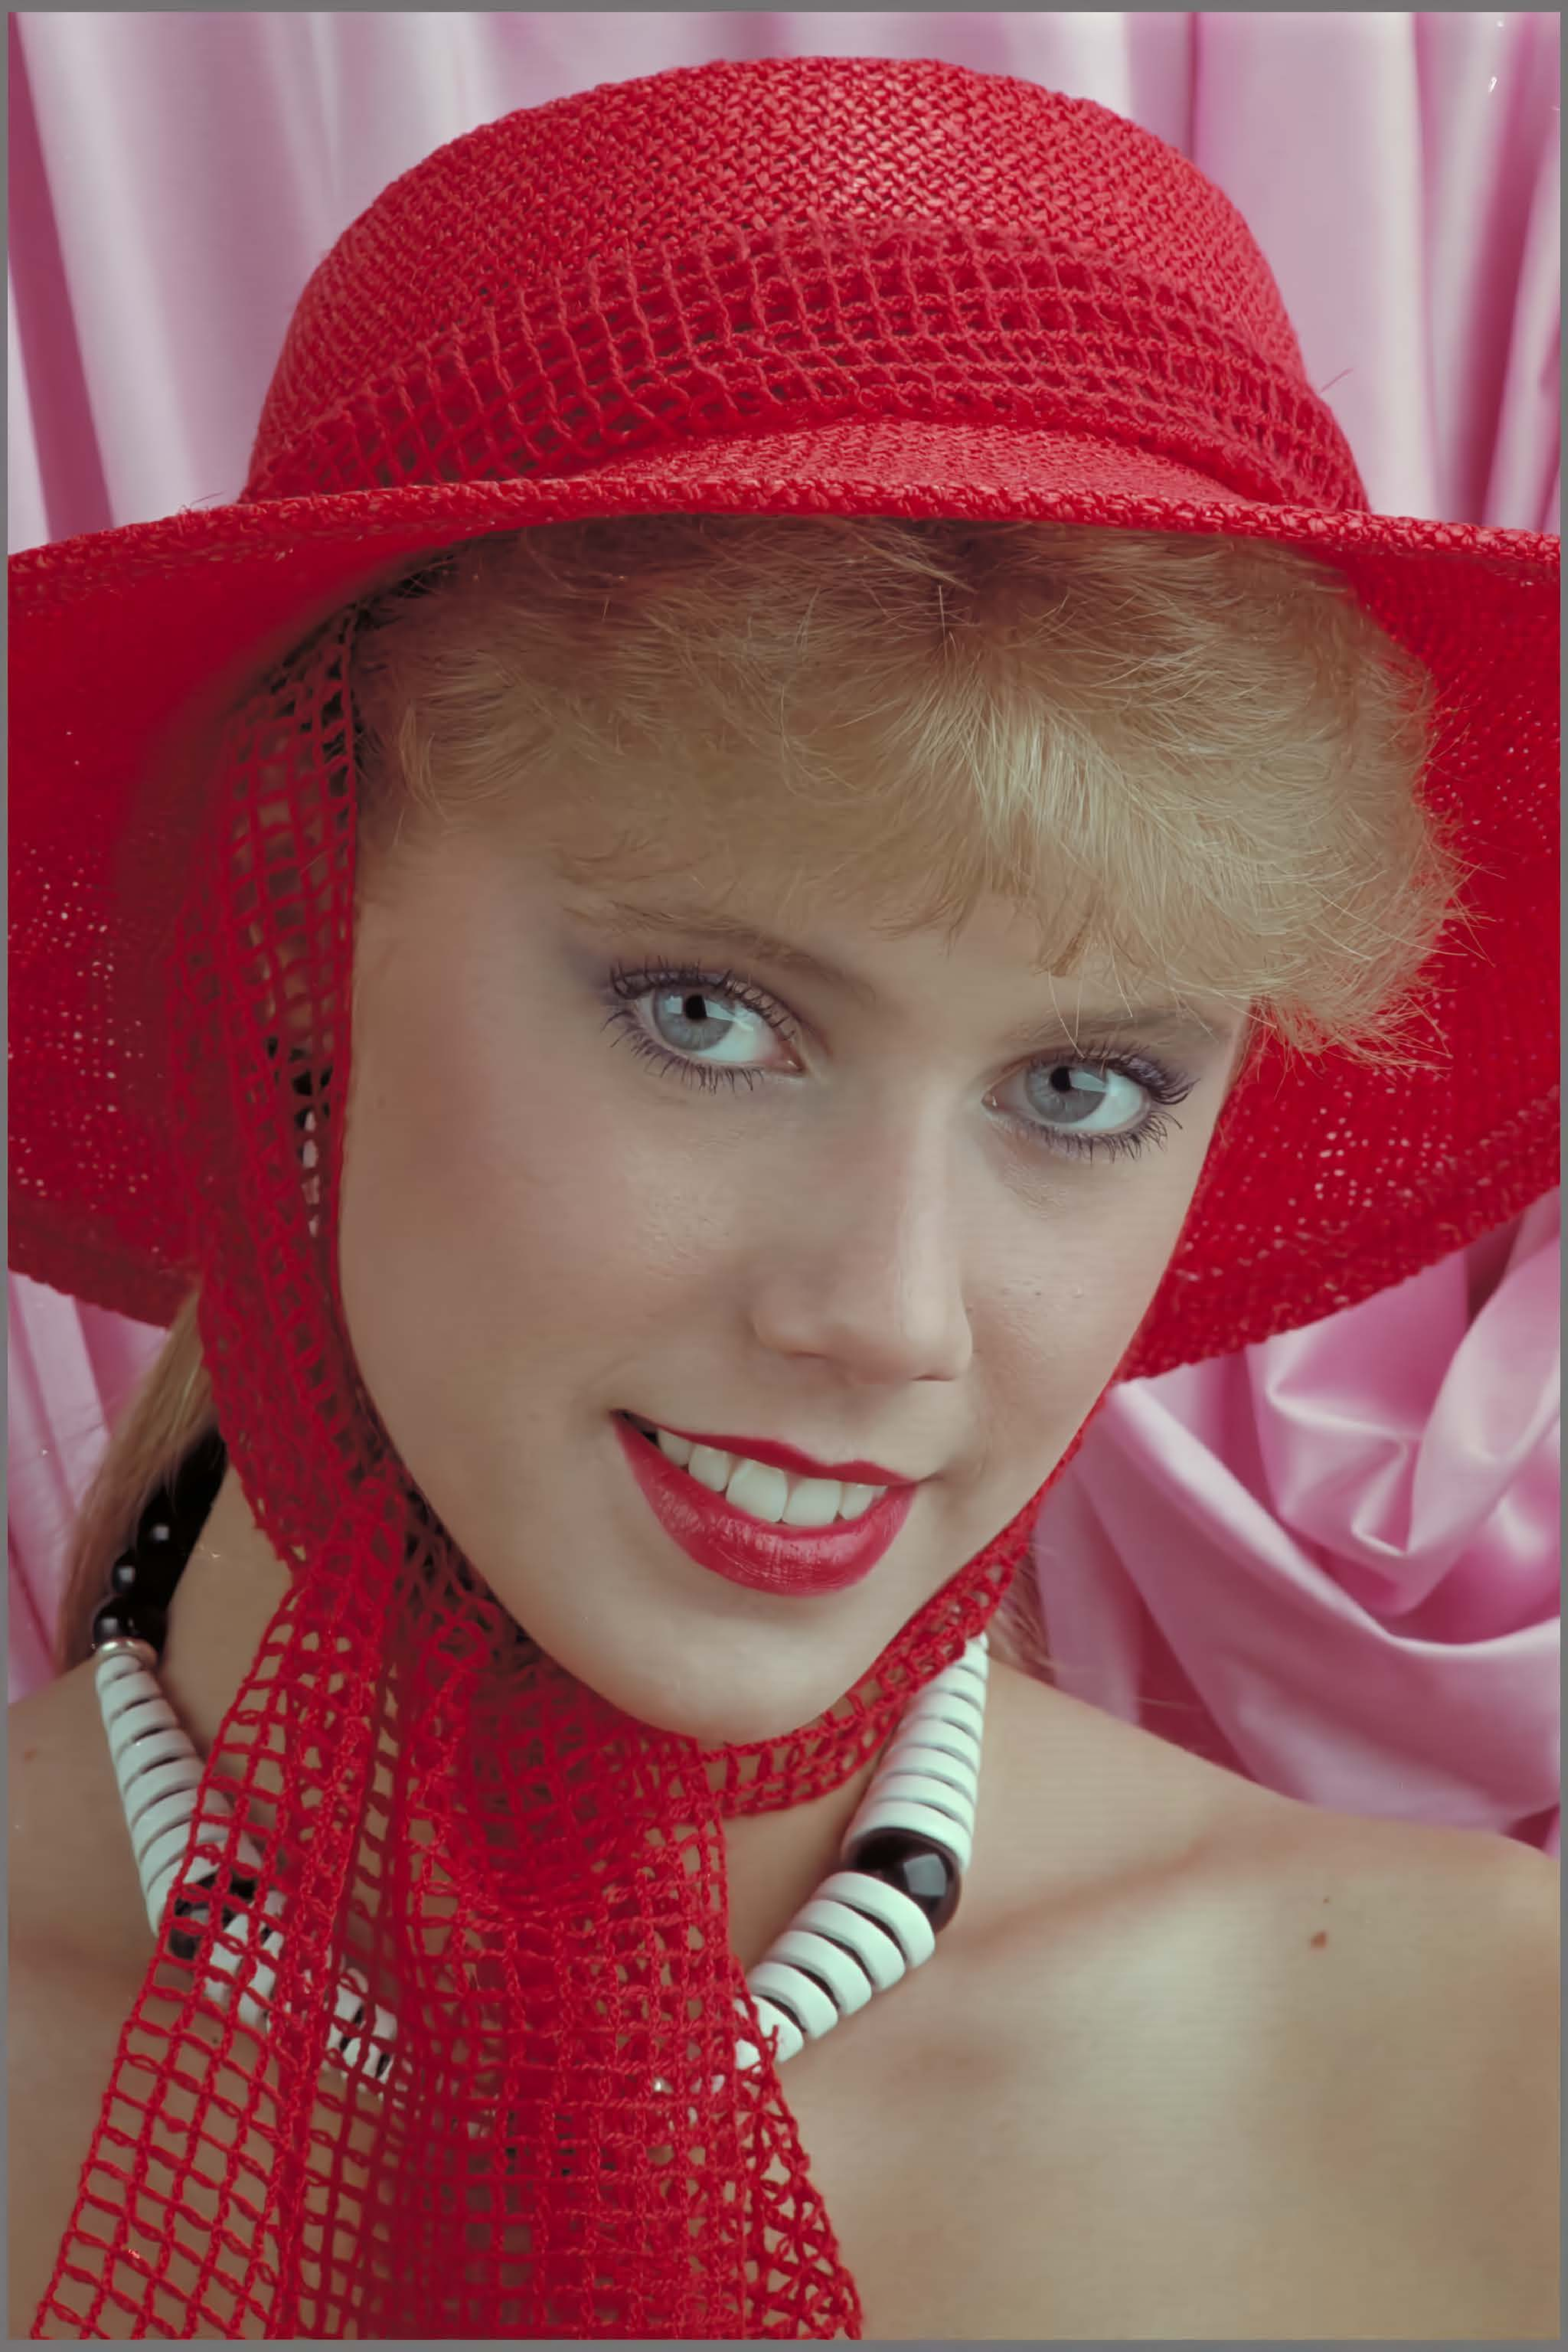
\includegraphics[width=\textwidth]{Immagini/IMAGES/cheng2020-anchor_3_IMG0004.pdf}
        \caption{Cheng2020 attention}
        \label{fig:CompressedCheng2020Attention}
    \end{subfigure}
    \caption{Confronto PNG con Cheng2020 a 0.123 bpp}
    \label{fig:CompressionCheng2020}
\end{figure}
    \chapter{Valutazione delle prestazioni}
In questo capitolo vogliamo comparare gli algoritmi tradizionali descritti nel capitolo 1 con due degli algoritmi descritti nel capitolo 2, nello specifico Ballè et al. \cite{minnen2018joint} e Cheng et al. \cite{cheng2020learned}. Purtroppo non siamo stati in grado di testare anche Wang et al. \cite{wang2022neural} in quanto, nonostante abbiano reso il modello disponibile, non ne hanno fornito una versione pre addestrata.\\
L’hardware su cui sono stati eseguiti i test è un computer dotato di processore AMD Ryzen 5 5600X con 6 core e 12 thread a 3.7GHz, munito di 16GB di ram DDR4 a 3200MHz e come sistema operativo una distribuzione Fedora Linux 38 con kernel linux 6.5.7-200. Vogliamo sottolineare anche che per realizzare delle misurazioni più vicine alla realtà possibili abbiamo deciso di non utilizzare GPU, in quanto non tutti i computer sono dotati di GPU su cui è possibile eseguire Tensorflow o PyTorch e non abbiamo preso particolari precauzioni per garantire l’esecuzione esclusiva del codice, abbiamo lasciato che il codice concorresse con il sistema operativo e le applicazioni in background per l’allocazione del processore, tutto per simulare un ambiente più simile ad un caso reale.\\
Per effettuare i vari test sono stati realizzati dei notebook in python 3.11 su jupyterlab 4.0.7. I codificatori che abbiamo utilizzato sono i seguenti. Per comprimere le immagini con JPEG abbiamo utilizzato Pillow 10.0.1 \cite{PillowLibrary} sviluppato da Jeffrey A. Clark. Per comprimere le immagini con JPEG2000 abbiamo utilizzato OpenJPEG 2.5.0 \cite{OpenJPEGLibrary} sviluppato dall’ Université de Louvain. Per comprimere con BPG abbiamo usato il framework messo a disposizione da F.Bellard \cite{BPGImageformat} nella versione 0.9.8. Per comprimere con VVC abbiamo usato il framework distribuito da Fraunhofer HHI \cite{VVCLibrary} che comprende l’encoder vvencapp 1.9.1 e il decocder vvdecapp 2.1.2. Per comprimere con le due reti abbiamo utilizzato la libreria compressai 1.2.4 \cite{CompressAILibrary} in cui sono presenti le implementazioni pre allenate dei due modelli che ci interessano. Dei due modelli sono presenti due versioni, per Ballé et al. \cite{minnen2018joint} è fornita un implementazione in cui la media della distribuzione gaussiana viene bloccata a 0 e una in cui la media è un parametro determinato durante la compressione, per Cheng at al. 2020 \cite{cheng2020learned} viene fornita una versione che fa uso degli attention module e una in cui sono disabilitati.\\
Per valutare i vari metodi abbiamo utilizzato 24 immagini non compresse di dimensione $2048\:x\:3072$ con spazio di colore RGB a 8 bit per canale, prese dal database di Kodak \cite{KodakDataset}. I vari algoritmi sono stati eseguiti più volte con vari livelli di qualità, che andremo ad approfondire successivamente, ed infine sono state calcolate le metriche sui risultati ottenuti.\\

\section{Metriche utlizzate}
Per valutare le prestazioni facciamo affidamento ad alcune metriche che ci permettono di confrontare le varie tecniche. Molte di queste metriche sono oggettive, alcune invece cercano di quantificare il più fedelmente possibile quella che è la qualità percepita da un osservatore umano.
Passiamo ora ad introdurre brevemente le metriche e come vengono calcolate.\\

\subsection{BPP}
Per valutare quanto un’immagine sia stata compressa utilizziamo il numero di bit necessari per rappresentare un pixel dell’immagine $x$, o bit per pixel. Il calcolo \ref{eq:bpp} di questo parametro è molto semplice ed intuitivo.\\
\begin{equation}\label{eq:bpp}
    bpp(x) = \dfrac{taglia (x)}{larghezza (x) \cdot altezza (x)}
\end{equation}\\
Dove con taglia indichiamo il numero di bit occupati dall’immagine compressa, con larghezza intendiamo il numero di pixel in una riga orizzontale dell’immagine e con altezza intendiamo il numero di pixel in una riga verticale dell’immagine.\\
Lo spezzone di codice \ref{code:bppComputation} mostra come è stato calcolata la metrica bit per pixel.\\
\begin{adjustbox}{max width=\textwidth}
    \begin{lstlisting}[language=Python, caption=Spezzone di codice per il calcolo dei bit per pixel, label=code:bppComputation]
        from PIL import Image
        import os
        
        image = Image.open(file)
        file_size = os.path.getsize(file) * 8
        pixels = image.width * image.height
        bits_per_pixel = file_size/pixels
    \end{lstlisting}
\end{adjustbox}

\subsection{Tempo di codifica}
Per valutare la velocità con la quale un algoritmo di codifica riesce a produrre la rappresentazione compressa di un’immagine andiamo a misurare il tempo che intercorre tra la chiamata al codificatore e il termine dell’esecuzione del processo di codifica. Avendo utilizzato python per richiamare i codificatori abbiamo usato il modulo timeit di per calcolare i tempi di esecuzione.\\
Lo spezzone di codice \ref{code:CompressionTime} mostra come è stata usata la libreria per calcolare i tempi di esecuzione.\\
\begin{adjustbox}{max width=\textwidth}
    \begin{lstlisting}[language=Python, caption=Spezzone di codice per il calcolo del tempo di compressione, label=code:CompressionTime]
        import timeit
        
        starttime = timeit.default_timer()
        call_to_encoder() #Chiamata encoder
        endtime = timeit.default_timer()
        execution_time = endtime-starttime #Caloclo del tempo in secondi
    \end{lstlisting}
\end{adjustbox}

    
\subsection{PSNR}
L’ultima delle metriche oggettive che andiamo a considerare è il Peak Signal to Noise Ratio o PSNR. Questa metrica, espressa in scala logaritmica, rappresenta il rapporto tra la potenza del segnale originale e la potenza del rumore introdotto dal processo di compressione, dunque più alto è il valore del PSNR più l’immagine compressa è fedele all’originale.\\
Per poter calcolare il PSNR occore definire cosa sia e come si calcola l’MSE per immagini a colori, ovvero con più componenti.\\
L’ Errore Quadratico Medio o MSE indica la distanza al quadrato tra il valore di un pixel dell’immagine e il valore dello stesso pixel nell’immagine distorta. Per calcolare l’MSE di una singola componente di colore si utilizza la formula \ref{eq:MSE}, dove $M$ ed $N$ indicano rispettivamente la larghezza e l'altezza in pixel delle immagini orginale $R$ e compressa $C$.\\
\begin{equation}\label{eq:MSE}
    MSE(R,C) = \dfrac{1}{MN} \sum_{i=0}^{M-1} \sum_{j=0}^{N-1} || R(i,j) - C(i,j) ||^{2}
\end{equation}\\
Nel caso di immagini a colori però non abbiamo una sola componente ma ne abbiamo al minimo due, bisogna dunque definire come combinare gli MSE delle singole componenti, in base allo spazio di colore scelto, in un’unica metrica globale per l’immagine.\\
Nel nostro caso, avendo scelto lo spazio di colore YUV, la combinazione degli MSE delle singole componenti si ottiene con la formula \ref{eq:wMSE}, nella quale possiamo osservare che l’MSE globale dell’immagine non è altro che la somma pesata degli MSE delle singole componenti.\\
Questi pesi sono utilizzati per attribuire più importanza al canale $Y$, in quanto le informazioni in questo canale sono quelle maggiormente responsabili della qualità dell’immagine.\\
\begin{equation}\label{eq:wMSE}
    MSE(R,C) = (\dfrac{3}{4}) \cdot MSE_{Y}(R,C) + (\dfrac{1}{8}) \cdot MSE_{U}(R,C)  +  (\dfrac{1}{8}) \cdot MSE_{V}(R,C)
\end{equation}\\
Avendo definito come si calcola l’MSE pesato, il calcolo del PSNR pesato si ottiene con la formula \ref{eq:PSNR}, in cui $I$ indica il massimo valore che il pixel di un canale può assumere, nel nostro caso essendo i canali nello spazio di colore YUV rappresentati con 8 bit ciascuno, il valore di $I$ è 255.\\
\begin{equation}\label{eq:PSNR}
    PSNR(R,C)  =  10 * \log{\dfrac{I^2}{MSE(R,C)}}_{10}
\end{equation}\\
Questa metrica è uno standard nella comunità scientifica per l’analisi della qualità dei sistemi che operano con immagini, solitamente viene calcolata per immagini con gli spazio di colore YUV o YCbCr.\\
Per il calcolo abbiamo usato la libreria scikit-image 0.22.0 per calcolare l’MSE dei singoli canali per poi combinarli e calcolare il PSNR, come possiamo vedere nello spezzone di codice \ref{code:PSNRComputation}.\\
\begin{adjustbox}{max width=\textwidth}
    \begin{lstlisting}[language=Python, caption=Spezzone di codice per il calcolo del PSNR pesato, label=code:PSNRComputation]
        from skimage import metrics
        
        YMSE = metrics.mean_squared_error(OY,Y)
        UMSE = metrics.mean_squared_error(OU,U)
        VMSE = metrics.mean_squared_error(OV,V)
        MSE = (3/4)*YMSE + (1/8)*UMSE + (1/8)*VMSE
        psnr = 10 * numpy.log10((255*255) / MSE)
        print(‘PSNR: ’+str(msssim)+’dB’)
    \end{lstlisting}
\end{adjustbox}   
    

\subsection{MSSIM}
La prima metrica che cerca di fornire un indice di qualità percepita che andremo a considerare è il MultiScale Structural Similarity for IMage quality assessment o MS-SSIM. \cite{wang2003multiscale}.\\
Lo sviluppo di questo indice si basa sull’assunto che il sistema visivo umano è altamente adatto per estrarre informazioni strutturali dalle immagini, dunque una misura di similarità strutturale dovrebbe fornire una buona approssimazione della qualità percepita da un osservatore umano.\\
Per il calcolo dell’MS-SSIM, come possiamo vedere nell’equazione \ref{eq:ms-ssim}, si deve eseguire il prodotto pesato di tre indici, un indice di luminanza $l$, un indice di contrasto $c$ e un indice di struttura $s$, per la stessa immagine scalata $M$ volte. Questi indici sono pesati da tre esponenti, rispettivamente $\alpha_{M}\:\beta_{j}\:\gamma_{j}$, e come possiamo osservare solamente due dei componenti vengono pesati per ogni scalatura dell’immagine, la luminanza invece viene calcolata solo per l’indice di qualità $M$.\\
\begin{equation}\label{eq:ms-ssim}
    MS-SSIM(R,C) = [l_{M}(R,C)]^{\alpha_{M}} \cdot \prod_{j=1}^{M}[c_{j}(R,C)]^{\beta_{j}} [s_{j}(R,C)]^{\gamma_{j}} 
\end{equation}\\
L’indice $M$ rappresenta la scalatura delle immagini in ingresso, se l’indice è uguale a 1 ci stiamo riferendo esattamente alle immagini da valutare. Ad ogni incremento di $M$ all’immagine originale viene applicato un filtro passa basso e viene sotto campionata di un fattore 2. Dopo esattamente $M-1$ iterazioni l’immagine non sarà più riducibile e la computazione termina.\\
Questa è la seconda metrica standard che viene utilizzata dalla comunità scientifica per valutare le prestazioni di algoritmi che operano su immagini, in quanto a differenza del PSNR, questa rappresenta un giudizio più soggettivo.\\
Per il calcolo dell’MS-SSIM abbiamo usato la libreria pytorch-msssim 1.0.0 che fornisce una semplice funzione per il calcolo di questa metrica, l’unica accortezza da dover prendere è quella di convertire le immagini da valutare in tensori normalizzati prima di passare le immagini alla funzione, come possiamo vedere nello spezzone di codice \ref{code:MSSSIMComputation}.\\
\begin{adjustbox}{max width=\textwidth}   
    \begin{lstlisting}[language=Python, caption=Spezzone di codice per il calcolo dell'MS-SSIM, label=code:MSSSIMComputation]
        import torch
        from skimage import metrics
        from torchvision import transforms
        
        device = 'cuda' if torch.cuda.is_available() else 'cpu'
        
        reference = transforms.ToTensor()(reference_image).unsqueeze(0).to(device)
        compressed = transforms.ToTensor()(compressed_image).unsqueeze(0).to(device)
        msssim = ms_ssim(reference, compressed, data_range=1, size_average=True)
        print(‘MS-SSIM: ’+str(msssim))
    \end{lstlisting}
\end{adjustbox} 


\subsection{LPIPS}
L’ultima metrica che andremo ad utilizzare è anch'essa soggettiva e utilizza delle reti neurali per valutare la distanza percepita tra l’immagine originale e l’immagine compressa, la tecnica proposta da Zhang et al. nel 2018 \cite{zhang2018unreasonable} prende il nome di Learned Perceptual Image Patch Similarity o LPIPS.\\
L’osservazione su cui si basa lo sviluppo di questa metrica è il fatto che l’attivazione interna dei neuroni di reti utilizzata per compiti di classificazione di immagini ad alto livello possono essere utilizzate per calcolare una distanza percepita tra due immagini. Durante lo sviluppo di questa metrica il team di Zhang et al. ha scoperto non solo che questa si rivela essere un’ottima metrica, ma riesce anche ad emulare molto bene i giudizi dati da degli osservatori umani, la maggior parte delle volte anche in modo migliore rispetto ad altre metriche più affermate, come il precedentemente citato MS-SSIM.\\
Le reti che sono state valutate dal team di Zhang et al. sono SqueezeNet, AlexNet e VGG, a queste reti vengono fornite le due immagini $x$ e $x_{0}$, rispettivamente originale e distorta. Dalle reti vengono poi estratte le feature da $L$ livelli, rispettivamente $\hat{y}^l$ e $\hat{y}_{0}^l$ e vengono normalizzate rispetto alla dimensione dei canali. Le attivazioni dei vari canali vengono poi pesate con un vettore di pesi $w^l$ e ne viene calcolata la distanza $L_{2}$, come possiamo vedere nell’equazione \ref{eq:LPIPSExtraction}.\\
\begin{equation}\label{eq:LPIPSExtraction}
    d(x,x_{0}) = \sum_{l}\dfrac{1}{H_{l}W_{l}} \sum_{h,w} || w_{l} \cdot (\hat{y}_{hw}^{l} - \hat{y}_{0,hw}^{l}) ||_{2}^{2}
\end{equation}\\
Noi abbiamo scelto di utilizzare la metrica LPIPS con rete AlexNet, in quanto dai risultati sperimentali, nonostante non sia la tecnica più avanzata, fornisce la valutazione più simile a quella data da degli osservatori umani.\\
Il team di Zhang et al. fornisce anche una libreria per python che abbiamo utilizzato per i nostri test nella versione 0.1.4, nello spezzone di codice \ref{code:LPIPSComputation} mostriamo l'uso di tale libreria.\\
\begin{adjustbox}{max width=\textwidth}   
    \begin{lstlisting}[language=Python, caption=Spezzone di codice per il calcolo di LPIPS con AlexNet, label=code:LPIPSComputation]
        import torch
        from torchvision import transforms
        import lpips
        
        loss_fn_alex = lpips.LPIPS(net='alex')
        
        reference = transforms.ToTensor()(reference_image).unsqueeze(0).to(device)
        compressed = transforms.ToTensor()(compressed_image).unsqueeze(0).to(device)
        d = loss_fn_alex(transforms.Normalize(mean=(0.5, 0.5, 0.5),
                         std=(0.5, 0.5, 0.5))(reference),transforms.Normalize(mean=(0.5, 0.5, 0.5),
                         std=(0.5, 0.5, 0.5))(compressed))[0].item()
        print(‘LPIPS: ’+str(d))
    \end{lstlisting}
\end{adjustbox} 
    

\section{Presentazione dei risultati}
Andiamo ora a presentare i risultati sperimentali ottenuti dalla compressione delle immagini del dataset Kodak con gli algoritmi precedentemente descritti. Per ogni metodo di compressione vengono analizzati cinque diversi livelli di qualità comparati con le metriche appena descritte. I livelli vengono scelti andando ad agire sui parametri di qualità degli encoder, per cercare di mantenere il confronto equo abbiamo cercato di ottenere circa gli stessi livelli per ogni metodo di compressione. Tutte i valori che andremo a presentare sono le medie delle metriche sulle 24 immagini del dataset.\\
Il primo livello significativo si trova in corrispondenza di $0.16bpp$, i tempi di compressione per questo livello di qualità sono visibili nell’immagine \ref{fig:times16}. Il secondo livello si trova in corrispondenza di $0.21bpp$, dei cui tempi di compressione sono riportati nell’immagine \ref{fig:times21}. Il terzo livello che andiamo a considerare si ha per $0.34bpp$, i tempi di compressione per questo livello sono riportati nel grafico\ref{fig:times34}.\\
Un ulteriore livello di qualità si ha in corrispondenza di $0.07bpp$, JPEG non riesce però a comprimere fino a questi livelli, mentre la misurazione di JPEG2000 non è stata fatta perché si è preferito prendere una misura per un livello di qualità più elevato. I tempi di compressione per questo livello sono stati comunque calcolati in quanto è interessante osservare il comportamento del codec VVC, e sono riportati nell’immagine \ref{fig:times07}.\\
L’ultimo livello di qualità invece si ha per $0.41bpp$ dove però non abbiamo le misurazioni delle reti, in quanto non sono presenti i modelli pre addestrati per queste qualità. I tempi di compressione per quest’ultimo livello sono visibili nella figura \ref{fig:times41}.\\

\begin{figure}[!h]
    \centering
    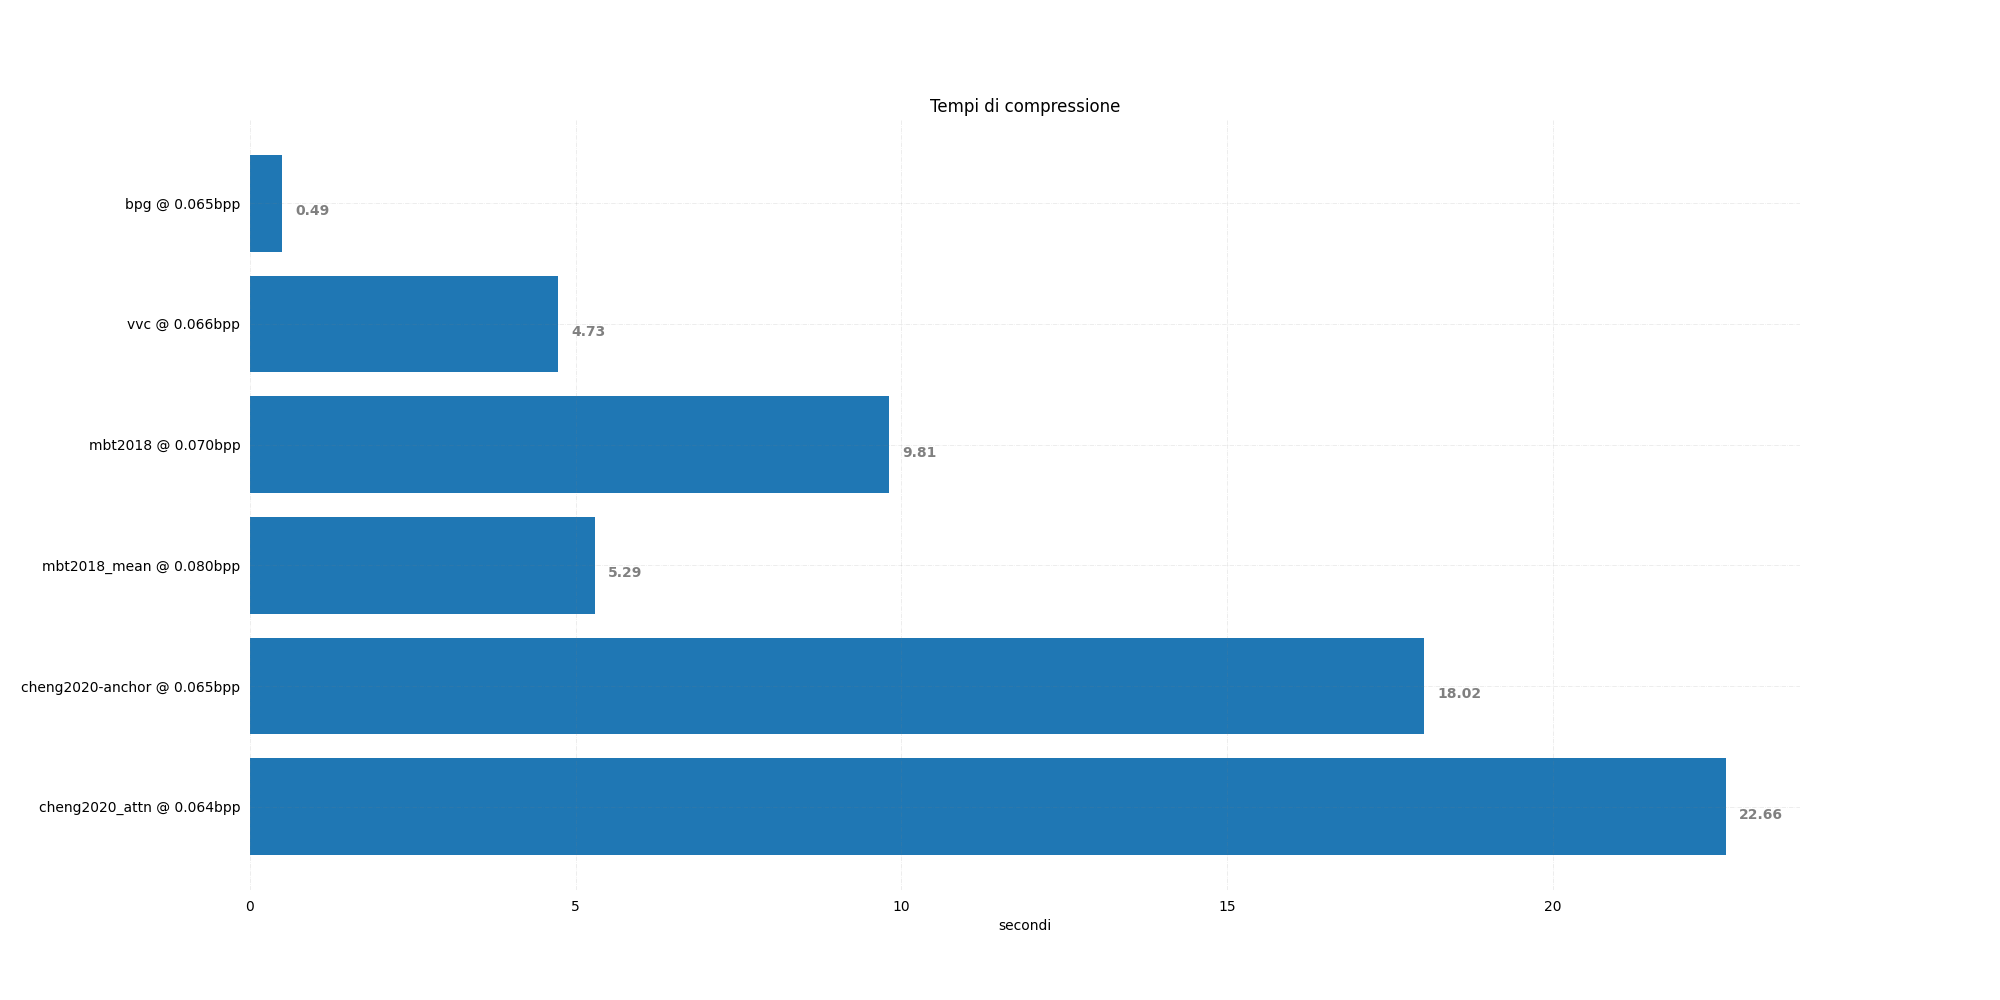
\includegraphics[width=1\textwidth]{Immagini/METRICS/times@0.07bpp.png}
    \caption{Tempi di compressione a 0.07 bpp}
    \label{fig:times07}
\end{figure}
\newpage
\begin{figure}[!h]
    \centering
    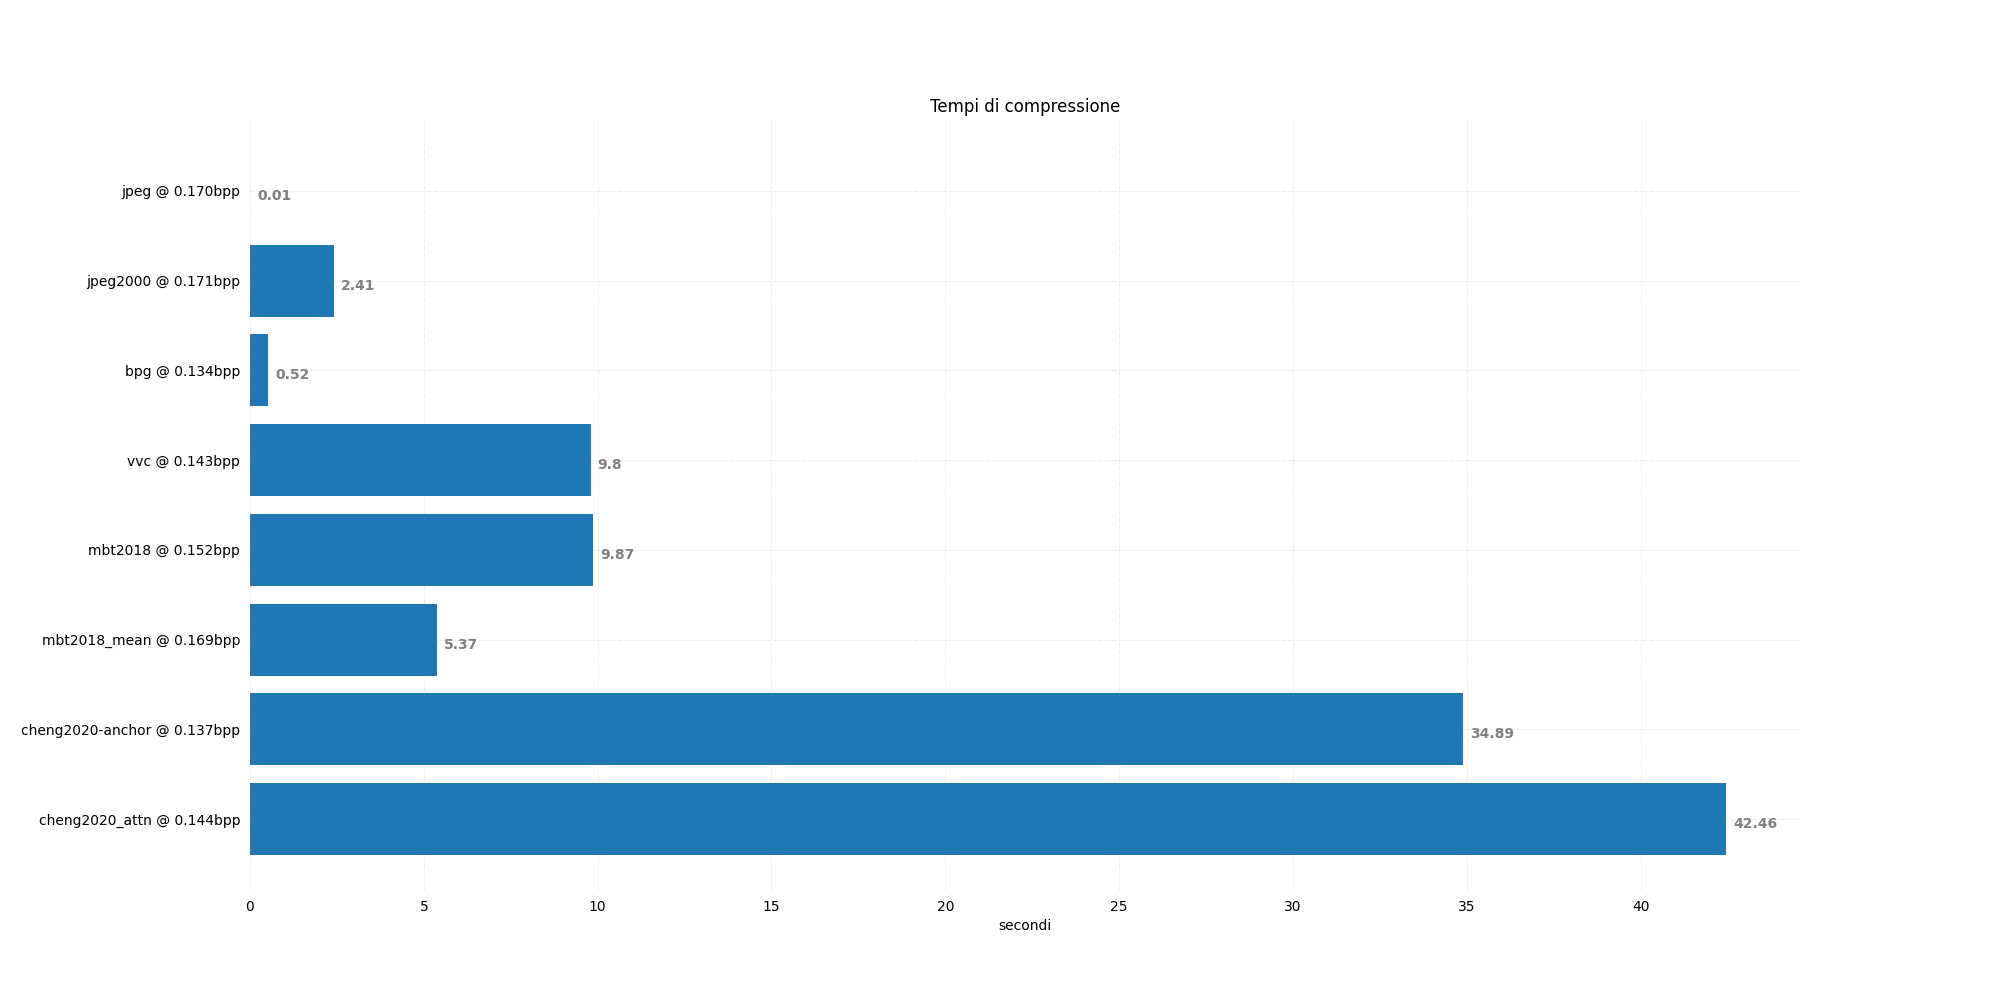
\includegraphics[width=1\textwidth]{Immagini/METRICS/times@0.16bpp.png}
    \caption{Tempi di compressione a 0.16 bpp}
    \label{fig:times16}
\end{figure}
\hspace{0.5cm}
\begin{figure}[!h]
    \centering
    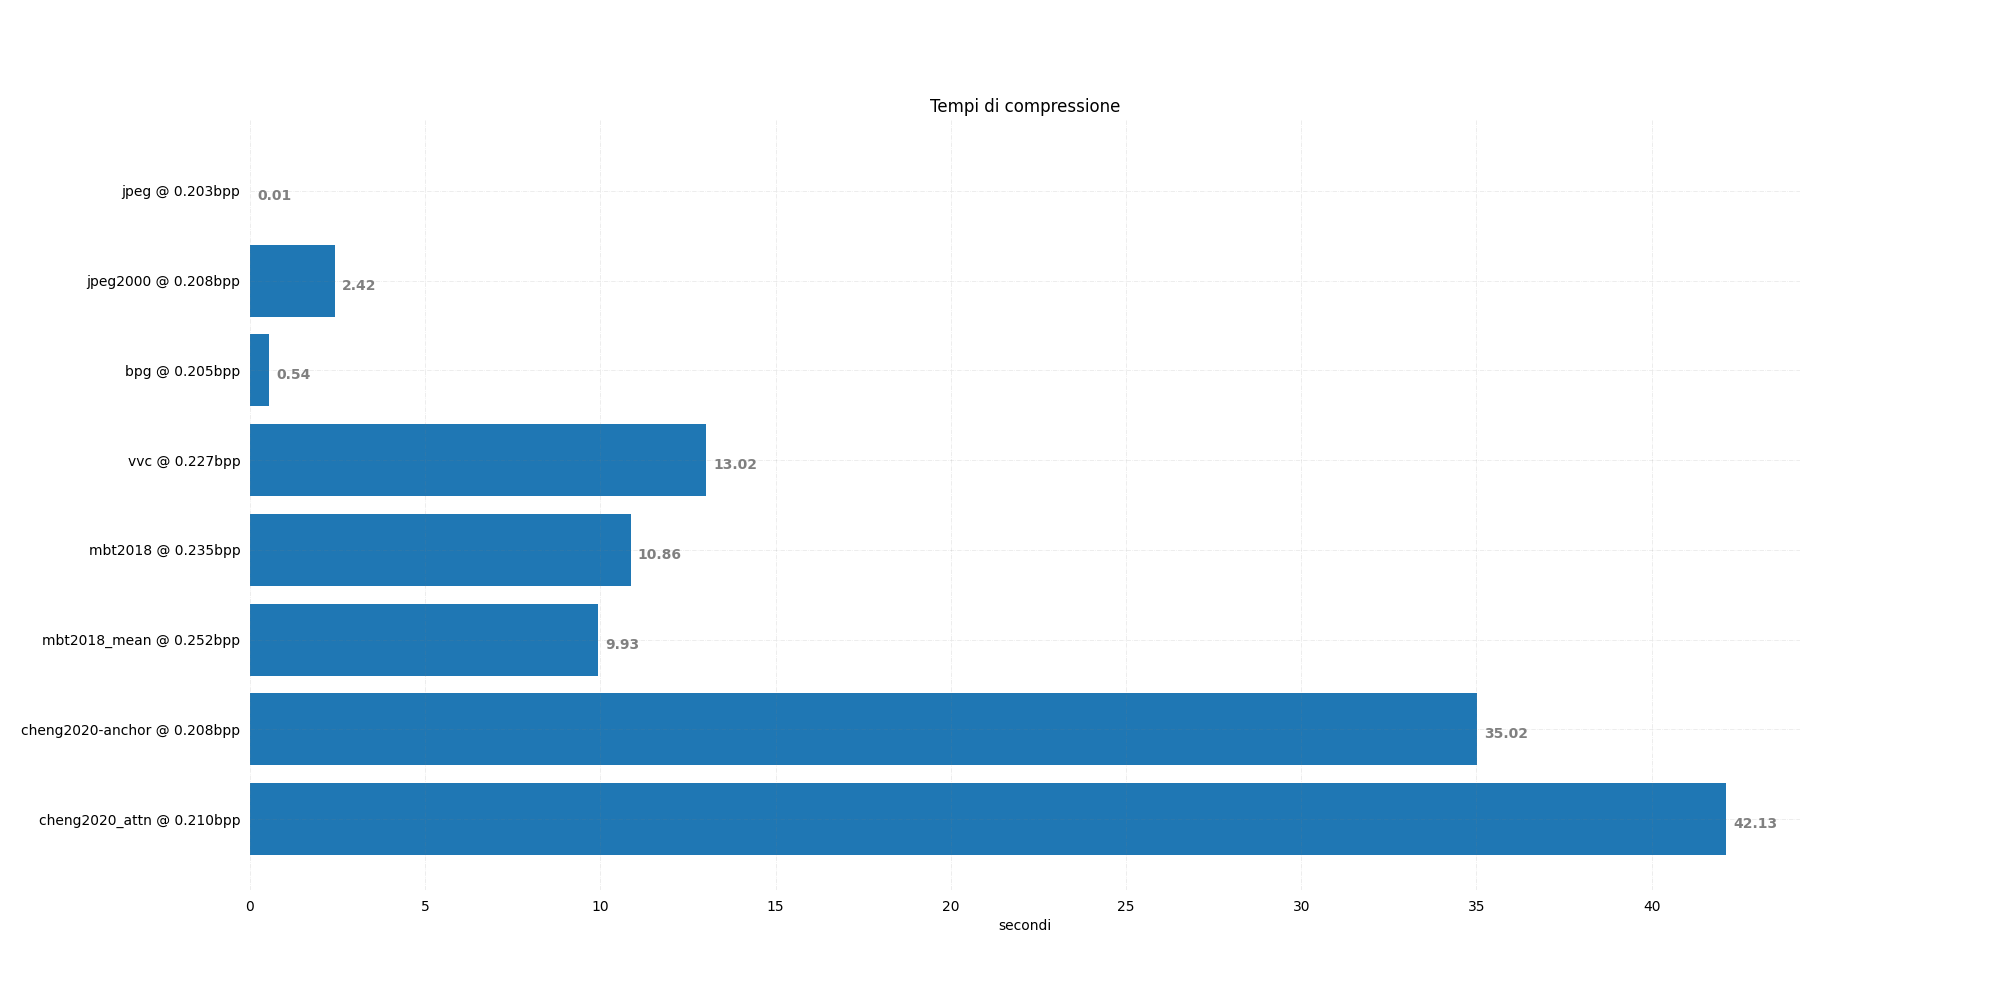
\includegraphics[width=1\textwidth]{Immagini/METRICS/times@0.21bpp.png}
    \caption{Tempi di compressione a 0.21 bpp}
    \label{fig:times21}
\end{figure}
\newpage
\begin{figure}[!h]
    \centering
    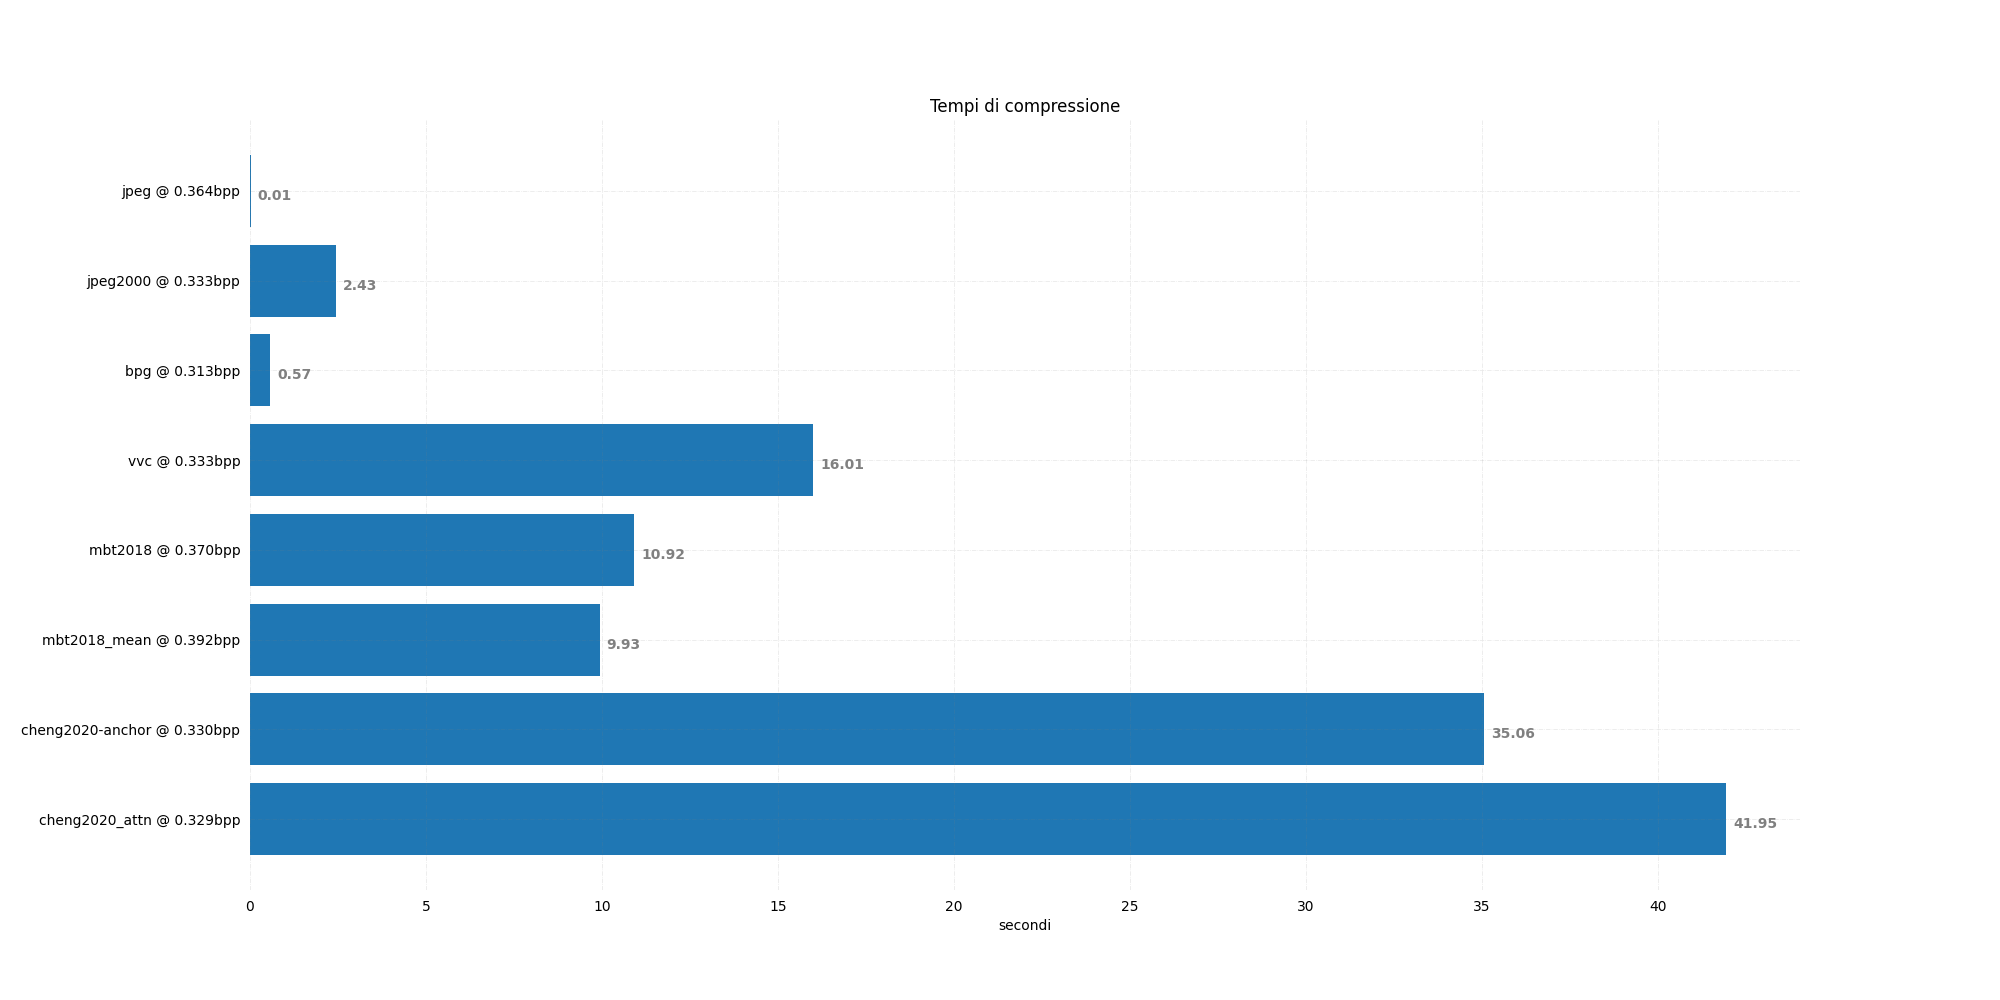
\includegraphics[width=1\textwidth]{Immagini/METRICS/times@0.34bpp.png}
    \caption{Tempi di compressione a 0.34 bpp}
    \label{fig:times34}
\end{figure}
\hspace{0.5cm}
\begin{figure}[!h]
    \centering
    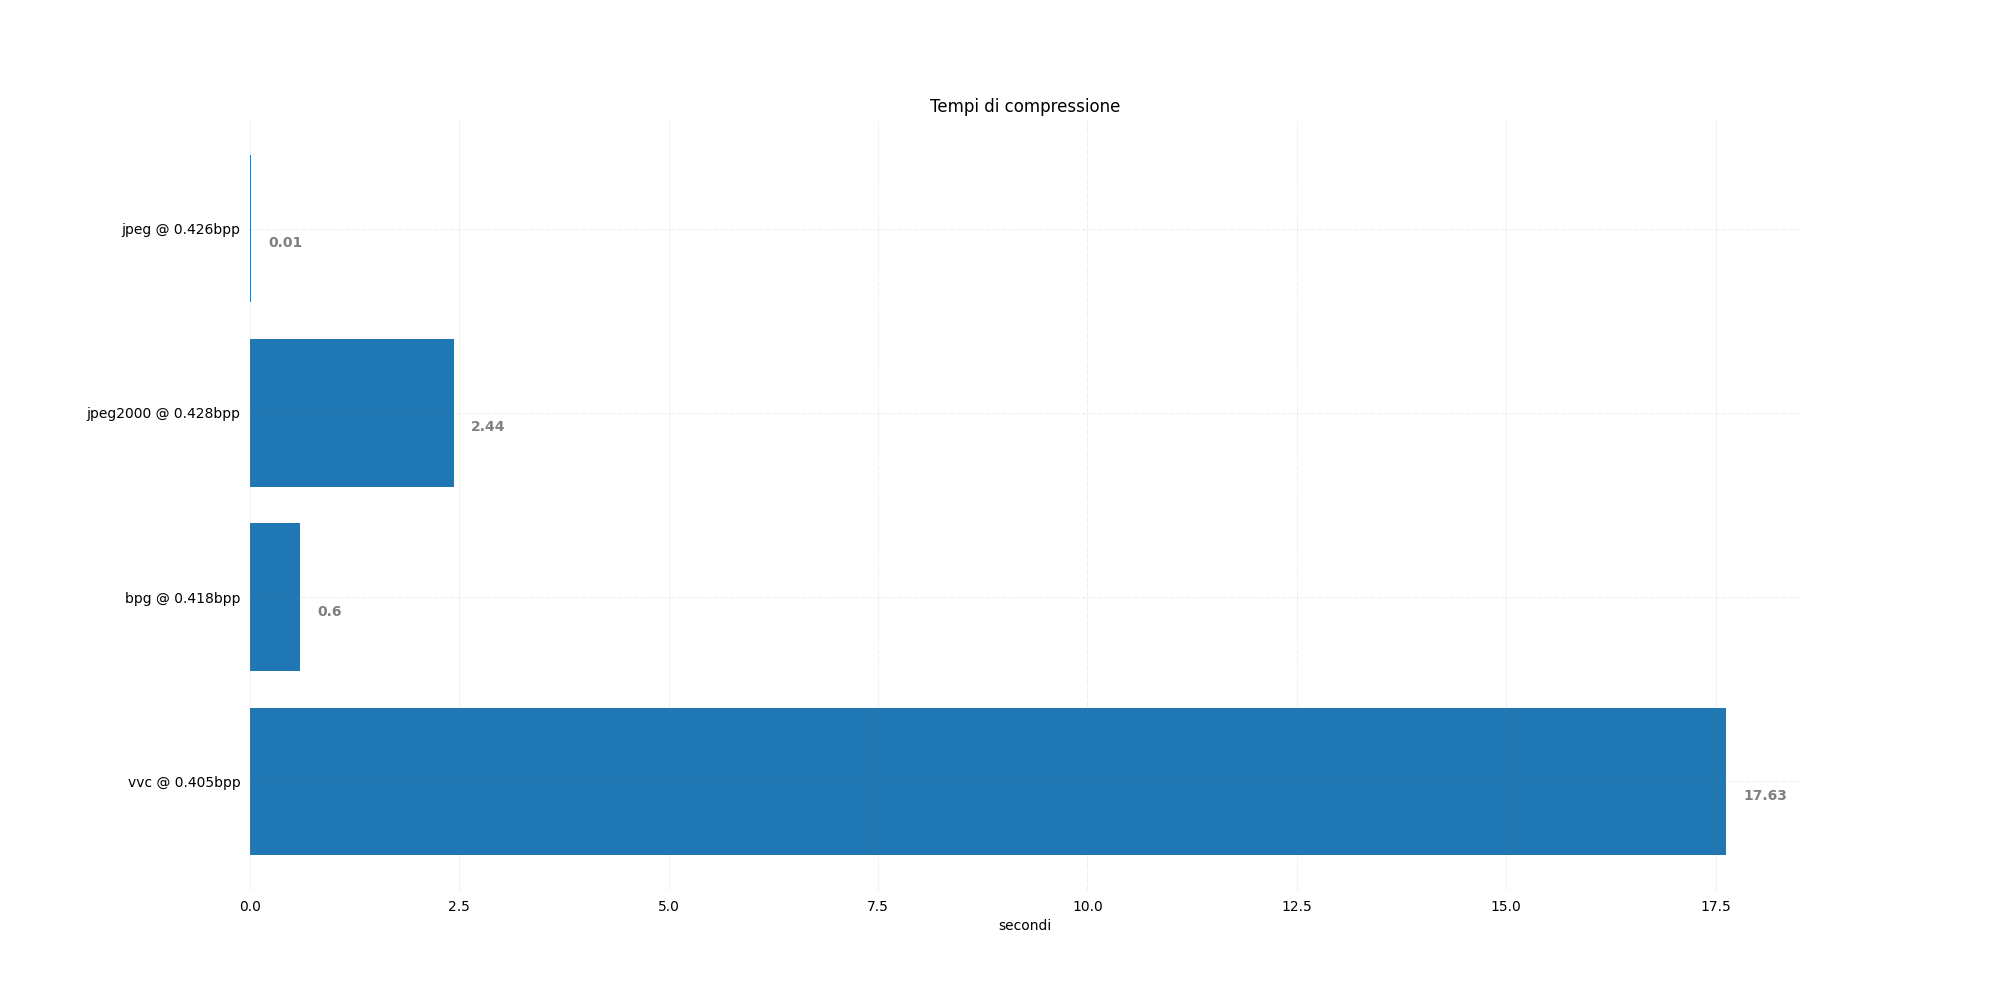
\includegraphics[width=1\textwidth]{Immagini/METRICS/times@0.41bpp.png}
    \caption{Tempi di compressione a 0.41 bpp}
    \label{fig:times41}
\end{figure}
\clearpage 
Come possiamo osservare nei grafici i tempi di compressione delle reti aumentano all’aumentare della qualità, i tempi di compressione dei metodi tradizionali invece non variano sensibilmente all’aumentare della qualità. Il codec VVC costituisce però un’eccezione a questo comportamento costante dei metodi tradizionali, in quanto possiamo vedere che il tempo aumenta all’aumentare della qualità. Questo comportamento si ha per la complessità di H.266, in quanto deve trovare il miglior metodo di compressione tra quelli a sua disposizione.\\
Passiamo ora a presentare le metriche di qualità dell’immagine, partiamo dal grafico del PSNR \ref{fig:PSNRGraph}, come possiamo vedere nel grafico, la migliore qualità di compressione si ha con il codec VVC, seguito poi da Cheng 2020, Ballé 2018, BPG, JPEG 2000 ed infine JPEG. H.266 si conferma quindi l’attuale stato dell’arte per la compressione di immagini osservando il grafico del PSNR, che ricordiamo essere una metrica oggettiva.\\
\begin{figure}[!h]
    \centering
    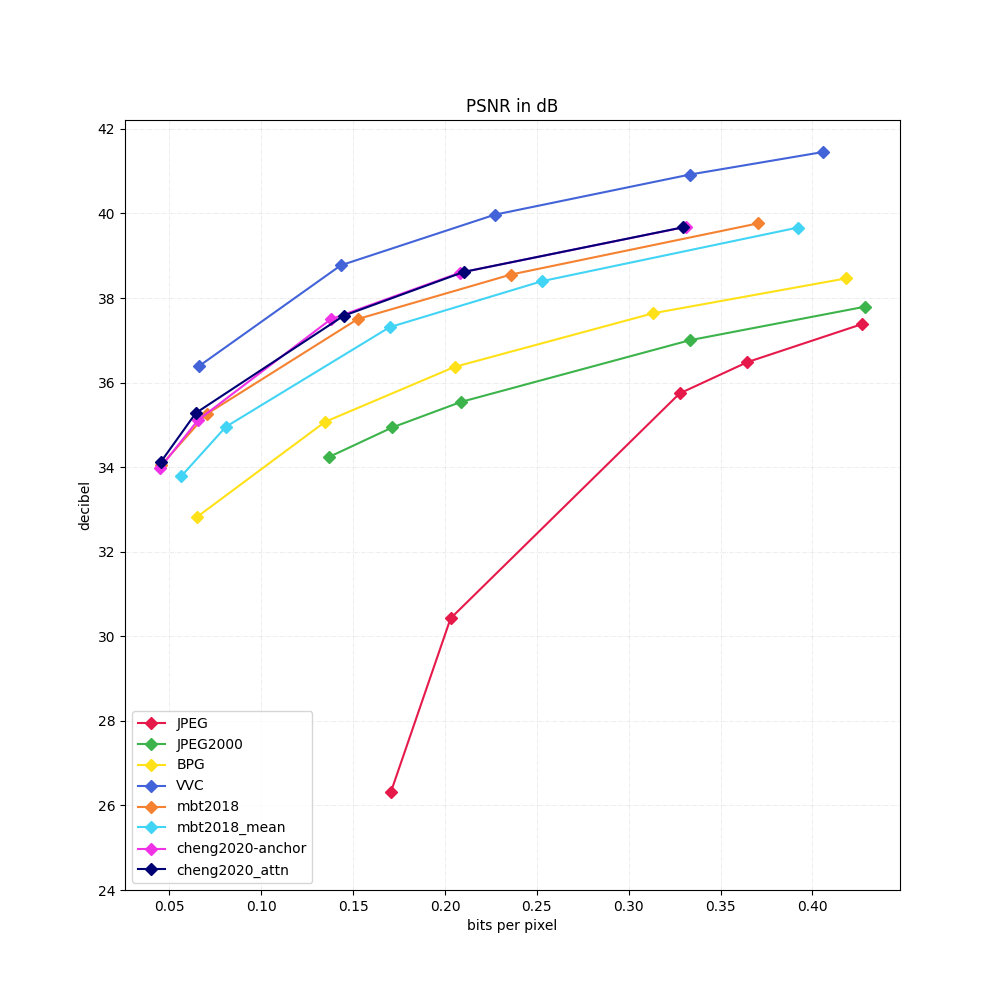
\includegraphics[width=0.9\textwidth]{Immagini/METRICS/PSNR.png}
    \caption{Grafico PSNR}
    \label{fig:PSNRGraph}
\end{figure}\\
Il prossimo grafico che andremo a commentare è il grafico dell’MS-SSIM \ref{fig:MSSSIMGraph}, in questo grafico possiamo osservare come JPEG, JPEG 2000 e BPG si confermino i metodi che forniscono le qualità di compressione peggiori. Diversamente da quanto osservato nel grafico del PSNR, secondo questo grafico il miglior metodo di compressione è Cheng2020, seguito da Balle2018 e come terzo abbiamo VVC.\\
Ricordiamo che l’MS-SSIM è invece una metrica che cerca di replicare la valutazione del sistema visivo umano.\\
\begin{figure}[!h]
    \centering
    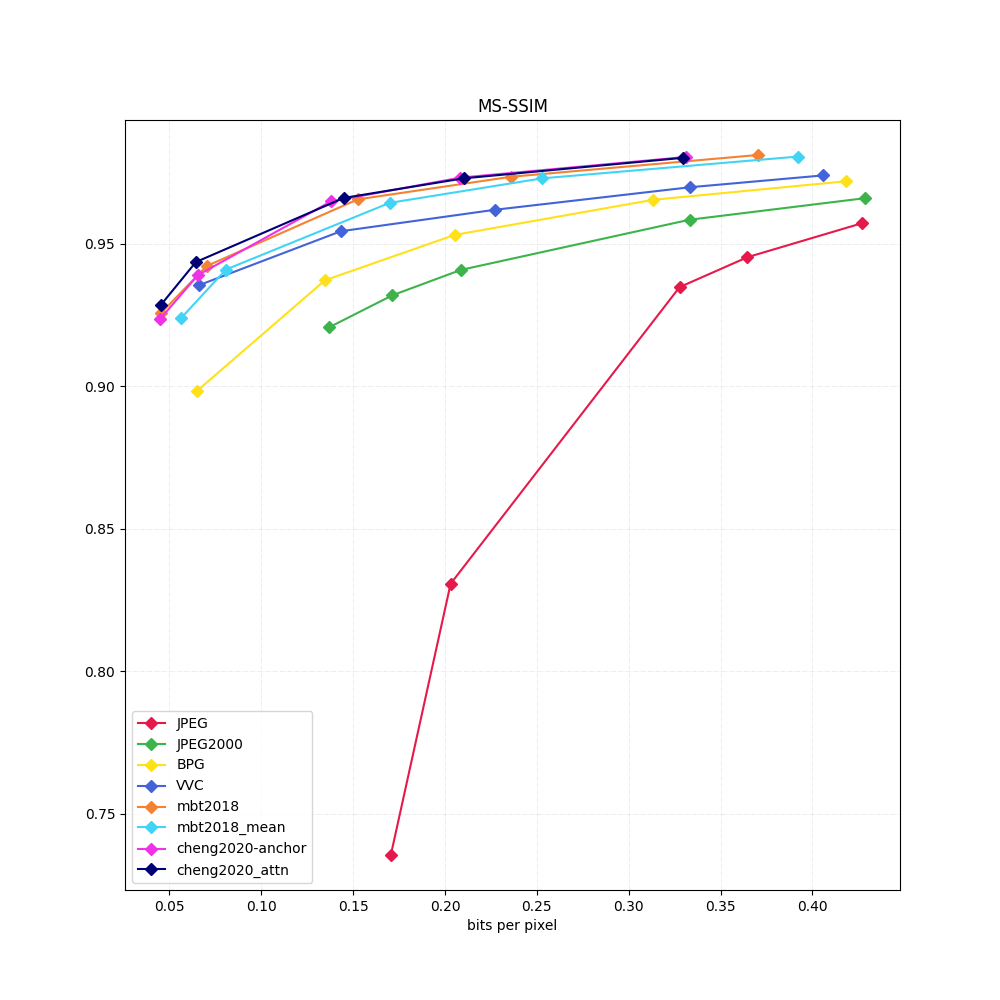
\includegraphics[width=0.9\textwidth]{Immagini/METRICS/MS-SSIM.png}
    \caption{Grafico MS-SSIM}
    \label{fig:MSSSIMGraph}
\end{figure}\\
L’ultima metrica è invece la più recente, andiamo ora a presentare i risultati presenti nel grafico della metrica LPIPS con AlexNet \ref{fig:LPIPSGraph}. Come possiamo vedere in questo grafico VVC si conferma il metodo migliore, seguito da Cheng2020, Ballé2018, BPG, JPEG 2000. Per quanto riguarda JPEG otteniamo un comportamento inaspettato in quanto i primi due punti sono in linea con le aspettative, il successivo invece è vicino a JPEG200 e gli ultimi due lo superano addirittura.\\
Questo comportamento ci ha sorpreso in quanto ci aspettavamo che la qualità percepita fosse vicina a quella di JPEG 2000 ma non che la superasse.\\
\begin{figure}[!h]
    \centering
    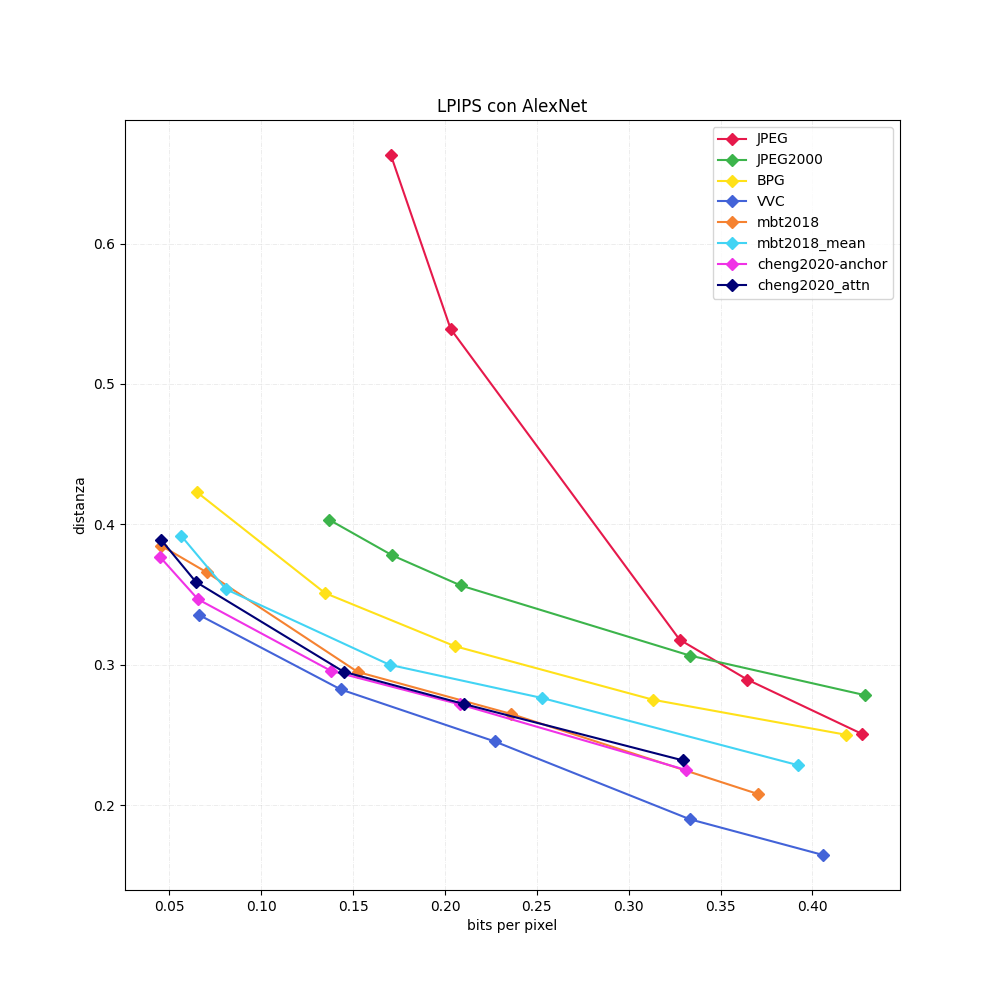
\includegraphics[width=0.9\textwidth]{Immagini/METRICS/LPIPS.png}
    \caption{Grafico LPIPS con AlexNet}
    \label{fig:LPIPSGraph}
\end{figure}\\
Dopo aver presentato e commentato questi grafici ci sentiamo di affermare che le reti da noi valutate svolgono un lavoro molto buono, che supera i metodi di compressione tradizionali più usati. Non riescono però ancora a superare il codec VVC che attualmente rimane lo stato dell’arte per la compressione di immagini.\\

    \chapter{Sviluppi futuri}

\section{Possibili ottimizzazioni}

\subsection{Spectral ADAM}

\section{Dispoitivi mobili}

\subsection{Small CAE}


    \chapter{Conclusioni}
Questo lavoro presenta l’attuale situazione per quanto riguarda la compressione di immagini con metodi tradizionali e che fanno uso di intelligenza artificiale. Nonostante i recenti avanzamenti nell’ambito di ricerca sulle intelligenze artificiali ci sentiamo di affermare che, alla luce degli esperimenti da noi eseguiti, le attuali reti, Ballé et al. \cite{minnen2018joint} e Cheng et al. \cite{cheng2020learned}, funzionano molto bene e potrebbero essere applicate nella vita di tutti i giorni, in quanto raggiungono prestazioni nettamente superiori rispetto ai metodi tradizionali più utilizzati, quali JPEG \cite{125072}, JPEG 2000 \cite{952804} e BPG \cite{BPGImageformat}, a discapito di una compressione più lenta eseguita su CPU, come possiamo vedere dai grafici \ref{fig:times07}, \ref{fig:times16}, \ref{fig:times21}, \ref{fig:times34}.\\
In casi specifici, dove è richiesta una qualità di compressione superiore invece, i metodi tradizionali e nello specifico VVC \cite{9503377}, rappresentano ancora l’unica alternativa sensata in quanto permettono di comprimere di più rispetto alle reti, garantendo una migliore qualità oggettiva e soggettiva, come possiamo osservare rispettivamente nei grafici \ref{fig:PSNRGraph} e \ref{fig:LPIPSGraph}.\\
L’ambito di ricerca della compressione con intelligenze artificiali rimane comunque molto promettente e con la crescente diponibilità di potenza di calcolo e di esempi di addestramento non potrà far altro che continuare a migliorare ulteriormente. Alcune migliorie potrebbero essere oggetto di future ricerche potrebbero essere l’uso di SpectralADAM \cite{balle2018efficient} per l’addestramento delle reti di compressione e l’attenzione nello sviluppo di reti riducibili, come slimCAE \cite{yang2021slimmable} sviluppata dal team di Yang et al. nel 2021, per permettere l’uso di questi metodi anche su dispositivi con ridotta potenza di calcolo.\\

    \cleardoublepage

    \printbibliography[heading=bibintoc]
\end{document}
